% reqno is needed to make the subnumcases have the case numbers on the right
% \documentclass[reqno]{amsart}
\documentclass[twoside,reqno]{report}
% \usepackage[top=1in, bottom=1in, left=1.5in, right=1in, includehead]{geometry}
% \documentclass{article}
% \documentclass[runningheads]{llncs}
% \documentclass[preview]{standalone}
\usepackage{twoopt}
\usepackage{tabularx,booktabs}
% \usepackage{array}
\renewcommand\tabularxcolumn[1]{m{#1}}
\newcommand{\LukaTable}[2][2]{\LukaTableDriver[.36][.22]{8}{#1}{#2}}
\newcommandtwoopt{\LukaTableDriver}[5][1][1]{
  \begin{tikzpicture}[x=#1cm, y=#2cm, step=1]
      \tikzmath{
        \xValue = 0;
        \yValue = 0;
        {
          \draw[black,thin] (0,0) grid (#3,#4);
          \filldraw[fill=none, draw=none] (#3, #4) ellipse (0.05cm and 0.05cm);  % for consistent bounding box
        };
        for \yDelta in {#5}{
          %\labelUp = int(\yDelta+1);
          %\labelDn = int(\yDelta);
          {
            \filldraw[fill=black, draw=black] (\xValue, \yValue) ellipse (0.05cm and 0.05cm);
            %\node[] at (\xValue + 0.5, -1) {\labelDn};
            %\node[] at (\xValue + 0.5, #3) {\labelUp};
          };
          \xNext = \xValue + 1;
          \yNext = \yValue + \yDelta - 1; % Here is the -1
          {
            \draw[black,very thick] (\xValue, \yValue) -- (\xNext, \yNext);
          };
          \xValue = \xNext;
          \yValue = \yNext;
        };
      }
      {
        \filldraw[fill=black, draw=black] (\xValue, \yValue) circle (0.05cm);
      };
  \end{tikzpicture}
}

% \newcommand*{\thead}[1]{%
% \multicolumn{1}{c}{\bfseries\begin{tabular}{@{}c@{}}#1\end{tabular}}}
\newcolumntype{C}{>{\centering\arraybackslash}X}

\usepackage{mathtools}
\usepackage[english]{babel}
% \usepackage{tabularx}
\usepackage{tikz}
\usepackage{xcolor}

% stuff for making verbatim work better
\usepackage{fancyvrb}
\usepackage{cprotect}

% TODO: maybe get nicer colors
\definecolor{p1col1}{rgb}{1.0, 0, 0}
% \definecolor{p1col1}{RGB}{80, 0, 130}
\definecolor{p1col2}{rgb}{0, 1.0, 0}
% \definecolor{p1col2}{RGB}{255, 190, 10}
\definecolor{p1col3}{rgb}{0, 0, 1.0}
% \definecolor{p1col3}{RGB}{255, 190, 10}
\definecolor{p1col4}{rgb}{0, 0, 0}
\definecolor{lightpurple}{RGB}{203, 195, 227}
% \definecolor{midpurple}{RGB}{243, 225, 247}
\definecolor{lightblue}{RGB}{173, 216, 230}
\definecolor{lightyellow}{RGB}{255, 255, 158}

% \definecolor{p1col4}{RGB}{40, 0, 80}

\usepackage{graphicx}

\usepackage{verbatim}
\usepackage{amsfonts}
\usepackage{amssymb}
\usepackage{amsmath}
\usepackage{amsthm}

\usepackage{xcolor}
\usepackage{colortbl}

\usepackage{algorithm}
\usepackage[noend]{algpseudocode}


\usepackage{twoopt}
\usepackage{tikz}
\usepackage{tikz-qtree}
\usetikzlibrary{math}

% \usepackage{caption}
\usepackage[justification=centering]{caption}
\usepackage{subcaption}

\usepackage[title]{appendix}

\usepackage{verbatim}

\newcommand{\emptystring}{\varepsilon}

\usepackage{cases}





%
% Algorithm environment commands
%
% https://tex.stackexchange.com/questions/74880/algorithmicx-package-comments-on-a-single-line
\algnewcommand{\LineComment}[1]{\State \(\triangleright\) #1}

% https://tex.stackexchange.com/questions/184154/algorithmic-put-if-and-endif-into-same-line
\algnewcommand{\OneLineIf}[2]{\State\algorithmicif\ #1\ \algorithmicthen\ #2}

% https://tex.stackexchange.com/questions/234690/and-in-algorithm
\algnewcommand{\algorithmicand}{\textbf{ and }}
\algnewcommand{\algorithmicor}{\textbf{ or }}
\algnewcommand{\algorithmicnot}{\textbf{ not }}
\algnewcommand{\OR}{\algorithmicor}
\algnewcommand{\AND}{\algorithmicand}
\algnewcommand{\NOT}{\algorithmicnot}

\newcommand{\visit}[1]{\texttt{visit}(#1)}
% \newcommand{\visit}[1]{\texttt{visit}(#1)}

% \newcommand{\pshift}[2][]{$\mathsf{preshift}_{#1}(#2)$}
\newcommand{\transpose}[3]{\mathsf{transpose(} #1, #2, #3 \mathsf{)}}
\newcommand{\preshift}[2]{\mathsf{preshift(} #1, #2 \mathsf{)}}

% \newcommand{\leftshift}[2]{\mathsf{leftshift(} #1, #2 \mathsf{)}}
\newcommand{\treeshift}[3]{\mathsf{shiftfirst(} #1, #2, #3 \mathsf{)}}
\newcommand{\popchild}[1]{\mathsf{popchild(} #1 \mathsf{)}}
\newcommand{\pushchild}[2]{\mathsf{pushchild(} #1, #2 \mathsf{)}}
% \newcommand{\poppush}[2]{\mathsf{poppush(} #1, #2 \mathsf{)}}
\newcommand{\poppush}[3][]{\mathsf{poppush}_{#1}(#2,#3)}
% \newcommand{\poppushopt}[2][]{\mathsf{poppush}_{#1}( #2, #3 \mathsf{)}}


% https://tex.stackexchange.com/questions/228474/bold-horizontally-and-vertically-aligned-multiline-table-headers
\newcommand*{\thead}[1]{%
\multicolumn{1}{c}{\bfseries\begin{tabular}{@{}c@{}}#1\end{tabular}}}


    % TODO: might not actually need these
\newcommand{\leftshift}[3][]{\mathsf{left}_{#1}(#2,#3)}

\newcommand{\nextPrefix}[1]{\mathsf{next}{(#1)}}
\newcommand{\nextTree}[1]{\mathsf{nextree}{(#1)}}
\newcommand{\coolCat}[1]{\overrightarrow{\mathsf{coolCat}}{(#1)}}
\newcommand{\otree}[1]{\mathsf{OTree}{(#1)}}
\newcommand{\dyck}[1]{\mathsf{Dyck}{(#1)}}
\newcommand{\dyckindex}[1]{\mathsf{DyckIndex}{(#1)}}

\newcommand{\otreenode}[1]{\mathsf{OTreeNode}{(#1)}}
\newcommand{\leftdown}[1]{\mathsf{leftpath}{(#1)}}
\newcommand{\depth}[1]{\mathsf{Depth}{(#1)}}
% \newcommand{\ithone}[2]{\mathsf{i^{\underline{th}}one}_{#1}{(#2)}}
\newcommand{\oneindex}[2]{\mathsf{oneindex}({#1}, #2)}
\newcommand{\zeroesbetween}[3]{\mathsf{zeroesbetween({#1}, #2, #3)}}
\newcommand{\thh}{^{\underline{th}}}
% \newcommand{\path}[2]{\mathsf{path}({#1}, #2)}
\newcommand{\path}[3]{\mathsf{path({#1}, #2, #3)}}



\usepackage{tabularx,booktabs}
\usepackage[letterpaper,top=2cm,bottom=2cm,left=3cm,right=3cm,marginparwidth=1.75cm]{geometry}

\usepackage{amsmath}
\usepackage{graphicx}
\usepackage[colorlinks=true, allcolors=blue]{hyperref}

% THEOREM STUFF
\newtheorem{theorem}{Theorem}[section]
\newtheorem{lemma}[theorem]{Lemma}
% \newtheorem{theorem}{Theorem}[section]
\newtheorem{remark}{Remark}
% \newtheorem{lemma}[theorem]{Lemma}

\title{Cooler than Cool: \\ Cool-Lex Order for Generating New Combinatorial Objects}
\author{Paul Lapey}


\begin{document}
\maketitle
\tableofcontents
% Two primary contributions, each with subcontributions
% each new result: one section on gray code, one section on implementation


% figure balanced parentheses binary trees
% add figures/exhaustive lists
\section{Combinatorial Generation: Looking at All the Possibilities}

Combinatorial generation is defined as the exhaustive listing of combinatorial objects of various types.  Frank Ruskey duly notes in his book \emph{Combinatorial Generation} that the phrase ``Let's look at all the possibilities" sums up the outlook of his book and the field as a whole \cite{ruskey2003combinatorial}. Examining all possibilities fitting certain criteria is frequently necessary in fields ranging from mathematics to chemistry to operations research. Combinatorial generation as an area of study seeks to find an underlying combinatorial structure to these possibilities and utilize it to obtain an algorithm to efficiently enumerate an appropriate representation of them \cite{ruskey2003combinatorial}. 

Combinatorial generation has many parallels to sorting.  It is a fundamental computational task that will continue to be a necessary part of solving difficult problems for the foreseeable future.  Additionaly, different sorting algorithms are often better suited for for different types of data.  For example, bubble sort is generally slower than merge sort, but can be faster when the initial data is already close to being in sorted order. Similarly, different combinatorial generation algorithms may be better suited for different types of tasks.  This makes combinatorial generation an important area of study for making many common tasks more efficient.  

Unlike sorting, however, combinatorial generation is not widely taught and is rarely discussed in core textbooks. The foundational textbook series The Art of Computer proramming was initially released in 1968; combinatorial generation was not discussed until volume 4A, released in 2011 \cite{knuth2015art}.  Another notable combinatorial generation textbook is  Kreher and Stinson's \emph{Combinatorial Algorithms: Generation, Enumeration, and Search} \cite{kreher2020combinatorial}. Outside of these, however, discussion of combinatorial generation in textbooks is rare.

\section{Lexicographic Orders}
    Lexicographic order is the simplest and most intuitive way of enumerating combinatorial objects.  As its name suggests\footnote{\emph{Lexicography} is a word for the practice of compiling dictionaries.  It draws its roots from the Greek \textlambda\textepsilon\textxi\textiota\textkappa\textomikron$\varsigma$ \ (lexikos), meaning ``of words," and \textgamma\textrho\textalpha\textphi\texteta \  (graphe), meaning drawing or writing.  Lexicography, therefore, can be thought of as writing about words.  Interestingly, \textlambda\textepsilon\textxi\textiota\textkappa\textomikron$\varsigma$ and the English words \emph{lecture}, \emph{legend}, \emph{legible}, and \emph{legume}, all stem from the same Proto-Indo-European word meaning to collect.  Reconstructing a common thread among these etymologically related words is left as an exercise to the reader.}, it is the order typically used to order words in a dictionary.  Any language of strings formed from a set of symbols with a total ordering has a lexicographic ordering.  In particular, a lexicographic ordering is a total order of strings formed from symbols with a total ordering.  An additional benefit of lexicographic ordering is that listing a set of combinatorial objects in lexicographic order is always possible. Any combinatorial object handled by computers must be encoded in binary somehow; therefore any combinatorial object can be enumerated in lexicographic order via the lexicographic order of its binary representations. 

% TODO: different ways to implement lex (i.e., scan for location of change, or keep track and predict) ? 

In addition to traditional lexicographic order, there are several closely related variations of it. Co-lexicographic order generates objects as if they were being generated via a lexicographic ordering of strings read in reverse.  Where lexicographic order increments the rightmost bit and carries to the left, co-lexicographic order increments the leftmost bit and carries to the right. Reverse lexicographic order generates objects in the reverse order of lexicographic order: it order objects from lexicographically largest to lexicographically smallest. Co-lexicographical order can also be reversed in this way to generate reverse co-lexicographic order. Figure \ref{fig:bintable} demonstrates lexicographic, co-lexicographic, and reverse lexicographic order for binary strings with $n$ bits.  Although all four lexicographic orderings are similar for binary strings, they are often very different from each other for for enumerating other sets of objects.

Continuing with the comparison of combinatorial generation to sorting, lexicographic and co-lexicographic orders are much like insertion and selection sort.  They are fairly intuitive, easy to implement, and sometimes ``good enough."  However, they are rarely optimal: more thoughtful orderings will frequently have significant performance advantages over lexicographic orderings. In particular, lexicographic orderings often require worst-case $O(n)$ time per generated object, whereas \emph{loopless} generation algorithms that use worst-case constant time per generated object are often achievable. The term loopless refers to the fact that, typically, a worst-case $O(1)$ algorithm can be implemented without any inner loops.

 \subsection{Lexicographic Sublists}
 An interesting observation is that lexicographic orderings for any fixed length binary language can be obtained by filtering the lexicographic ordering of all binary strings to obtain a sub-list. Specificaly, if a language $\mathcal{L}$ is a subset of $n$-bit binary strings, generate all $n$-bit binary strings and filter the list to contain only strings in $\mathcal{L}$.  The resulting list will be a lexicoraphic ordering of the strings in $\mathcal{L}$.  The same property holds for co-lexicographic order, reverse lexicographic order, and reverse co-lexicographic order.  Figure \ref{fig:bintable} illustrates generating $4$-bit binary strings and filtering that list to obtain a sublist of binary strings with $2$ ones and $2$ zeroes.  It does this for lexicographic orderings, the binary reflected Gray code to be discussed in \ref{sec:BRGC}, and cool lex order, discussed in \ref{sec:coolIntro}.


 \begin{figure}[]

     \begin{subfigure}[]{\textwidth}
         \begin{center}
         \caption{The $2^4$ $4$-bit binary strings generated lexicographic, co-lexicographic, reverse lexicographic, reverse co-lexicographic, binary reflected Gray code, and cool-lex order.}
             \begin{tabular}{ |c|c|c|c|c||c||c| } 
                 \hline
                 n &  lex  & colex & revlex & revcolex & Gray & cool\\  
                 \hline
                 0 & 0000 & 0000 & 1111 & 1111 & 0000   & 0000  \\
                 1 & 0001 & 1000 & 1110 & 0111 & 0001   & 1000  \\
                 2 & 0010 & 0100 & 1101 & 1011 & 0011   & 1100  \\
                 3 & 0011 & 1100 & 1100 & 0011 & 0010   & 1110  \\
                 4 & 0100 & 0010 & 1011 & 1101 & 0110   & 1111  \\
                 5 & 0101 & 1010 & 1010 & 0101 & 0111   & 0111  \\
                 6 & 0110 & 0110 & 1001 & 1001 & 0101   & 1011  \\
                 7 & 0111 & 1110 & 1000 & 0001 & 0100   & 1101  \\
                 8 & 1000 & 0001 & 0111 & 1110 & 1100   & 0110  \\
                 9 & 1001 & 1001 & 0110 & 0110 & 1101   & 1010  \\
                 10 & 1010 & 0101 & 0101 & 1010 & 1111  & 0101  \\
                 11 & 1011 & 1101 & 0100 & 0010 & 1110  & 0011  \\
                 12 & 1100 & 0011 & 0011 & 1100 & 1010  & 1001  \\
                 13 & 1101 & 1011 & 0010 & 0100 & 1011  & 0100  \\
                 14 & 1110 & 0111 & 0001 & 1000 & 1001  & 0010  \\
                 15 & 1111 & 1111 & 0000 & 0000 & 1000  & 0001  \\
                 \hline
             \end{tabular}
         \end{center}
         \label{fig:bin4}
     \end{subfigure}
     \begin{subfigure}[]{\textwidth}
         \begin{center}
         \caption{4-bit binary strings filtered to only contain strings with 2 ones and 2 zeroes}
             \begin{tabular}{ |c|c|c|c|c||c||c| } 
                 \hline
                 n &  lex  & colex & revlex & revcolex & Gray & cool\\
                 \hline
                 0 &      &      &      &      &       &      \\
                 1 &      &      &      &      &       &      \\
                 2 &      &      &      &      & 0011  & 1100 \\
                 3 & 0011 & 1100 & 1100 & 0011 &       &      \\
                 4 &      &      &      &      & 0110  &      \\
                 5 & 0101 & 1010 & 1010 & 0101 &       &      \\
                 6 & 0110 & 0110 & 1001 & 1001 & 0101  &      \\
                 7 &      &      &      &      &       &      \\
                 8 &      &      &      &      & 1100  & 0110 \\
                 9 & 1001 & 1001 & 0110 & 0110 &       & 1010 \\
                 10 & 1010 & 0101 & 0101 & 1010 &      & 0101 \\
                 11 &      &      &      &      &      & 0011 \\
                 12 & 1100 & 0011 & 0011 & 1100 & 1010 & 1001 \\
                 13 &      &      &      &      &      &      \\
                 14 &      &      &      &      & 1001 &      \\
                 15 &      &      &      &      &      &      \\
                 \hline
             \end{tabular}
         \end{center}
         \label{fig:bin4to2c2}
     \end{subfigure}
     \begin{subfigure}[]{\textwidth}
         \caption{Condensed version of the orders for binary strings with 2 ones and 2 zeroes obtained above}
         \begin{center}
             \begin{tabular}{ |c|c|c|c||c||c| } 
                 \hline
                 lex  & colex & revlex & revcolex & Gray & cool\\
                 \hline
                 0011 & 1100 & 1100 & 0011 & 0011 & 1100 \\
                 0101 & 1010 & 1010 & 0101 & 0110 & 0110 \\
                 0110 & 0110 & 1001 & 1001 & 0101 & 1010 \\
                 1001 & 1001 & 0110 & 0110 & 1100 & 0101 \\
                 1010 & 0101 & 0101 & 1010 & 1010 & 0011 \\
                 1100 & 0011 & 0011 & 1100 & 1001 & 1001 \\
                 \hline
             \end{tabular}
         \end{center}
         \label{fig:2c2}
     \end{subfigure}
     \begin{center}

     \end{center}
     \caption{The $2^4$ $4$-bit binary strings generated lexicographic, co-lexicographic, reverse lexicographic, reverse co-lexicographic, binary reflected Gray code, and cool-lex order.}
     \label{fig:bintable}
 \end{figure}


\section{Binary Reflected Gray Code} \label{sec:BRGC}

A quintessential result of combinatorial generation in practice is Frank Gray's reflected binary code, or Gray code. The binary reflected Gray code gives a ``reflected" ordering of binary strings such that each successive string in the ordering differs from the previous string by exactly one bit. This contrasts from a lexicographic ordering of binary strings, in which a n-digit binary string can differ by up to n digits from its predecessor and will differ by approximately two (more precisely $\sum_{i=0}^n\frac{1}{2}^i$, which is 1.9375 for 4 bit values and 1.996 for 8 bit values) bits on average\footnote{Consecutive pairs of binary digits in lexicographic order will differ in the bit at position i with probability $\frac{1}{2}^i$.  Therefore, the average number of differing bits between two binary strings of length n is $\sum_{i=0}^n\frac{1}{2}^i$, which converges to 2 as n grows large.}. The binary reflected Gray code, therefore, provides an ordering that requires half as many bit switches on average as the more intuitive lexicographic order. 

The iterative successor rule for the binary reflected Gray code has 2 cases and is as follows:


Let $\alpha$ be a binary string and let $f$ be the first bit of $\alpha$ that is equal to 1.

\begin{equation} \label{eq:BRGC-rule}
    \text{gray}(\alpha) = \begin{cases} 
        \complementbit{1} & \text{if the parity of $\alpha$ is even}\\
        \complementbit{f+1} & otherwise\\
\end{cases}
\end{equation}

Binary reflected Gray codes are especially useful in electromechanical switches to reduce physical error and prevent spurious output associated with asynchronous bit switches.  In particular, changing multiple bits per iteration can result in ``in-between" states where some but not all of the bit changes necessary for a switch have been executed.  One can think of this like an odometer on a car: When changing from $99999$ to $100000$ miles, the odometer might briefly read $000000$, or $19999$, or $10009$, or any number of other ``in-between" states. 

This issue can occur in cases as simple as incrementing $3$ to $4$.  In lexicographic order, the string must change from $011$ to $100$; in Gray code order it changes from $010$ to $110$.  The lexicographic change requires three bit changes; the Gray code order requires only one.  When using physical switches, three bit changes are unlikely to change in exact synchrony.  This creates the possibility of reading $101$, $110$, $111$, or \emph{any other 3-bit binary number} if the switches are read mid-change, depending on the order of the bit changes.  When using the binary reflected Gray code, the only states are $3=010$, the previous value, and $4=110$, the correct next value. One could easily imagine a test, such as checking if a number is less than $5$, that could evaluate incorrectly due to reading during the change between $3=011$ and $4=100$ in lexicographic order.  This type of error is eliminated by using a Gray code ordering that changes only one bit per iteration.


Frank Gray's binary reflected code was influential enough that the term \emph{Gray code} is often used as a general term for any minimal change ordering of combinatorial objects.  If lexicographic orderings with worst-case $O(n)$ time per generated object are like $O(n^2)$ sorting algorithms, Gray codes are like more efficient sorting algorithms such as merge sort, quick sort\footnote{Quicksort is actually worst-case $O(n^2)$, but has better average performance than simple $O(n \log(n))$ sorting algorithms like mergesort or heapsort.  This is due to space efficiency and cache performance, among other things.  Other sorting algorithms like introsort, pdqsort, and Timsort use hybrid approaches to obtain quicksort-like (or better) average performance while maintaining $O(n \log(n))$ worst-case runtime.}, or radix sort.  Gray codes perform iterations by modifying a single object in place, not generating a new object from scratch.  This is almost a hard requirement for achieving better than $O(n)$ time per object, as generating an object of size $n$ from scratch is always at least $O(n)$.

% \subsubsection{Sublists: Reflecting and Filtering}
% Inspired similar minimal change orders in two distinct ways: taking sublists, and generalizin reversing approach.

\subsection{Gray Code Sublists}
In particular, Gray codes for many binary languages can be obtained by listing all binary strings in Gray code order, filtering the list to contain only strings in the language, and seeing if the resulting ordering is a Gray code.  Sawada, Williams, and Wong demonstrated this process in practice for a broad set of binary ``flip-swap languages" including necklaces, Lyndon words, and feasible 0-1 knapsack problem solutions, among others \cite{sawada2021inside}.  They found that orderings obtained for binary ``flip-swap'' languages by filtering the binary reflected Gray code all have the property that successive strings differ from each other by at most 2 bits, allowing for simple and efficient implementations of these orderings.


\begin{figure}
    \centering

\includegraphics[width=4in]{BLX6-cropped.pdf} 


\includegraphics[width=4in]{BRGC6-cropped.pdf} 


\includegraphics[width=4in]{BCLX6-cropped.pdf} 

    \caption{A visual representation of Lexicographic (top), binary reflected Gray code (middle), and cool-lex (bottom) enumerations of 6-bit binary strings. Individual strings are read vertically with the most significant bit at the top; white is 1.
    }
    \label{binary}
\end{figure}

\section{Cool-Lex Order} \label{sec:coolIntro}

Cool-lex order can most easily be introduced using marbles on a ramp. Suppose one has $n$ marbles on a ramp, with each marble colored black or white.  

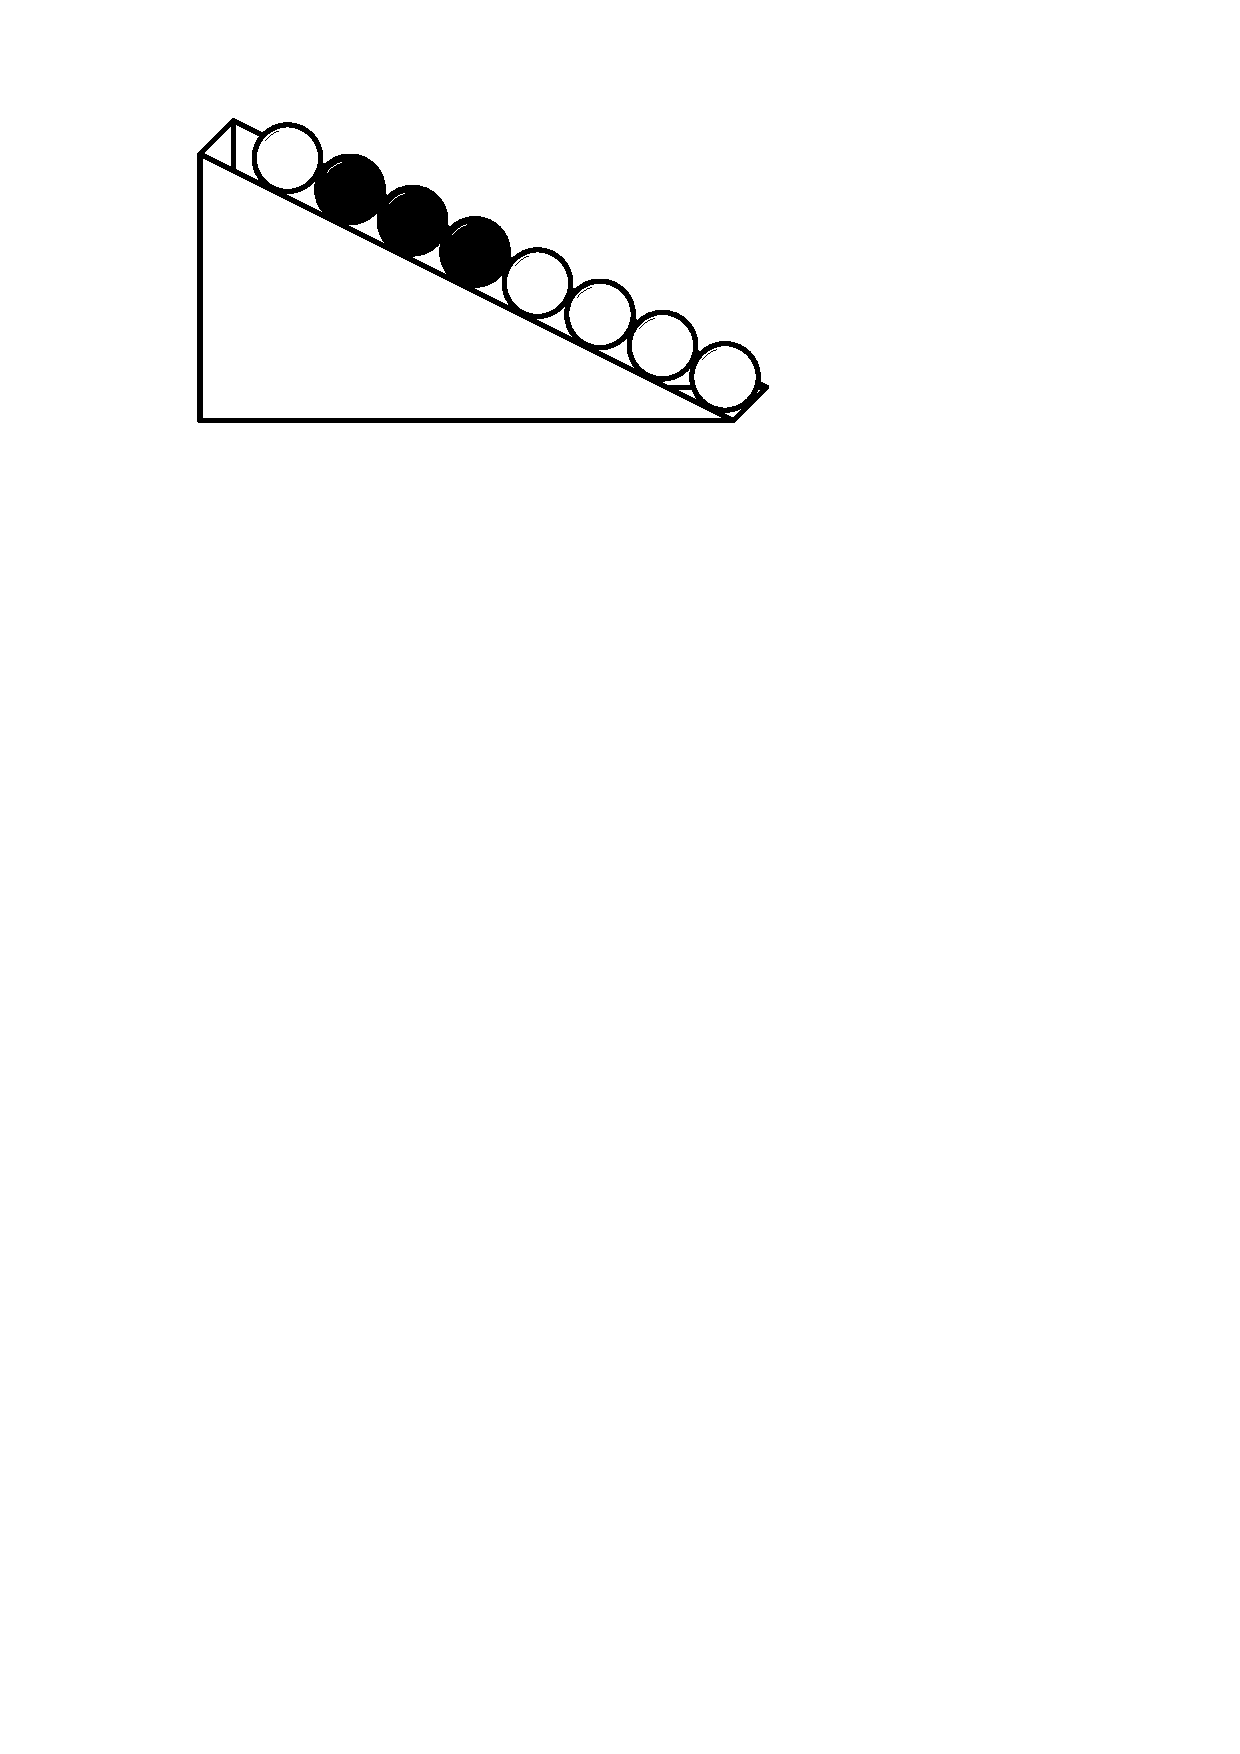
\includegraphics[width=.3\textwidth]{figures/marbles_first.pdf} 


Let $x$ be the first black marble that follows a white marble. Consider picking up and moving marble $x+1$ to the top of the ramp. This yields a new configuration.

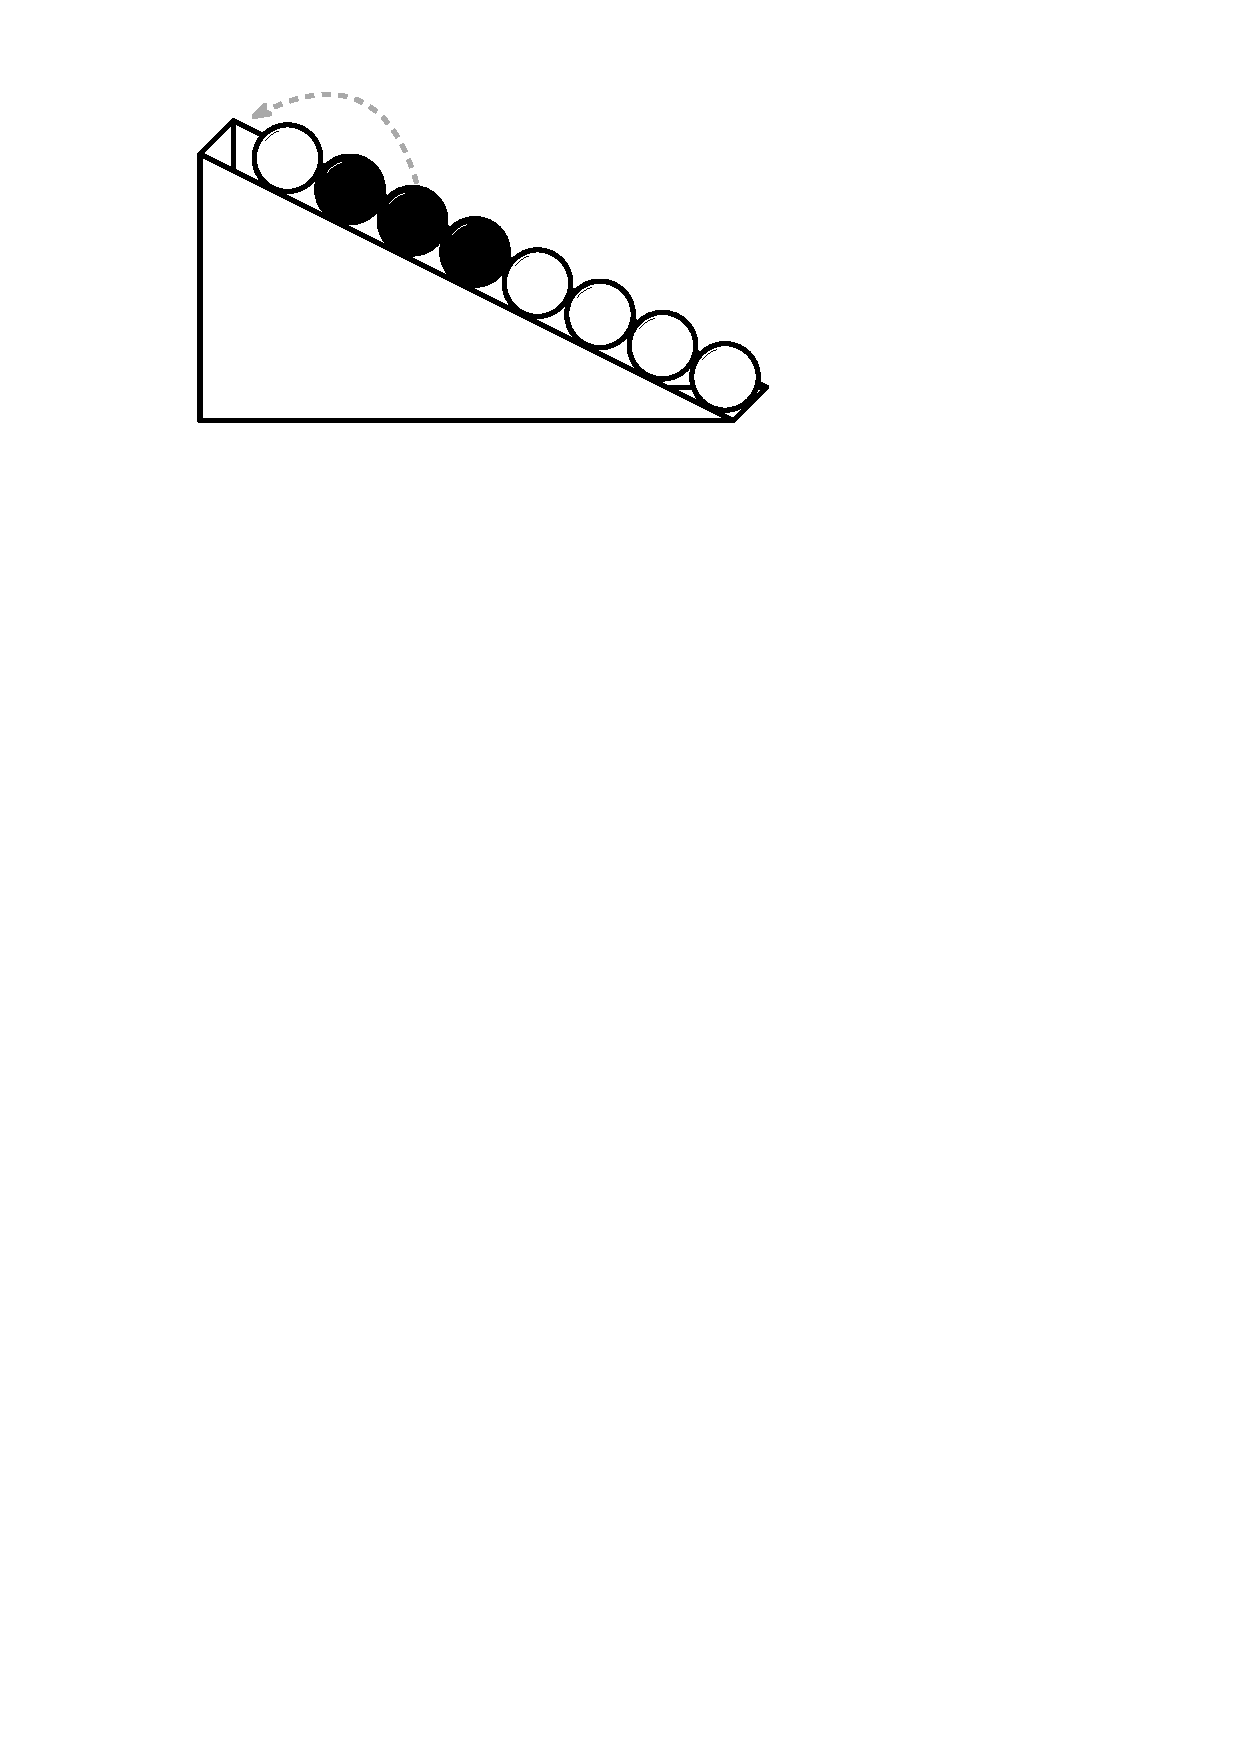
\includegraphics[width=.3\textwidth]{figures/marbles_first_arrow.pdf} $\implies$
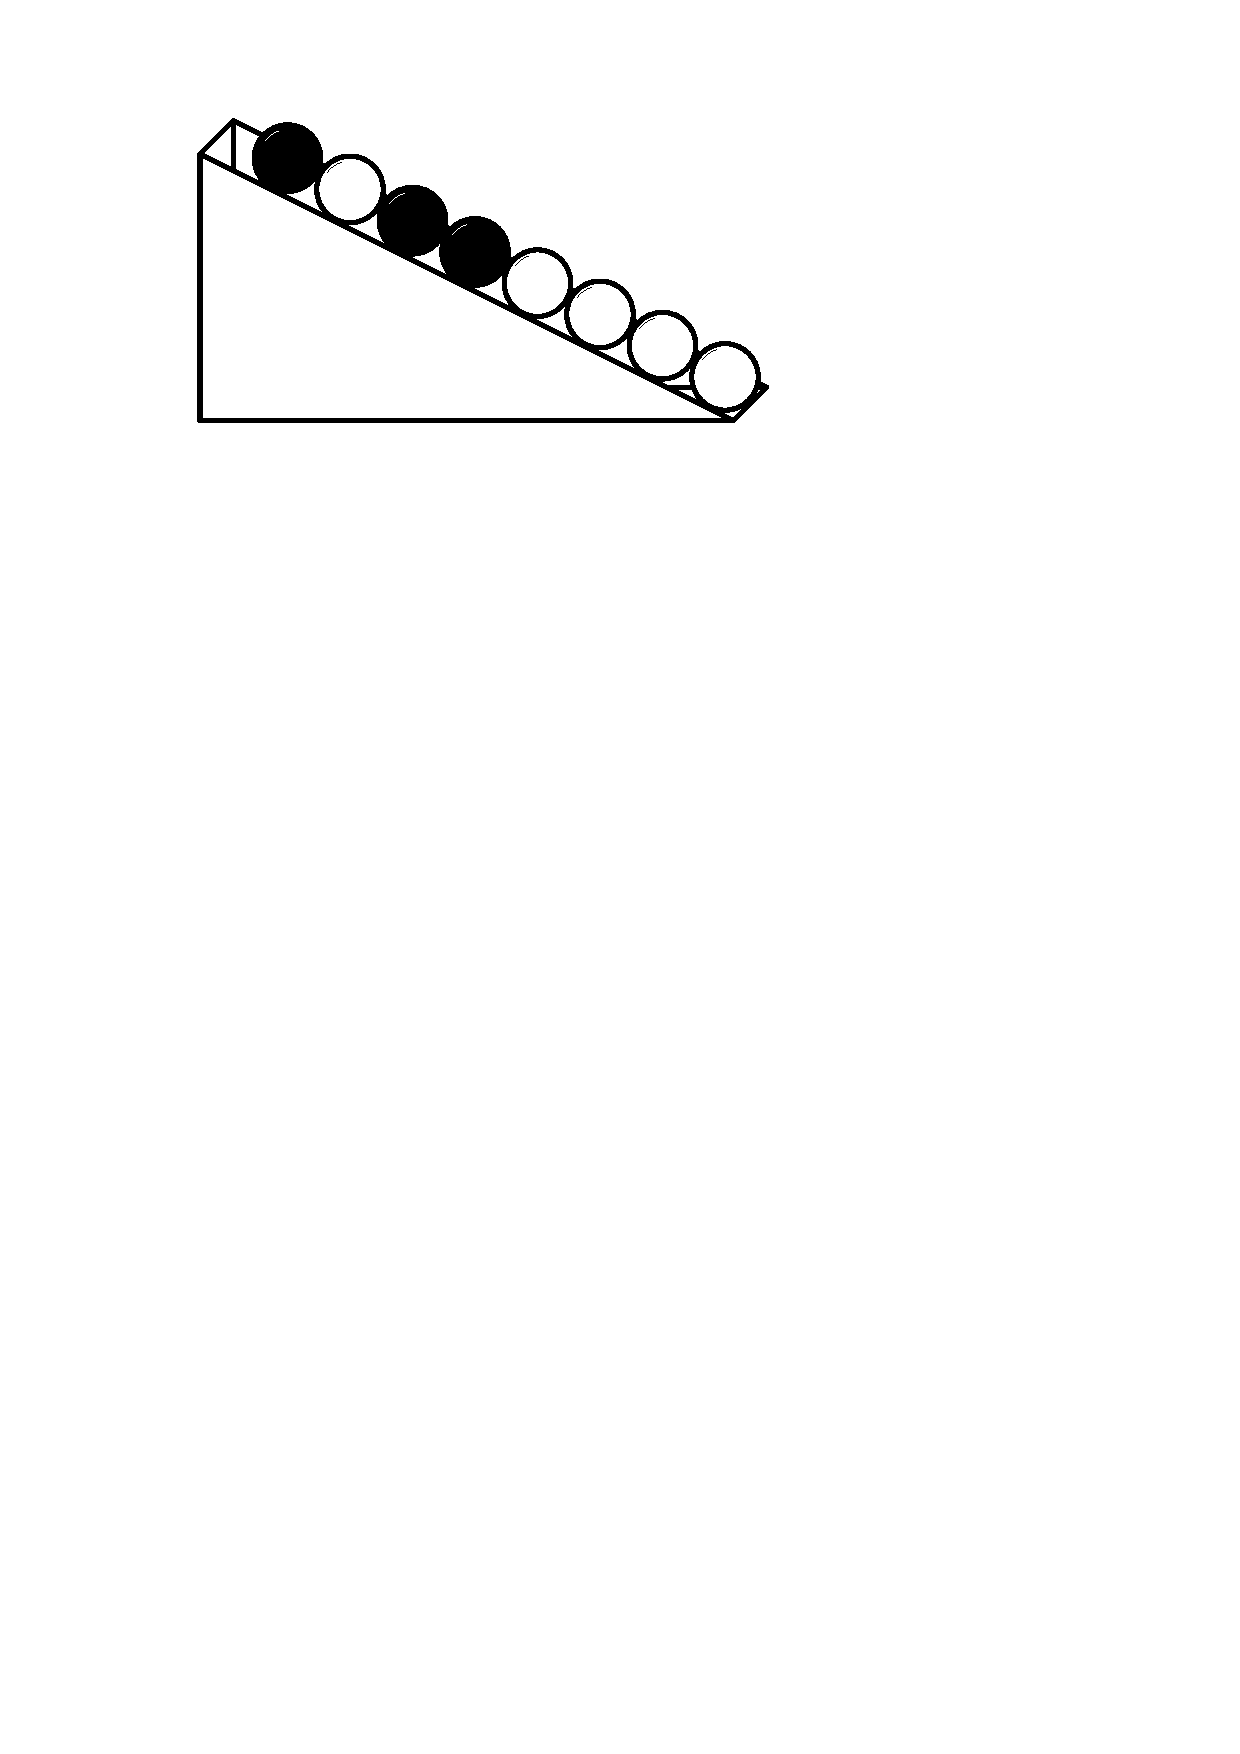
\includegraphics[width=.3\textwidth]{figures/marbles_second.pdf} 

Now, consider performing the same move again: finding $x$, the first black marble that follows a white marble, and moving marble $x+1$ to the top of the ramp. This yields a third configuration.

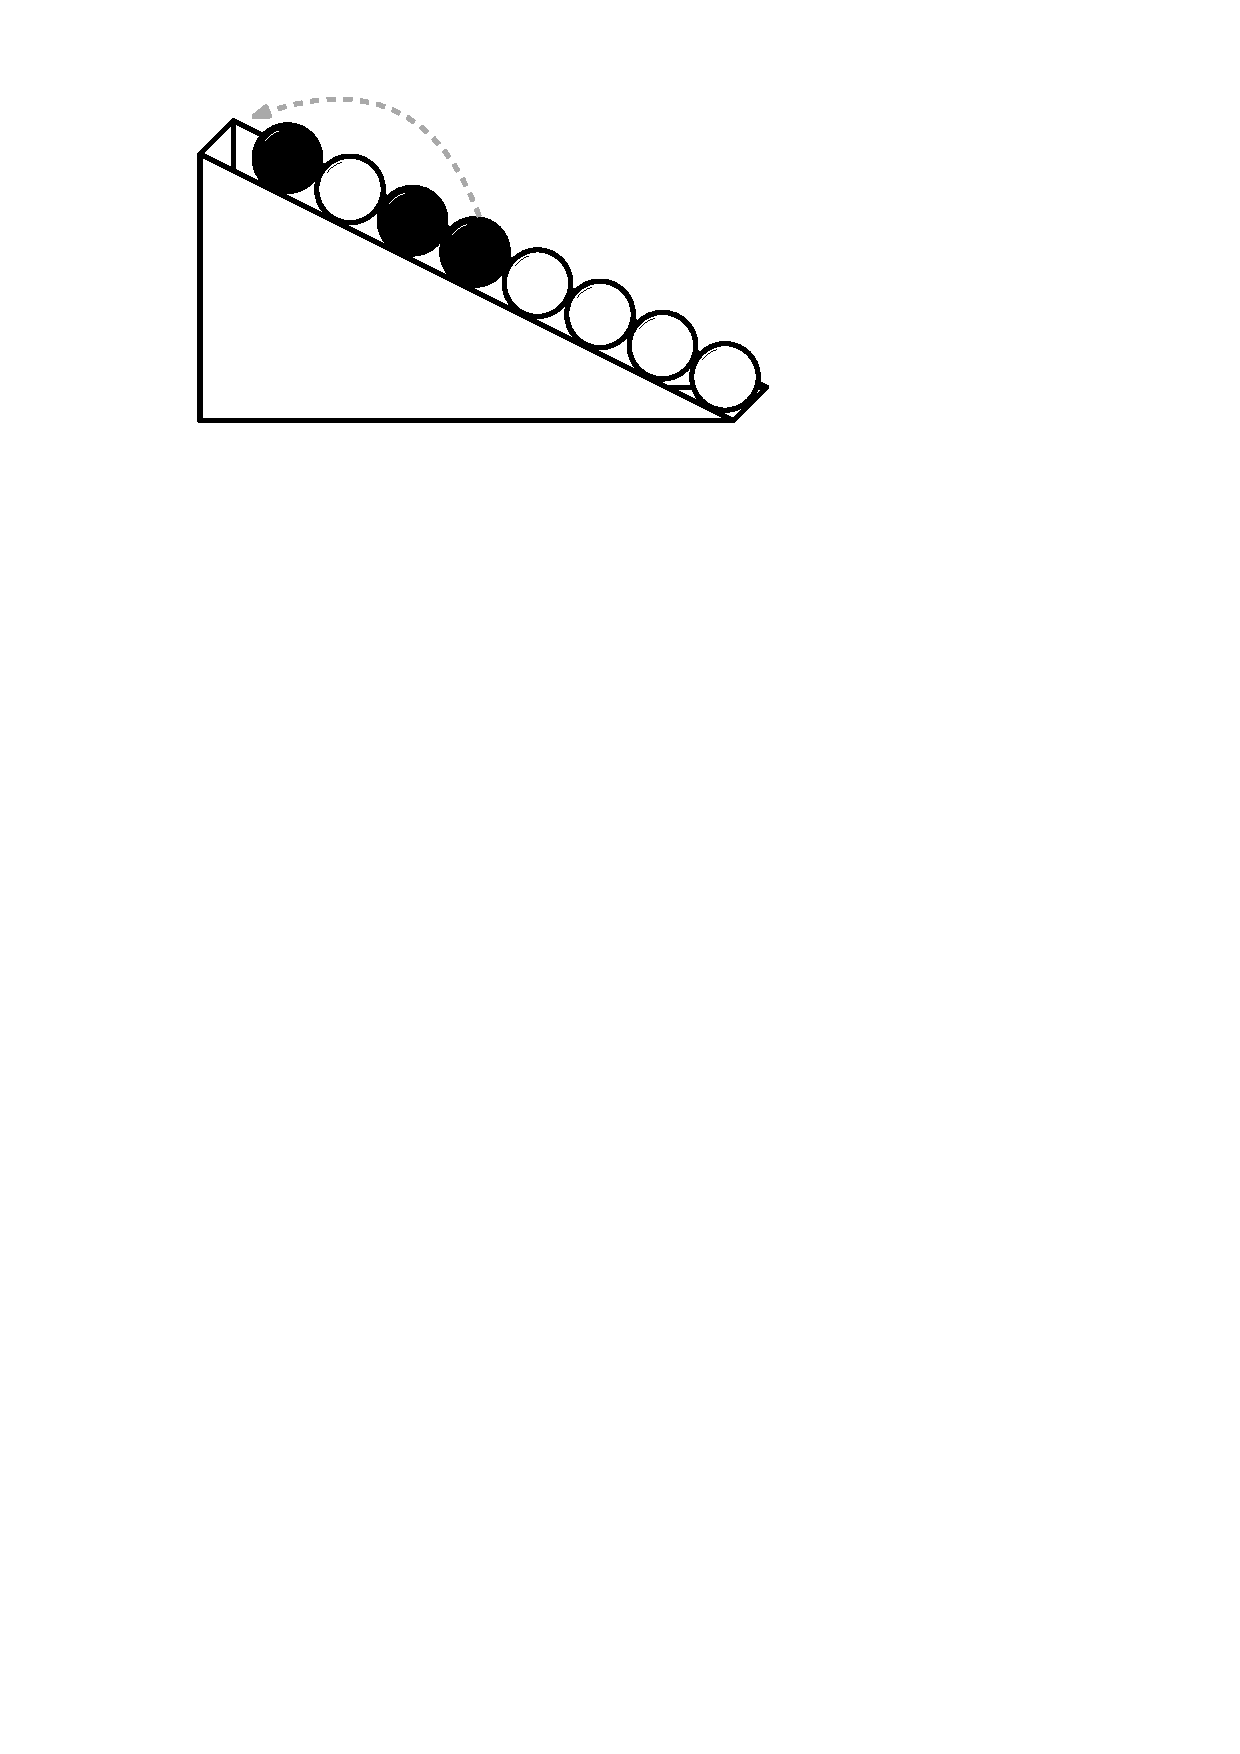
\includegraphics[width=.3\textwidth]{figures/marbles_second_arrow.pdf} $\implies$
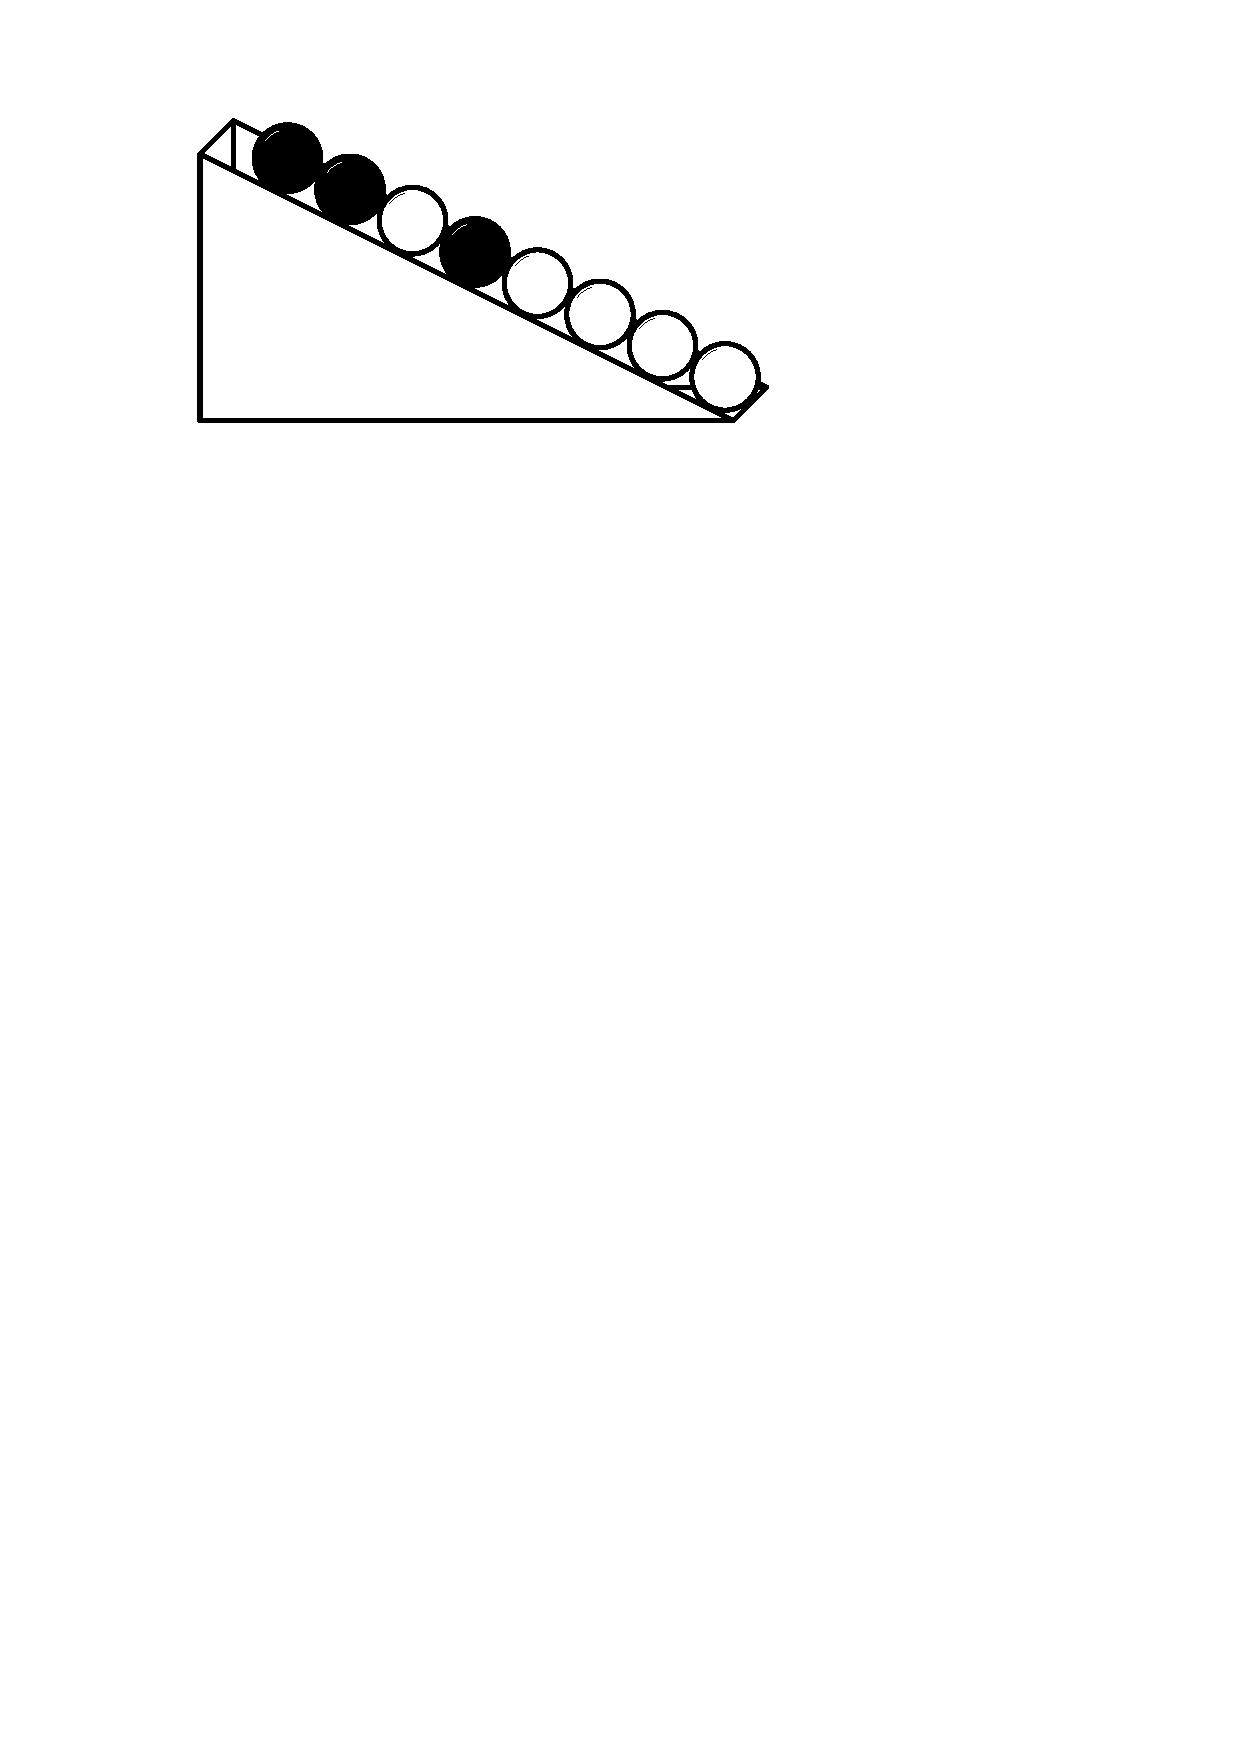
\includegraphics[width=.3\textwidth]{figures/marbles_third.pdf} 

Amazingly, repeatedly performing this operation will eventually generate all possible marble arrangements (with no distinction made between individual black and white marbles). To make the order cyclic, add an additional rule for the case where no black marble follows a white marble (all black marbles come before all white marbles).  In this case, shift the last marble to the top of the ramp.

This rule for marbles on a ramp can be translated to binary strings to create a successor rule that generates all binary strings with fixed content.  We refer to this operation of moving a single marble to the top of the ramp as a \emph{left-shift}.
The order described by this rule is 
cool-lex order, a variation of co-lexicographic order that was first introduced for $(s,t)$-combinations by Ruskey and Williams \cite{ruskey2005generating} \cite{ruskey2008generating}.  It was initially discovered by thinking about simple iterative successor rules like the successor rule for the binary reflected Gray code in equation \ref{eq:BRGC-rule}. To generate all binary strings of a given length instead of all binary strings with a fixed set of content, one only needs to change the rule slightly.  In the case where there is no black marble following a white marble, move the last marble to the top of the ramp and change its color.  In binary strings, this rule corresponds to left-shifting the last bit to the front of the string and complementing it.

Cool-lex order has some advantages of both lexicographic orderings and Gray codes.  Like lexicographic orders, cool-lex order has a simple recursive structure that is easy to understand at  high level.  
Like the binary reflected Gray code, cool-lex orders often lead to generation algorithms that are simpler and more efficient than lexicographic orders.  Accordingly, cool-lex objects for exhaustively generating different sets are not just of theoretical interest.
For example, the ``multicool" package in R uses a loopless cool-lex algorithm to efficiently enumerate multiset permutations.   The package started using cool-lex order for multiset permutations in version 1.1 and as of version 1.12 has been downloaded nearly a million times \cite{multicool_2021}.  Moreover, due to its efficiency and simplicity, Don Knuth included the cool-lex algorithm for combinations in his 4th volume of \emph{The Art of Computer Programming} and provided an implementation of it for his theoretical MMIX processor architecture due to its efficiency and simplicity \cite{knuth2015art}.  Additionally, a hardware implementation of the cool-lex order for combinations in a FPGA was introduced during Madeline Burbage's award winning ACM student research presentation \cite{burbage2020cool}.

% In addition to these, applications of cool-lex order are rapidly growing and new cool-lex algorithms are being discovered every year.  




\subsection{Cool-Lex Sublists}

Like the binary reflected Gray code, cool-lex order has also been used to create additional minimal change orders via taking sublists. In particular, a binary \emph{bubble language} is a set of binary strings with the closure property that the first $01$ of any string can be replaced by $10$ to obtain another string in th set.  Ruskey, Sawada, and Williams found that all binary \emph{bubble languages} appear in a Gray code order when listed in cool-lex order.  Specifically, any binary bubble language can be listed in cool-lex order such that successive strings differ by one or two transpositions.  The approach used in this paper is similar to that discussed in \cite{sawada2021inside} for generating Gray codes for ``flip-swap" languages.  A Gray code can be obtained for any \emph{fixed weight} binary bubble language, or a binary bubble language that is a subset of $(s,t)$-combinations, by generating all $(s,t)$-combinations and filtering to contain strings in the relevant language.  Gray codes for bubble languages of varying weights can be obtained by concatenating fixed weight binary bubble language Gray codes together.
Importantly, although this approach initially involves generating a superset of a language and filtering, careful analysis of the filtered order can typically yield a direct successor rule that efficiently generates only strings in the language without filtering.  This has allowd for different versions of cool-lex order to efficiently enumerate Dyck words and binary trees \cite{ruskey2008generating}, k-ary Dyck words, \cite{durocher2012cool}, and fixed-density necklaces and other languages \cite{sawada2009fixed}.  

In addition to the cool-lex order for $(s,t)$-combinations and bubble languages, cool-lex order has been generalized to enumerate other languages as well.  In particular, cool-lex order for all binary strings of a given length \cite{stevens2012coolest} and multiset permutations \cite{williams2009loopless} have been developed as well.  Our result in Chapter \ref{chap:luka-graycode} will provide a Gray code for a subset of multiset permutations in cool-lex order that was obtained initially by filtering the cool-lex order for multiset permutations.  The resulting rule generates fixed-content Lukasiewicz words using one left-shift per generated string.


\section{Gray Codes for Trees and Catalan Objects} \label{sec:intro_Graycodes}

This thesis aims to create efficient minimal change orderings for other objects, namely ordered trees and Lukasiewicz words.  Ordered trees and Lukasiewicz words are both \emph{Catalan objects}.  The number of Lukasiewicz words of length $n+1$ and the number of ordered trees with $n+1$ nodes are both counted by the $n\thh$ Catalan number $\C_n$.  

Frank Gray's reflected binary code used complementing a single bit as the minimal change between successive binary strings in its ordering.  Other notions of minimal changes in strings are \emph{adjacent-transpositions}, or \emph{swaps}, which interchange two adjacent symbols in a string, and \emph{shifts}, in which a single symbol in a string moved to another position. Lukasiewicz words are typically represented as strings of integers, and therefore can make use of these minimal change string operations.  Our Gray codes for Lukasiewicz words will use a slightly more restrictive type of shift, a \emph{left-shift}, which moves a single symbol somewhere to the left within a string. 



% PICTURE? ESA IMAGE? BUT WITHOUT STACK?

Defining minimal changes for trees is more complicated, as what changes are \emph{minimal} within a tree is often representation dependent.  Our Gray code for ordered trees aims to use simple operations that are minimal for most reasonable tree representations.  These minimal changes use ``pops", which remove a node's first child, and ``pushes,'' which push one node to be the first child of another.  More specifically, the algorithm will generate trees using a pop-push operation that pops one node's first child and pushes it to become the first child of another node.  We will refer to this pop-push operation as a ``pull.''

% TODO: picture



\section{Goals and Results}


This thesis has the broad goal of extending cool-lex order to new objects.  It provides two primary contributions, each with sub-contributions.  

The first contribution is a `pop-push' Gray code for enumerating ordered trees in $O(1)$ time. Chapter \ref{chap:otree-graycode} will give a two-case successor rule for generating all ordered trees with $n$ nodes using at most two ``pull'' operations. Chapter \ref{chap:otree-implementation} will provide a loopless algorithm for the successor rule in \ref{chap:otree-graycode} and an implementation of the algorithm in C.  This algorithm is an extension of the cool-lex order for Dyck words and binary trees presented by Ruskey and Williams. It shows that the cool-lex order for Dyck words is simultaneously a Gray code for a third Catalan object: ordered trees, as well as Dyck words and binary trees.  These results have been submitted to an international algorithms conference and are currently under review \cite{lapeypush}.

The second contribution is a shift Gray code for Lukasiewicz words.  Lukasiewicz words are a generalization of Dyck words that allow for broader sets of content while maintining a notion of ``balance." Chapter \ref{chap:luka-graycode} will give a shift Gray code for generating Lukasiewicz words with fixed content using one prefix shift per iteration.  Chapter \ref{chap:luka-implementation} will give a loopless implementation of the algorithm in \ref{chap:luka-graycode} using an array based implementation for the special case of Motzkin words and a linked list implementation for the general case of unrestricted Lukasiewicz words.  These results have been accepted at the 33rd International Workshop on Combinatorial Algorithms and will be presented June 2022 \footnote{Although these results are presented after the ordered trees result in this paper, these results were developed earlier and therefore were submitted to an earlier conference} \cite{lapey2022shift}.

Chapter \ref{chap:catalan} will give background information on the Catalan numbers and their relation to the combinatorial objects generated by this thesis.  Chapter \ref{chap:cool} will give background information on existing applications of cool-lex order.  Chapters \ref{chap:otree-graycode} and \ref{chap:otree-implementation} will give a new successor rule and loopless implementation for generating ordered trees in cool-lex order.  Chapter \ref{chap:luka-background} will give background information on generalizations of Dyck words, including Lukasiewicz words and Motzkin words. Chapters \ref{chap:luka-graycode} and \ref{chap:luka-implementation} will give a successor rule and loopless implementation for generating fixed-content Lukasiewicz words.

The Catalan numbers are one of the most ubiquitous sequences of numbers in mathematics.  
Named for mathematician Eugene Charles Catalan, the $n\thh$ Catalan number can be succinctly defined as the number of ways of triangulating a convex polygon with $n+2$ sides.  Figure \ref{fig:pentagontriangulations} demonstrates this for the case of $n=3$ The sequence of Catalan numbers for $n \ge 0$ can be defined mathematically as follows:

\begin{align}
    \C_n &= \frac{(2n)!}{n!(n+1)!} =1, 1, 2, 5, 14, 42, 132, \ldots & \text{OEIS} A000108
\end{align}

\begin{figure}
\begin{center}
\begin{tikzpicture}
    \coordinate (a) at (-0,1);
    \coordinate (b) at (0.951,0.309);
    \coordinate (c) at (0.587,-0.809);
    \coordinate (d) at (-0.587,-0.809);
    \coordinate (e) at (-0.951,0.309);


\matrix[column sep=0.8cm,row sep=0.5cm]
{
    \pslice{a/d,a/c} &
    \pslice{b/e,b/d} &
    \pslice{c/a,c/e} &
    \pslice{d/b,d/a} &
    \pslice{e/c,e/b} \\
};
\end{tikzpicture}
\end{center}
    \caption{The $\C_3=5$ triangulations of a polygon with $3+2=5$ sides.}
\label{fig:pentagontriangulations}
\end{figure}
The Catalan numbers count a remarkable number of interesting and useful combinatorial objects in bijective correspondence with triangulations of $n$-gons. Combinatorial objects counted by the Catalan numbers are referred to as \emph{Catalan objects}.   Richard Stanley's book \emph{Catalan Numbers} gives hundreds of examples of Catalan objects  as well as a thorough history on the numbers and their study \cite{stanley2015Catalan}. This thesis will focus primarily on three Catalan objects: Dyck words, binary trees, and ordered trees. 


\section{Dyck Words and Paths} \label{sec:Dycks}

The language of binary Dyck words is the set of binary strings that satisfy the following conditions: The string has an equal number of ones and zeroes and each prefix of the string has at least as many ones as zeroes.  The number of distinct Dyck words with $n$ ones and $n$ zeroes is equal to $\C_n$.  Dyck words with $n$ ones and $n$ zeroes are frequently referred to as Dyck words of \emph{order n}.
For example, the $\C_2=2$ Dyck words of order 2 are $1100$ and $1010$.

% TODO: don't love this phrasing
Two common interpretations of Dyck words are balanced parentheses and paths in the Cartesian plane. If each one in a Dyck word is taken to represent an open parenthesis and each zero a closing parenthesis, the Dyck language becomes the language of balanced parentheses.  Alternatively, the Dyck language can be interpreted as the set of paths in the Cartesian plane using $(1,1)$ (northeast) and $(1,-1)$ (southeast) steps that start at $(0,0)$, end at $(0,0)$ and never go below the x axis. In this case, each one in a Dyck word represents a $(1,1)$ step and each zero represents a $(1,-1)$ step.

Figure $\ref{fig:Dycks}$ gives an illustration of each of these interpretations of Dyck words for $n=4$.


\begin{figure}[H]
    \centering
    % This figure is temporarily omitted because it is slow
    \begin{tabularx}{0.55\textwidth}{>{\hsize=0.4\hsize}C >{\hsize=0.2\hsize}C >{\hsize=0.2\hsize}C   }
       \thead{Dyck Path} & \thead{Dyck Word} & \thead{Parentheses} \\ \hline 
\DyckTable[1]{2,0,2,0,2,0,2,0} & 10101010 & ()()()()\\
\DyckTable[2]{2,0,2,0,2,2,0,0} & 10101100 & ()()(())\\
\DyckTable[2]{2,0,2,2,0,0,2,0} & 10110010 & ()(())()\\
\DyckTable[2]{2,0,2,2,0,2,0,0} & 10110100 & ()(()())\\
\DyckTable[3]{2,0,2,2,2,0,0,0} & 10111000 & ()((()))\\
\DyckTable[2]{2,2,0,0,2,0,2,0} & 11001010 & (())()()\\
\DyckTable[2]{2,2,0,0,2,2,0,0} & 11001100 & (())(())\\
\DyckTable[2]{2,2,0,2,0,0,2,0} & 11010010 & (()())()\\
\DyckTable[2]{2,2,0,2,0,2,0,0} & 11010100 & (()()())\\
\DyckTable[3]{2,2,0,2,2,0,0,0} & 11011000 & (()(()))\\
\DyckTable[3]{2,2,2,0,0,0,2,0} & 11100010 & ((()))()\\
\DyckTable[3]{2,2,2,0,0,2,0,0} & 11100100 & ((())())\\
\DyckTable[3]{2,2,2,0,2,0,0,0} & 11101000 & ((()()))\\
\DyckTable[4]{2,2,2,2,0,0,0,0} & 11110000 & (((())))\\
    \end{tabularx}
    \caption{The $\C_4=14$ Dyck words of order 4 in lexicographic order}
    \label{fig:Dycks}
\end{figure}
\section{Binary Trees}

Binary trees are fundamental objects in computer science, and are commonly used for searching, sorting, and storing data hierarchically. A binary tree can be defined recursively as follows: The empty set $\phi$ is a binary tree. Otherwise a binary tree has a root vertex, a left subtree, and a right subtree, where each subtree is also a binary tree. A closely related object is an \emph{extended binary tree}, which is a binary tree for which every non-leaf node has exactly two children.  

Binary trees and extended binary trees are both counted by the Catalan numbers: $\C_n$ is the number of binary trees with $n$ nodes and the number of extneded binary trees with $n$ internal nodes.  
A binary tree $b$ with $n$ nodes can be constructed from an extended binary tree $e$ with n internal nodes by removing all leaves from the extended binary tree, leaving the $n$ internal nodes as the only remaining nodes.

This process can be reversed to construct an extended binary tree with $n$ internal nodes from a binary tree with $n$ nodes. Given a binary tree $b$ with $n$ nodes, add two leaf children to every leaf in $b$ and add one leaf child to every node in $b$ with one child. Following these steps, every node originally in $b$ is now an internal node, and therefore the constructed tree is an extended binary tree with n internal nodes.

\section{Ordered Trees}

An ordered tree is a tree for which each node can have an unrestricted number of children and the order of a node's children is significant.  An ordered tree can be defined recursively as follows:


An ordered tree is a tuple $(r,C)$ where $r$ is a root node and $C$ is either the empty set $\phi$ or an ordered sequence of children $(P_1\dots P_m)$ where each $P_i$ is an ordered tree.  Because of the designation of $r$ as a root vertex, an ordered tree cannot be empty, unlike a binary tree.

The number of ordered trees with $n+1$ nodes is equal to $\C_n$.

\begin{figure}
    \begin{subfigure}[]{\textwidth}
	\centering
\begin{tikzpicture}[every tree node/.style={draw,circle},sibling distance=6, level distance=20]
\tikzset{every tree node/.style={minimum width=1.4em,draw,circle},
         blank/.style={draw=none},
         edge from parent/.style=
         {draw,edge from parent path={(\tikzparentnode) -- (\tikzchildnode)}},
         level distance=1.5cm}
    \Tree [.{} [.{} [.{} \edge[draw=none]; \node[blank]{};\edge[draw=none]; \node[blank]{};] \edge[draw=none]; \node[blank]{};] \edge[draw=none]; \node[blank]{};] 
\end{tikzpicture}
\begin{tikzpicture}[every tree node/.style={draw,circle},sibling distance=6, level distance=20]
\tikzset{every tree node/.style={minimum width=1.4em,draw,circle},
         blank/.style={draw=none},
         edge from parent/.style=
         {draw,edge from parent path={(\tikzparentnode) -- (\tikzchildnode)}},
         level distance=1.5cm}
    \Tree [.{} \edge[draw=none]; \node[blank]{};[.{} [.{} \edge[draw=none]; \node[blank]{};\edge[draw=none]; \node[blank]{};] \edge[draw=none]; \node[blank]{};] ] 
\end{tikzpicture}
\begin{tikzpicture}[every tree node/.style={draw,circle},sibling distance=6, level distance=20]
\tikzset{every tree node/.style={minimum width=1.4em,draw,circle},
         blank/.style={draw=none},
         edge from parent/.style=
         {draw,edge from parent path={(\tikzparentnode) -- (\tikzchildnode)}},
         level distance=1.5cm}
    \Tree [.{} [.{} \edge[draw=none]; \node[blank]{};[.{} \edge[draw=none]; \node[blank]{};\edge[draw=none]; \node[blank]{};] ] \edge[draw=none]; \node[blank]{};] 
\end{tikzpicture}
\begin{tikzpicture}[every tree node/.style={draw,circle},sibling distance=6, level distance=20]
\tikzset{every tree node/.style={minimum width=1.4em,draw,circle},
         blank/.style={draw=none},
         edge from parent/.style=
         {draw,edge from parent path={(\tikzparentnode) -- (\tikzchildnode)}},
         level distance=1.5cm}
    \Tree [.{} \edge[draw=none]; \node[blank]{};[.{} \edge[draw=none]; \node[blank]{};[.{} \edge[draw=none]; \node[blank]{};\edge[draw=none]; \node[blank]{};] ] ] 
\end{tikzpicture}
\begin{tikzpicture}[every tree node/.style={draw,circle},sibling distance=6, level distance=20]
\tikzset{every tree node/.style={minimum width=1.4em,draw,circle},
         blank/.style={draw=none},
         edge from parent/.style=
         {draw,edge from parent path={(\tikzparentnode) -- (\tikzchildnode)}},
         level distance=1.5cm}
    \Tree [.{} [.{} \edge[draw=none]; \node[blank]{};\edge[draw=none]; \node[blank]{};] [.{} \edge[draw=none]; \node[blank]{};\edge[draw=none]; \node[blank]{};] ] 
\end{tikzpicture}

	\caption{The $\C_3=5$ binary trees with 3 nodes}
	\label{fig:binarytrees}
	\label{fig:}
    \end{subfigure}
    \begin{subfigure}[]{\textwidth}
	\centering
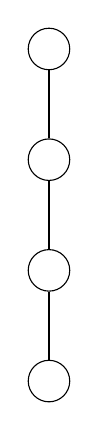
\begin{tikzpicture}[every tree node/.style={draw,circle},sibling distance=10pt, level distance=40pt]
\tikzset{minimum width=1.5em,edge from parent/.style={draw, edge from parent path=
    {(\tikzparentnode) -- (\tikzchildnode)}}}
    \Tree [.{} [.{} [.{} [.{} ] ] ] ] 
\end{tikzpicture} \hspace{2.9em}
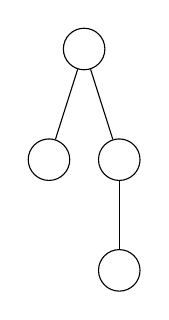
\begin{tikzpicture}[every tree node/.style={draw,circle},sibling distance=10pt, level distance=40pt]
\tikzset{minimum width=1.5em,edge from parent/.style={draw, edge from parent path=
    {(\tikzparentnode) -- (\tikzchildnode)}}}
    \Tree [.{} [.{} ] [.{} [.{} ] ] ] 
\end{tikzpicture} \hspace{2.9em}
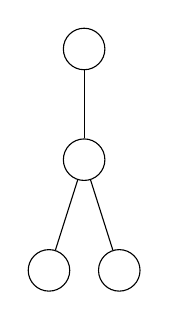
\begin{tikzpicture}[every tree node/.style={draw,circle},sibling distance=10pt, level distance=40pt]
\tikzset{minimum width=1.5em,edge from parent/.style={draw, edge from parent path=
    {(\tikzparentnode) -- (\tikzchildnode)}}}
    \Tree [.{} [.{} [.{} ] [.{} ] ] ] 
\end{tikzpicture} \hspace{2.9em}
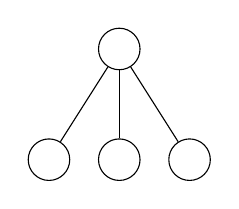
\begin{tikzpicture}[every tree node/.style={draw,circle},sibling distance=10pt, level distance=40pt]
\tikzset{minimum width=1.5em,edge from parent/.style={draw, edge from parent path=
    {(\tikzparentnode) -- (\tikzchildnode)}}}
    \Tree [.{} [.{} ] [.{} ] [.{} ] ] 
\end{tikzpicture} \hspace{2.9em}
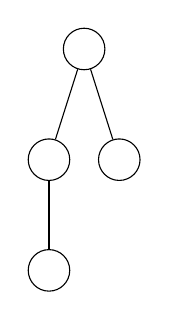
\begin{tikzpicture}[every tree node/.style={draw,circle},sibling distance=10pt, level distance=40pt]
\tikzset{minimum width=1.5em,edge from parent/.style={draw, edge from parent path=
    {(\tikzparentnode) -- (\tikzchildnode)}}}
    \Tree [.{} [.{} [.{} ] ] [.{} ] ] 
\end{tikzpicture}
	\caption{The $\C_3=5$ ordered trees with $3+1=4$ nodes}
	\label{fig:otrees}
    \end{subfigure}
\end{figure}



\section{Bijections}

Since Dyck Words, binary trees, and ordered trees are all Catalan objects, all three sets of objects are in bijective correspondence with each other.  For convenience, we will use the $\mathbf{D}_n$, $\mathbf{B}_n$, $\mathbf{E}_n$, and $\mathbf{T}_n$ to refer to the set of Dyck words of order $n$, the set of binary trees with $n$ nodes, the set of extended binary trees with $n$ internal nodes, and the set of ordered trees with $n+2$ nodes respectively.  

\subsection{Binary Trees and Dyck Words}

The bijection between extended binary trees and Dyck words is particularly elegant: 
For any $e \in \mathbf{E}_n$, traverse e in preorder.  Record a $1$ for each internal node; record a $0$ for each leaf ignoring the final leaf. The resulting binary sequence is a Dyck word  $D \in \mathbf{D}_n $ corresponding to the extended binary tree $e$.  This process can be reversed to go from $\mathbf{D}_n$ to $\mathbf{E}_n$.

\begin{figure}
    \centering
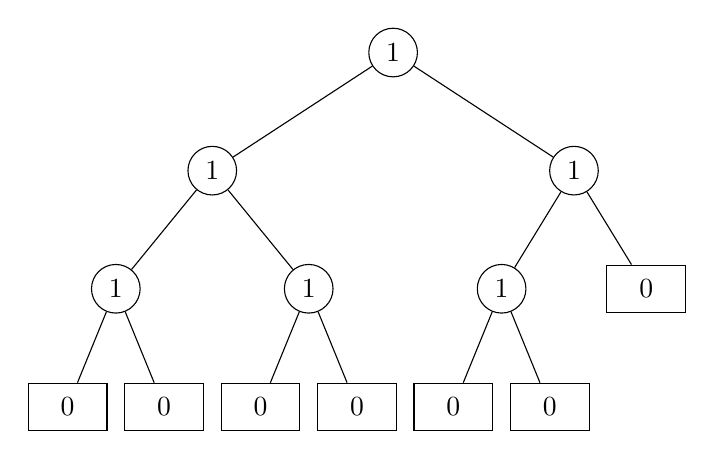
\begin{tikzpicture}[every tree node/.style={draw,circle},sibling distance=6, level distance=20]
\tikzset{every tree node/.style={minimum width=1.5em,draw,circle},
         blank/.style={draw=none},
         edge from parent/.style=
         {draw,edge from parent path={(\tikzparentnode) -- (\tikzchildnode)}},
         level distance=1.5cm}
    \Tree [.{1} [.{1} [.{1} [.\node[style={rectangle,minimum height=.6cm,minimum width=1cm}]{0}; ][.\node[style={rectangle,minimum height=.6cm,minimum width=1cm}]{0}; ]] [.{1} [.\node[style={rectangle,minimum height=.6cm,minimum width=1cm}]{0}; ][.\node[style={rectangle,minimum height=.6cm,minimum width=1cm}]{0}; ]] ] [.{1} [.{1} [.\node[style={rectangle,minimum height=.6cm,minimum width=1cm}]{0}; ][.\node[style={rectangle,minimum height=.6cm,minimum width=1cm}]{0}; ]] [.\node[style={rectangle,minimum height=.6cm,minimum width=1cm}]{0}; ]] ] 
\end{tikzpicture} \hspace{1em}
\begin{tikzpicture}[every tree node/.style={draw,circle},sibling distance=6, level distance=20]
\tikzset{every tree node/.style={minimum width=1.5em,draw,circle},
         blank/.style={draw=none},
         edge from parent/.style=
         {draw,edge from parent path={(\tikzparentnode) -- (\tikzchildnode)}},
         level distance=1.5cm}
    \Tree [.{} [.{} [.{} \edge[draw=none]; \node[blank]{};\edge[draw=none]; \node[blank]{};] [.{} \edge[draw=none]; \node[blank]{};\edge[draw=none]; \node[blank]{};] ] [.{} [.{} \edge[draw=none]; \node[blank]{};\edge[draw=none]; \node[blank]{};] \edge[draw=none]; \node[blank]{};] ] 
\end{tikzpicture}
    \caption{The extended binary tree (left) and binary tree (right) corresponding to the Dyck word 111001001100 \\
    Note that a preorder traversal of the extended binary tree excluding its final leaf yields 111001001100.
    }
\label{fig:binarytreesbijection}
\end{figure}


\subsection{Ordered Trees and Dyck Words} \label{subsec:otree-dyck-bij}
The bijection between ordered trees and Dyck words is particularly relevant to this paper's results, as it is central to the loopless ordered tree generation algorithm given in Chapter \ref{chap:otree-graycode}.
This algorithm will use the bijection between ordered trees and Dyck words specified in Richard Stanley's \emph{Catalan Objects} \cite{stanley2015Catalan}. Figure \ref{ordered_tree_bijection_illustration} illustrates both directions of the bijection.
The bijection can be formalized as follows:
\footnote{ Stanley's text refers to ordered trees as \emph{plane trees} and Dyck words as \emph{ballot sequences}} 


Given an ordered tree T with $n+1$ nodes: Traverse T in preorder.  Whenever going ``down" an edge, or away from the root, record a 1.  Whenever going ``up" an edge, or towards the root, record a 0.  The resulting binary sequence is a Dyck word D corresponding to the ordered tree T. 

This process can be inverted as follows: 

Let $D=d_1...d_{2n}$ be a Dyck word of order $n$ with $n > 0$. Construct an ordered tree T via the following steps. 

Let T be an ordered tree with root $r$.  Keep track of a current node $c$ and set $c$ equal to the root $r$.

\begin{itemize}
    \item For each $d_i$ such that $1 \le i \le 2n$ 
	\begin{itemize}
	    \item if $d_i=1$, then add a rightmost child $ch$ to $c$'s children; set $c=ch$
	    \item if $d_i=0$, then set $c$ equal to $c$'s parent.
	\end{itemize}
	%TODO: QUESTION: do I need to prove this? It seems like Stanely assumed this was basically obvious 

\end{itemize}

Following the execution of these steps, $r$ is the root of an ordered tree with $n$ nodes corresponding to the Dyck word $D$.

\begin{figure}
    \centering
    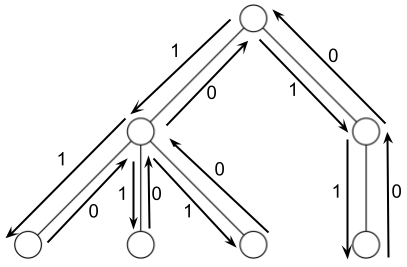
\includegraphics[width=0.5\textwidth]{otreebij.png}
    \caption{An ordered tree with $6+1=7$ nodes corresponding to the order 6 Dyck word $110101001100$.}
    \label{ordered_tree_bijection_illustration}
\end{figure}

\section{Minimal Changes}
Much of this thesis's content concerns minimal change orderings for Catalan objects.  Notably, our notion of a minimal change must differ for different Catalan objects: a minimal change between two Catalan objects of one type will not necessarily correspond to a minimal change between two Catalan objects of a different type.  Figure \ref{fig:badminimalchange} gives an example where a single bit transposition in a Dyck word results in updating worst-case $O(n)$ nodes in an ordered tree.  This makes the goal of creating an ordering that is a Gray code for multiple different combinatorial objects difficult, as it has to be a minimal change ordering for each object being generated.  We refer to orderings that are Gray codes for multiple combinatorial objects as \emph{simultaneous Gray codes}.  Ruskey and Williams showed that the cool-lex order for Dyck words is a simultaneous Gray code for Dyck words and binary trees \cite{ruskey2008generating}.  Another example of a simultaneous Gray code is the TODO: name? simultaneous Gray code for Baxter permutations and rectangulations given by (Hartung and Merino?) \cite{hartung2020combinatorial} \cite{merino2021efficient}.  Chapter \ref{chap:otree-graycode}, we show that the cool-lex order for Dyck words and binary trees is also a Gray code for Ordered trees, thus completing a single Gray-code ordering for three of the most important Catalan structures.

\begin{figure}[]

    \centering

    \textbf{\textcolor{midpurp}{1101010}}\textbf{\textcolor{red}{10}}\textbf{\textcolor{OliveGreen}{1010100}}

    $\implies$

    \textbf{\textcolor{midpurp}{1101010}}\textbf{\textcolor{red}{01}}\textbf{\textcolor{OliveGreen}{1010100}}
        

\begin{tikzpicture}[every tree node/.style={draw,circle},sibling distance=10pt, level distance=40pt]
\tikzset{minimum width=1.25em,edge from parent/.style={draw, edge from parent path=
    {(\tikzparentnode) -- (\tikzchildnode)}}}
    \Tree [.\node[style={fill=none}]{}; [.\node[style={fill=lmidpurp}]{}; [.\node[style={fill=lmidpurp}]{}; ] [.\node[style={fill=lmidpurp}]{}; ] [.\node[style={fill=lmidpurp}]{}; ] 
    [.\node[style={fill=lightred}]{}; ] 
    [.\node[style={fill=midishgreen}]{}; ] [.\node[style={fill=midishgreen}]{}; ] [.\node[style={fill=midishgreen}]{}; ] ] ] 
\end{tikzpicture} $\implies$
\begin{tikzpicture}[every tree node/.style={draw,circle},sibling distance=10pt, level distance=40pt]
\tikzset{minimum width=1.25em,edge from parent/.style={draw, edge from parent path=
    {(\tikzparentnode) -- (\tikzchildnode)}}}
    \Tree [.\node[style={fill=none}]{}; [.\node[style={fill=lmidpurp}]{}; [.\node[style={fill=lmidpurp}]{}; ] [.\node[style={fill=lmidpurp}]{}; ] [.\node[style={fill=lmidpurp}]{}; ] ] [.\node[style={fill=lightred}]{}; 
    [.\node[style={fill=midishgreen}]{}; ] [.\node[style={fill=midishgreen}]{}; ] [.\node[style={fill=midishgreen}]{}; ] ] ] 
\end{tikzpicture}

        \caption{A single bit transposition in a Dyck word resulting in an ordered tree change that would require updating several pointers in a link-based representation.\\
        In particular, if this example were generalized to the case where the initial Dyck word is 
        $1(10)^n0$, the corresponding ordered tree's first non-root node will have $n$ children.  In that case, transposing bits $n+1$ and $n+2$ in the Dyck word would require updating at least $n/2$ pointers in a link-based tree representation.
        }
        \label{fig:badminimalchange}
\end{figure}


\section{Recursive Enumeration}

To gain more insight into Catalan objects, we conclude this chapter by considering an alternate formula for enumerating the Catalan objects and illustrate the formula for several specific objects.

The Catalan numbers can also be expressed through a summation that hints at the recursive structure of many of the Catalan objects.  

\begin{align}
    \C_{n+1} &= \sum_{k=0}^{n}{\C_{k}\C_{n-k}} \textrm{,   }  \C_0=1
\end{align} 

In the case of triangulated polygons, this summation can be derived as follows:

$\C_{n+1}$ is the way of triangulating a convex polygon with $n+3$ sides.  Let $\mathcal{P}_{n+3}$ be a convex $(n+3)$-gon and let $\mathcal{T}$ be a triangulation of $\mathcal{P}_{n+3}$. Fix an edge $e$ in $\mathcal{P}_{n+3}$.  Note that $e$ lies between two vertices of $\mathcal{P}_{n+3}$. $e$ must be in exactly one triaingle in $\mathcal{T}$.  Let $T_{i}$ be the triangle in $\mathcal{T}$ that contains $e$.  $T_{i}$ must have two of its vertices on the two vertices of $e$ and one vertex that is another vertex in $\mathcal{P}_{n+3}$.  There are $n+1$ other vertices of $\mathcal{P}_{n+3}$.  Suppose the third vertex of $T_i$ is $k+1$ vertices clockwise of $e$, where $0\le k \le n$. Drawing $T_i$ divides $\mathcal{P}_{n+3}$ into 3 polygons: $T_i$, a $(k+2)$-gon clockwise of $T_i$, and a $(n-k+2)$-gon counterclockwise of $T_i$. This means that for each possible value of k, there is one way of triangulating $T_i$, $\C_k$ ways of triangulating the polygon clockwise of $T_i$, and $\C_{n-k}$ ways of triangulating the polygon counterclockwise of $T_i$.  Therefore, there are $C_k*C_{n-k}$ ways of triangulating $\mathcal{P}_{n+3}$ for each value of k.  Therefore, there are $\C_{n+1}=\sum_{k=0}^{n}{\C_{k}\C_{n-k}}$ total ways of triangulating $\mathcal{P}_{n+3}$. Figure \ref{fig:recursiveTriangulations} illustrates this process for the case of $n+1=6$.

\begin{figure}
    \centering
\begin{center}
\begin{tabular}{ c c c c c c c}
    $k=0$ & $k=1$ & $k=2$&$k=3$& $k=4$& $k=5$& \\
    \octoSliceTableD & \octoSliceTableC  & \octoSliceTableB  & \octoSliceTableA & \octoSliceTableH  & \octoSliceTableG   \\
    $\dycksplit{0}{5}$ & $\dycksplit{1}{4}$ & $\dycksplit{2}{3}$ & $\dycksplit{3}{2}$& $\dycksplit{4}{1}$& $\dycksplit{5}{0}$\\
    2-gon; 7-gon & 3-gon; 6-gon& 4-gon; 5-gon&5-gon; 4-gon & 6-gon; 3-gon& 7-gon; 2-gon& \\
    $\textcolor{catleft}{\C_0} *\textcolor{catright}{\C_5}$ & $\textcolor{catleft}{\C_1} *\textcolor{catright}{\C_4}$&$\textcolor{catleft}{\C_2} *\textcolor{catright}{\C_3}$ & $\textcolor{catleft}{\C_3} *\textcolor{catright}{\C_2}$&$\textcolor{catleft}{\C_4} *\textcolor{catright}{\C_1}$ & $\textcolor{catleft}{\C_5} *\textcolor{catright}{\C_0}$ \\

    $1 *42$ & $1 * 14$&$2*5$ & $5*2$&$14*1$ & $42*1$ \\
    $42$ & $14$ & $10$ & $10$ & $14$ & $42$
\end{tabular}

\bigskip


$C_6=\sum_{k=0}^5\C_k\C_{n-k}=42 + 14 + 10 + 10 + 14 + 42 = 132$
\end{center}
    \caption{Constructing $\C_6$ recursively using polygons and Dyck words. \\
    In the case of triangulated polygons, the blue region is a polygon with $k+2$ sides, the gray region is a triangle, and the red region is a polygon with $n-k+2$ sides.  The blue region can be triangulated $\C_k$ ways, the gray region is already a triangle and therefore can be triangulated 1 way, and the red region can be triangulated $C_{n-k}$ ways. Note again the special case of $k=0$ or $n-k=0$.  We define a 2-gon as having one triangulation, so $C_{0}=0$ \\
    In the case of Dyck words, each $\{\D_i\}$ can expand to any of the $\C_i$ Dyck words of order $i$.  Thus, the expression $(\{\D_k\})\{\D_{n-k}\}$ has $\C_{k}*\C_{n-k}$ possible expansions.  Note that we define $\D_0$ as having only one possible expansion, the empty string.
}
    \label{fig:recursiveTriangulations}
\end{figure}

This chapter will give background information on cool-lex order and the sets it has been used to enumerate.  
\section{Combinations: Fixed-Weight Binary Strings} \label{sec:coolCombo}
Generating all binary strings with $s$ zeroes and $t$ ones is often referred to as combinations, since each string can be used to represent a choice of $t$ elements from a set of size of $s+t$.  The cool-lex successor rule for generating all fixed-weight binary strings was given by Aaron Williams in his Ph. D thesis and is as follows \cite{williams2009shift}:

\noindent Let $\alpha$ be a binary string of length $n$.

\noindent Let $y$ be the position of the leftmost zero in $\alpha$ and $x$ be the position of the leftmost 1 in $\alpha$ such that $x > y$.  If there is no such 1, let $x=n$.

\noindent Note that $\alpha_1...\alpha_{x-1}$ is the non-increasing prefix of $\alpha$.

\noindent Let $\leftshift[\alpha]{i}$ be a simplified version of the left shift function defined in equation \ref{eq:leftdef}:  $\leftshift[\alpha]{i}$ shifts the $i\thh$ symbol of $\alpha$ into the first position.  Thus, $\leftshift[\alpha]{i}=\lshiftindex[\alpha]{1}{i}$.

% function that shifts the $i\thh$ bit of $\alpha$ into the rotates the first i bits of a string $\alpha$ right circularly by one.

% More formally, 
% \noindent $\leftshift[\alpha]{i}=\alpha_2,\alpha_3,...,\alpha_i,\alpha_1,\alpha_{i-1},\alpha_{i+1},\alpha_{i+2},...,\alpha_{2n}$
\begin{equation*}
    \overleftarrow{\text{cool}}(\alpha) = \begin{cases}
	\leftshift[\alpha]{x} & \text{if $\alpha_{x+1}=1$}\\
	\leftshift[\alpha]{x+1} & otherwise\\
\end{cases}
\end{equation*}

Note that $\alpha_1...\alpha_{x-1}$ must be exactly $1^{y-1}0^{x-y}$, where exponentiation denotes repeated symbols.  Because of this, the two left-shift operations can be replaced with can be replaced with either one or two symbol transpositions.

\noindent Let $\transpose{\alpha}{i}{j}$ with $1 \le i \le j \le n$ be a function that swaps $\alpha_i$ an $\alpha_j$.  More formally, $\transpose{\alpha}{i}{j}=\alpha_1,\alpha_2,\dots,\alpha_{i-1},\alpha_{j}\alpha_{i+1}\dots \alpha_{j-1}\alpha_i \alpha_{j+1}\dots \alpha_n$
The left-shift rule can be re-stated as follows:

\begin{equation*}
    \overleftarrow{\text{cool}}(\alpha) = \begin{cases}
	\transpose{\alpha}{y}{x} & \text{if $\alpha_{x+1}=1$}\\
	\transpose{\transpose{\alpha}{y}{x}}{1}{x+1} & otherwise\\
\end{cases}
\end{equation*}

% To illustrate the first case, consider $\alpha=11001101$; note that x=5. $\leftshift{5}{1}=11100101$ can be accomplished by just setting $\alpha_3=1$ and $\alpha_5=0$, or alternatively $\transpose{\alpha}{3}{5}$

% To illustrate the second case, consider $\alpha=11100101$; note that x=6. $\leftshift{7}{1}=01110011$ with on  can be accomplished by setting $\alpha_4=1$, $\alpha_6=0$, $\alpha_7=1$, and $\alpha_1=0$.  

%Equivalently, the shift can be performed by $\transpose{\transpose{\alpha}{4}{6}}{1}{7}$

% Thus, depending on the value of $\alpha_{x+1}$, the cool-lex successor rule for binary strings requires either one or two transpositions per combination.  

\section{Cool Lex Order on Dyck Paths and Binary Trees}

Ruskey and Williams found the following successor rule for enumerating binary Dyck words, dubbed ``CoolCat" due to its use of a cool-lex order to generate (cat)alan objects \cite{ruskey2008generating}:
We will use $\mathbf{D}_n$ to denote binary Dyck words with $n$ ones and $n$ zeroes.  Note that the length of any string in $\mathbf{D}_n$ is therefore $2n$.

\noindent Let $D \in \mathbf{D}_n$

\noindent Let the $i$th prefix shift of D, denoted by $\preshift{D}{i}$, be a function that rotates the second through $i\thh$ symbols of D one to the right circularly.  More formally, 

\noindent $\preshift{D}{i}=d_1,d_i,d_2,...,d_{i-1},d_{i+1},d_{i+2},...,d_{2n}$

\noindent Note that the prefix shift operation is a special case of the left shift operation defined in $\ref{eq:leftdef}$: $\preshift{D}{i}=\lshiftindex[D]{2}{i}$



\noindent Let $k$ be the index of the 1 in the leftmost $01$ substring in $D$ if it exists and $2n$ if $D$ has no $01$ substring. Note that if $D$ has no $01$ substring, then $D=1^n0^n$.
Furthermore, note that this definition of $k$ is equivalent to the definition of $x$ in \ref{sec:coolCombo}
The successor rule for $D$ is as follows:


\begin{subnumcases}{\coolCat{D} = \label{eq:prefixDyck_simple}}
	% \preshift{D}{2n} & \text{if $D$ has no $01$ substring}\\
	\preshift{D}{k+1} & if $\preshift{D}{k+1} \in \mathbf{D}_n$\\
	\preshift{D}{k} & otherwise
\end{subnumcases}

Ruskey and Williams's algorithm can also enumerate a broader set of strings: The algorithm enumerates any set $\mathbf{D}_{s,t}$ where any $D \in \mathbf{D}_{s,t}$ has s zeroes and t ones and satisfies the constraint that each prefix of D has as many ones as zeroes.  This is slightly broader than the language of Dyck words, as it does not have the requirement that a string have an equal number of ones and zeroes.
We will focus on $\mathbf{D}_n$  languages due to their correspondce with Dyck words and therefore other Catalan objects.

Evaluating whether $\preshift{D}{k+1} \in \mathbf{D}_n$ can be determined by looking at $D_{k+1}$ and the the first $k-1$ symbols of D: 

If $D_{k+1}=1$, then shifting it into the second position is valid.  If $D_{k+1}=0$ and $D$ starts with at least $\frac{k-1}{2}$ ones, then shifting a 0 into the second position will not invalidate the condition that all prefixes of $D$ have at least as many ones as zeroes.   Therefore, the successor rule in \ref{eq:prefixDyck_simple} can be simplified to the following: 

% Let $D'=$ $\preshift{D}{k+1}$

% Note that we know $D \in \mathbf{D}_n$.  

% Since preshift only rotates symbols, $D'$ will automaticallly satisfy the requirement that strings in $\mathbf{D}_n$ must have an equal number of zeroes and ones since D satisfied that requirement. Thus, $D' \in \mathbf{D}_n$ will be determined by whether or not all prefixes of $D'$ have at least as many ones as zeroes.  

% If $D_{k+1}$ is a 1, then  for all i, the $i\thh$ prefix of $D'$ will have at least as many ones as the $i\thh$ prefix of D.  Thus, $D'$ must be $\in \mathbf{D}_n$, as rotating a 1 to earlier in the string will never invalidate the requirement that every prefix of the string has at least as many ones as zeroes.  

% Note that the $k\thh$ prefix of D must be of the form $1^a0^b1$, as otherwise there would be an earlier $01$ prefix.  Fruthermore, $a\ge b$ as otherwise the bth prefix of D would have more zeroes than ones and D would not be a valid Dyck word.

% If $D_{k+1}$ is a 0, then $D' \notin \mathbf{D}_n$ if and only if rotating a 0 to index 2 creates a prefix of D with more zeroes than ones.  This will only happen if the $(k-1)\thh$ prefix of D is exactly $1^{\frac{k-1}{2}}0^{\frac{k-1}{2}}$.  

% Therefore, $\preshift{D}{k+1} \in \mathbf{D}_n \iff D_{k+1}=1$ or $D$ starts with more than $\lfloor \frac{k-1}{2} \rfloor$ ones 

\begin{subnumcases}{\coolCat{D} = \label{eq:prefixDyck}}
    % \preshift{D}{2n} & \text{if $D$ has no $01$ substring} \label{eq:prefixDyck_n}\\
	\preshift{D}{k+1} & $D_{k+1}=1$ or $D$ starts with at least $\lfloor \frac{k-1}{2} \rfloor$ ones \label{eq:prefixDyck_k1}\\
	\preshift{D}{k} & otherwise \label{eq:prefixDyck_k}
\end{subnumcases}


$\preshift{D}{k+1} \in \mathbf{D}_{n} \iff$ $D$ starts with more than $\lfloor \frac{k-1}{2} \rfloor$ ones

Ruskey and Williams provided a loopless pseudocode implementation of CoolCat that utilized this fact to enumerate any $\mathbf{D}_{s,t}$ using at most 2 conditionals per successor \cite{ruskey2008generating}. Using the bijection between Dyck words and binary trees, Ruskey and Williams also showed that their successor rule can be translated to a loopless algorithm for generating all binary trees with $n$ nodes. 

% TODO: binary trees algorithm

Due to its simplicity and efficienty, Don Knuth included the cool-lex algorithm for Dyck words in his 4th volume of \emph{The Art of Computer Programming} and also provided an implementation of it for his theoretical MMIX processor architecture \cite{knuth2015art}.

\section{Multiset Permutations}

Cool-lex order has also been shown to enumerate multiset permutations via prefix shifts.  The rule given by Williams is as follows \cite{williams2009loopless}:

\noindent Let $\alpha$ be a multiset of length $n$.

\noindent Let $i$ be the maximum value such that $\alpha_{j-1} \ge s_j$ for all $2 \le j \le i$.  In other words, $i$ is the length of the non-increasing prefix of $\alpha$.  

Recall the definition of $\leftshift[\alpha]{i}$ from section $\ref{sec:coolCombo}$

% \noindent Let $\sigma_j(\alpha)$ be a function that shifts the $i\thh$ value of $\alpha$ into the first position, or equivalently rotates the first i elements of $\alpha$ right circularly.  More formally, 

% \noindent $\sigma_j(\alpha)=\alpha_j,\alpha_1,\alpha_1,\dots,\alpha_{j-1},\alpha_{j+1},\dots,\alpha_n $

Then

\begin{equation*}
    \text{nextPerm}(\alpha) = \begin{cases}
	\leftshift[\alpha]{i+1} & \text{if $i \le n-2$ and $\alpha_{i+2} > \alpha_i$}\\
	\leftshift[\alpha]{i+2} & \text{if $i \le n-2$ and $\alpha_{i+2} \le \alpha_i$}\\
	\leftshift[\alpha]{n} & otherwise\\
\end{cases}
\end{equation*}


See Fig. \ref{fig:permutations} for an example comparison of cool-lex and lexicographic order for two multisets.

This successor rule has the convenient property of ensuring that length of the successor's non-increasing prefix is easy to find.

In particular, if $\alpha_{i+2}$ is shifted, then the length of the non-increasing prefix is either 1 if $\alpha_{i+2}\le \alpha_1$ or $i+1$ otherwise. 

Similarly, if $\alpha_{i+1}$ is shifted, then the length of the non-increasing prefix is either 1 if $\alpha_{i+1}\le \alpha_1$ or $i+1$ otherwise. 


This property allows for a loopless implementation of the successor rule, as scanning the string to find the length of the non-increasing prefix is not required.  
A similar property regarding the length of successive non-increasing prefixes will allow for a loopless implementation of the shift Gray code for Lukasiewicz words in chapter \ref{chap:luka-implementation}.

Due to the simplicity and efficiency of this rule, it is used in the ``multicool" package in R, which is used for generating multiset permutations, Bell numbers, and other combinatorial objects \cite{multicool_2021}.   Further information on the package is available here: https://www.rdocumentation.org/packages/multicool/versions/0.1-12


\begin{figure}
    \centering

\begin{tabular}{*{4}{c@{\hspace{0.2cm}}c@{\hspace{0.4cm}}}|@{\hspace{0.2cm}}c@{\hspace{0.2cm}}c}


    Cool-Lex & & Lex & & Cool-Lex & & Lex \\
    13221 & 
\begin{tikzpicture}[scale=30/100]
\fill[fill=p1col1] (0,0) rectangle (0.75,0.4);
\fill[fill=p1col3] (0.9,0) rectangle (1.65,0.9);
\fill[fill=p1col2] (1.7999999999999998,0) rectangle (2.55,0.65);
\fill[fill=p1col2] (2.6999999999999997,0) rectangle (3.4499999999999997,0.65);
\fill[fill=p1col1] (3.5999999999999996,0) rectangle (4.35,0.4);
\end{tikzpicture}
 & 11223 & 
\begin{tikzpicture}[scale=30/100]
\fill[fill=p1col1] (0,0) rectangle (0.75,0.4);
\fill[fill=p1col1] (0.9,0) rectangle (1.65,0.4);
\fill[fill=p1col2] (1.7999999999999998,0) rectangle (2.55,0.65);
\fill[fill=p1col2] (2.6999999999999997,0) rectangle (3.4499999999999997,0.65);
\fill[fill=p1col3] (3.5999999999999996,0) rectangle (4.35,0.9);
\end{tikzpicture}
 & 1432 & 
\begin{tikzpicture}[scale=30/100]
\fill[fill=p1col1] (0,0) rectangle (0.75,0.4);
\fill[fill=p1col4] (0.9,0) rectangle (1.65,1.15);
\fill[fill=p1col3] (1.7999999999999998,0) rectangle (2.55,0.9);
\fill[fill=p1col2] (2.6999999999999997,0) rectangle (3.4499999999999997,0.65);
\end{tikzpicture}
 & 1234 & 
\begin{tikzpicture}[scale=30/100]
\fill[fill=p1col1] (0,0) rectangle (0.75,0.4);
\fill[fill=p1col2] (0.9,0) rectangle (1.65,0.65);
\fill[fill=p1col3] (1.7999999999999998,0) rectangle (2.55,0.9);
\fill[fill=p1col4] (2.6999999999999997,0) rectangle (3.4499999999999997,1.15);
\end{tikzpicture}
 \\ 
    31221 & 
\begin{tikzpicture}[scale=30/100]
\fill[fill=p1col3] (0,0) rectangle (0.75,0.9);
\fill[fill=p1col1] (0.9,0) rectangle (1.65,0.4);
\fill[fill=p1col2] (1.7999999999999998,0) rectangle (2.55,0.65);
\fill[fill=p1col2] (2.6999999999999997,0) rectangle (3.4499999999999997,0.65);
\fill[fill=p1col1] (3.5999999999999996,0) rectangle (4.35,0.4);
\end{tikzpicture}
 & 11232 & 
\begin{tikzpicture}[scale=30/100]
\fill[fill=p1col1] (0,0) rectangle (0.75,0.4);
\fill[fill=p1col1] (0.9,0) rectangle (1.65,0.4);
\fill[fill=p1col2] (1.7999999999999998,0) rectangle (2.55,0.65);
\fill[fill=p1col3] (2.6999999999999997,0) rectangle (3.4499999999999997,0.9);
\fill[fill=p1col2] (3.5999999999999996,0) rectangle (4.35,0.65);
\end{tikzpicture}
 & 4132 & 
\begin{tikzpicture}[scale=30/100]
\fill[fill=p1col4] (0,0) rectangle (0.75,1.15);
\fill[fill=p1col1] (0.9,0) rectangle (1.65,0.4);
\fill[fill=p1col3] (1.7999999999999998,0) rectangle (2.55,0.9);
\fill[fill=p1col2] (2.6999999999999997,0) rectangle (3.4499999999999997,0.65);
\end{tikzpicture}
 & 1243 & 
\begin{tikzpicture}[scale=30/100]
\fill[fill=p1col1] (0,0) rectangle (0.75,0.4);
\fill[fill=p1col2] (0.9,0) rectangle (1.65,0.65);
\fill[fill=p1col4] (1.7999999999999998,0) rectangle (2.55,1.15);
\fill[fill=p1col3] (2.6999999999999997,0) rectangle (3.4499999999999997,0.9);
\end{tikzpicture}
 \\
    23121 & 
\begin{tikzpicture}[scale=30/100]
\fill[fill=p1col2] (0,0) rectangle (0.75,0.65);
\fill[fill=p1col3] (0.9,0) rectangle (1.65,0.9);
\fill[fill=p1col1] (1.7999999999999998,0) rectangle (2.55,0.4);
\fill[fill=p1col2] (2.6999999999999997,0) rectangle (3.4499999999999997,0.65);
\fill[fill=p1col1] (3.5999999999999996,0) rectangle (4.35,0.4);
\end{tikzpicture}
 & 11322 & 
\begin{tikzpicture}[scale=30/100]
\fill[fill=p1col1] (0,0) rectangle (0.75,0.4);
\fill[fill=p1col1] (0.9,0) rectangle (1.65,0.4);
\fill[fill=p1col3] (1.7999999999999998,0) rectangle (2.55,0.9);
\fill[fill=p1col2] (2.6999999999999997,0) rectangle (3.4499999999999997,0.65);
\fill[fill=p1col2] (3.5999999999999996,0) rectangle (4.35,0.65);
\end{tikzpicture}
 & 3412 & 
\begin{tikzpicture}[scale=30/100]
\fill[fill=p1col3] (0,0) rectangle (0.75,0.9);
\fill[fill=p1col4] (0.9,0) rectangle (1.65,1.15);
\fill[fill=p1col1] (1.7999999999999998,0) rectangle (2.55,0.4);
\fill[fill=p1col2] (2.6999999999999997,0) rectangle (3.4499999999999997,0.65);
\end{tikzpicture}
 & 1324 & 
\begin{tikzpicture}[scale=30/100]
\fill[fill=p1col1] (0,0) rectangle (0.75,0.4);
\fill[fill=p1col3] (0.9,0) rectangle (1.65,0.9);
\fill[fill=p1col2] (1.7999999999999998,0) rectangle (2.55,0.65);
\fill[fill=p1col4] (2.6999999999999997,0) rectangle (3.4499999999999997,1.15);
\end{tikzpicture}
 \\
    12321 & 
\begin{tikzpicture}[scale=30/100]
\fill[fill=p1col1] (0,0) rectangle (0.75,0.4);
\fill[fill=p1col2] (0.9,0) rectangle (1.65,0.65);
\fill[fill=p1col3] (1.7999999999999998,0) rectangle (2.55,0.9);
\fill[fill=p1col2] (2.6999999999999997,0) rectangle (3.4499999999999997,0.65);
\fill[fill=p1col1] (3.5999999999999996,0) rectangle (4.35,0.4);
\end{tikzpicture}
 & 12123 & 
\begin{tikzpicture}[scale=30/100]
\fill[fill=p1col1] (0,0) rectangle (0.75,0.4);
\fill[fill=p1col2] (0.9,0) rectangle (1.65,0.65);
\fill[fill=p1col1] (1.7999999999999998,0) rectangle (2.55,0.4);
\fill[fill=p1col2] (2.6999999999999997,0) rectangle (3.4499999999999997,0.65);
\fill[fill=p1col3] (3.5999999999999996,0) rectangle (4.35,0.9);
\end{tikzpicture}
 & 1342 & 
\begin{tikzpicture}[scale=30/100]
\fill[fill=p1col1] (0,0) rectangle (0.75,0.4);
\fill[fill=p1col3] (0.9,0) rectangle (1.65,0.9);
\fill[fill=p1col4] (1.7999999999999998,0) rectangle (2.55,1.15);
\fill[fill=p1col2] (2.6999999999999997,0) rectangle (3.4499999999999997,0.65);
\end{tikzpicture}
 & 1342 & 
\begin{tikzpicture}[scale=30/100]
\fill[fill=p1col1] (0,0) rectangle (0.75,0.4);
\fill[fill=p1col3] (0.9,0) rectangle (1.65,0.9);
\fill[fill=p1col4] (1.7999999999999998,0) rectangle (2.55,1.15);
\fill[fill=p1col2] (2.6999999999999997,0) rectangle (3.4499999999999997,0.65);
\end{tikzpicture}
 \\
    21321 & 
\begin{tikzpicture}[scale=30/100]
\fill[fill=p1col2] (0,0) rectangle (0.75,0.65);
\fill[fill=p1col1] (0.9,0) rectangle (1.65,0.4);
\fill[fill=p1col3] (1.7999999999999998,0) rectangle (2.55,0.9);
\fill[fill=p1col2] (2.6999999999999997,0) rectangle (3.4499999999999997,0.65);
\fill[fill=p1col1] (3.5999999999999996,0) rectangle (4.35,0.4);
\end{tikzpicture}
 & 12132 & 
\begin{tikzpicture}[scale=30/100]
\fill[fill=p1col1] (0,0) rectangle (0.75,0.4);
\fill[fill=p1col2] (0.9,0) rectangle (1.65,0.65);
\fill[fill=p1col1] (1.7999999999999998,0) rectangle (2.55,0.4);
\fill[fill=p1col3] (2.6999999999999997,0) rectangle (3.4499999999999997,0.9);
\fill[fill=p1col2] (3.5999999999999996,0) rectangle (4.35,0.65);
\end{tikzpicture}
 & 3142 & 
\begin{tikzpicture}[scale=30/100]
\fill[fill=p1col3] (0,0) rectangle (0.75,0.9);
\fill[fill=p1col1] (0.9,0) rectangle (1.65,0.4);
\fill[fill=p1col4] (1.7999999999999998,0) rectangle (2.55,1.15);
\fill[fill=p1col2] (2.6999999999999997,0) rectangle (3.4499999999999997,0.65);
\end{tikzpicture}
 & 1423 & 
\begin{tikzpicture}[scale=30/100]
\fill[fill=p1col1] (0,0) rectangle (0.75,0.4);
\fill[fill=p1col4] (0.9,0) rectangle (1.65,1.15);
\fill[fill=p1col2] (1.7999999999999998,0) rectangle (2.55,0.65);
\fill[fill=p1col3] (2.6999999999999997,0) rectangle (3.4499999999999997,0.9);
\end{tikzpicture}
 \\
    32121 & 
\begin{tikzpicture}[scale=30/100]
\fill[fill=p1col3] (0,0) rectangle (0.75,0.9);
\fill[fill=p1col2] (0.9,0) rectangle (1.65,0.65);
\fill[fill=p1col1] (1.7999999999999998,0) rectangle (2.55,0.4);
\fill[fill=p1col2] (2.6999999999999997,0) rectangle (3.4499999999999997,0.65);
\fill[fill=p1col1] (3.5999999999999996,0) rectangle (4.35,0.4);
\end{tikzpicture}
 & 12213 & 
\begin{tikzpicture}[scale=30/100]
\fill[fill=p1col1] (0,0) rectangle (0.75,0.4);
\fill[fill=p1col2] (0.9,0) rectangle (1.65,0.65);
\fill[fill=p1col2] (1.7999999999999998,0) rectangle (2.55,0.65);
\fill[fill=p1col1] (2.6999999999999997,0) rectangle (3.4499999999999997,0.4);
\fill[fill=p1col3] (3.5999999999999996,0) rectangle (4.35,0.9);
\end{tikzpicture}
 & 4312 & 
\begin{tikzpicture}[scale=30/100]
\fill[fill=p1col4] (0,0) rectangle (0.75,1.15);
\fill[fill=p1col3] (0.9,0) rectangle (1.65,0.9);
\fill[fill=p1col1] (1.7999999999999998,0) rectangle (2.55,0.4);
\fill[fill=p1col2] (2.6999999999999997,0) rectangle (3.4499999999999997,0.65);
\end{tikzpicture}
 & 1432 & 
\begin{tikzpicture}[scale=30/100]
\fill[fill=p1col1] (0,0) rectangle (0.75,0.4);
\fill[fill=p1col4] (0.9,0) rectangle (1.65,1.15);
\fill[fill=p1col3] (1.7999999999999998,0) rectangle (2.55,0.9);
\fill[fill=p1col2] (2.6999999999999997,0) rectangle (3.4499999999999997,0.65);
\end{tikzpicture}
 \\
    13212 & 
\begin{tikzpicture}[scale=30/100]
\fill[fill=p1col1] (0,0) rectangle (0.75,0.4);
\fill[fill=p1col3] (0.9,0) rectangle (1.65,0.9);
\fill[fill=p1col2] (1.7999999999999998,0) rectangle (2.55,0.65);
\fill[fill=p1col1] (2.6999999999999997,0) rectangle (3.4499999999999997,0.4);
\fill[fill=p1col2] (3.5999999999999996,0) rectangle (4.35,0.65);
\end{tikzpicture}
 & 12231 & 
\begin{tikzpicture}[scale=30/100]
\fill[fill=p1col1] (0,0) rectangle (0.75,0.4);
\fill[fill=p1col2] (0.9,0) rectangle (1.65,0.65);
\fill[fill=p1col2] (1.7999999999999998,0) rectangle (2.55,0.65);
\fill[fill=p1col3] (2.6999999999999997,0) rectangle (3.4499999999999997,0.9);
\fill[fill=p1col1] (3.5999999999999996,0) rectangle (4.35,0.4);
\end{tikzpicture}
 & 2431 & 
\begin{tikzpicture}[scale=30/100]
\fill[fill=p1col2] (0,0) rectangle (0.75,0.65);
\fill[fill=p1col4] (0.9,0) rectangle (1.65,1.15);
\fill[fill=p1col3] (1.7999999999999998,0) rectangle (2.55,0.9);
\fill[fill=p1col1] (2.6999999999999997,0) rectangle (3.4499999999999997,0.4);
\end{tikzpicture}
 & 2134 & 
\begin{tikzpicture}[scale=30/100]
\fill[fill=p1col2] (0,0) rectangle (0.75,0.65);
\fill[fill=p1col1] (0.9,0) rectangle (1.65,0.4);
\fill[fill=p1col3] (1.7999999999999998,0) rectangle (2.55,0.9);
\fill[fill=p1col4] (2.6999999999999997,0) rectangle (3.4499999999999997,1.15);
\end{tikzpicture}
 \\
    31212 & 
\begin{tikzpicture}[scale=30/100]
\fill[fill=p1col3] (0,0) rectangle (0.75,0.9);
\fill[fill=p1col1] (0.9,0) rectangle (1.65,0.4);
\fill[fill=p1col2] (1.7999999999999998,0) rectangle (2.55,0.65);
\fill[fill=p1col1] (2.6999999999999997,0) rectangle (3.4499999999999997,0.4);
\fill[fill=p1col2] (3.5999999999999996,0) rectangle (4.35,0.65);
\end{tikzpicture}
 & 12312 & 
\begin{tikzpicture}[scale=30/100]
\fill[fill=p1col1] (0,0) rectangle (0.75,0.4);
\fill[fill=p1col2] (0.9,0) rectangle (1.65,0.65);
\fill[fill=p1col3] (1.7999999999999998,0) rectangle (2.55,0.9);
\fill[fill=p1col1] (2.6999999999999997,0) rectangle (3.4499999999999997,0.4);
\fill[fill=p1col2] (3.5999999999999996,0) rectangle (4.35,0.65);
\end{tikzpicture}
 & 4231 & 
\begin{tikzpicture}[scale=30/100]
\fill[fill=p1col4] (0,0) rectangle (0.75,1.15);
\fill[fill=p1col2] (0.9,0) rectangle (1.65,0.65);
\fill[fill=p1col3] (1.7999999999999998,0) rectangle (2.55,0.9);
\fill[fill=p1col1] (2.6999999999999997,0) rectangle (3.4499999999999997,0.4);
\end{tikzpicture}
 & 2143 & 
\begin{tikzpicture}[scale=30/100]
\fill[fill=p1col2] (0,0) rectangle (0.75,0.65);
\fill[fill=p1col1] (0.9,0) rectangle (1.65,0.4);
\fill[fill=p1col4] (1.7999999999999998,0) rectangle (2.55,1.15);
\fill[fill=p1col3] (2.6999999999999997,0) rectangle (3.4499999999999997,0.9);
\end{tikzpicture}
 \\
    13122 & 
\begin{tikzpicture}[scale=30/100]
\fill[fill=p1col1] (0,0) rectangle (0.75,0.4);
\fill[fill=p1col3] (0.9,0) rectangle (1.65,0.9);
\fill[fill=p1col1] (1.7999999999999998,0) rectangle (2.55,0.4);
\fill[fill=p1col2] (2.6999999999999997,0) rectangle (3.4499999999999997,0.65);
\fill[fill=p1col2] (3.5999999999999996,0) rectangle (4.35,0.65);
\end{tikzpicture}
 & 12321 & 
\begin{tikzpicture}[scale=30/100]
\fill[fill=p1col1] (0,0) rectangle (0.75,0.4);
\fill[fill=p1col2] (0.9,0) rectangle (1.65,0.65);
\fill[fill=p1col3] (1.7999999999999998,0) rectangle (2.55,0.9);
\fill[fill=p1col2] (2.6999999999999997,0) rectangle (3.4499999999999997,0.65);
\fill[fill=p1col1] (3.5999999999999996,0) rectangle (4.35,0.4);
\end{tikzpicture}
 & 1423 & \begin{tikzpicture}[scale=30/100]
\fill[fill=p1col1] (0,0) rectangle (0.75,0.4);
\fill[fill=p1col4] (0.9,0) rectangle (1.65,1.15);
\fill[fill=p1col2] (1.7999999999999998,0) rectangle (2.55,0.65);
\fill[fill=p1col3] (2.6999999999999997,0) rectangle (3.4499999999999997,0.9);
\end{tikzpicture}
 & 2314 & \begin{tikzpicture}[scale=30/100]
\fill[fill=p1col2] (0,0) rectangle (0.75,0.65);
\fill[fill=p1col3] (0.9,0) rectangle (1.65,0.9);
\fill[fill=p1col1] (1.7999999999999998,0) rectangle (2.55,0.4);
\fill[fill=p1col4] (2.6999999999999997,0) rectangle (3.4499999999999997,1.15);
\end{tikzpicture}
 \\
    11322 & \begin{tikzpicture}[scale=30/100]
\fill[fill=p1col1] (0,0) rectangle (0.75,0.4);
\fill[fill=p1col1] (0.9,0) rectangle (1.65,0.4);
\fill[fill=p1col3] (1.7999999999999998,0) rectangle (2.55,0.9);
\fill[fill=p1col2] (2.6999999999999997,0) rectangle (3.4499999999999997,0.65);
\fill[fill=p1col2] (3.5999999999999996,0) rectangle (4.35,0.65);
\end{tikzpicture}
 & 13122 & \begin{tikzpicture}[scale=30/100]
\fill[fill=p1col1] (0,0) rectangle (0.75,0.4);
\fill[fill=p1col3] (0.9,0) rectangle (1.65,0.9);
\fill[fill=p1col1] (1.7999999999999998,0) rectangle (2.55,0.4);
\fill[fill=p1col2] (2.6999999999999997,0) rectangle (3.4499999999999997,0.65);
\fill[fill=p1col2] (3.5999999999999996,0) rectangle (4.35,0.65);
\end{tikzpicture}
 & 4123 & \begin{tikzpicture}[scale=30/100]
\fill[fill=p1col4] (0,0) rectangle (0.75,1.15);
\fill[fill=p1col1] (0.9,0) rectangle (1.65,0.4);
\fill[fill=p1col2] (1.7999999999999998,0) rectangle (2.55,0.65);
\fill[fill=p1col3] (2.6999999999999997,0) rectangle (3.4499999999999997,0.9);
\end{tikzpicture}
 & 2341 & \begin{tikzpicture}[scale=30/100]
\fill[fill=p1col2] (0,0) rectangle (0.75,0.65);
\fill[fill=p1col3] (0.9,0) rectangle (1.65,0.9);
\fill[fill=p1col4] (1.7999999999999998,0) rectangle (2.55,1.15);
\fill[fill=p1col1] (2.6999999999999997,0) rectangle (3.4499999999999997,0.4);
\end{tikzpicture}
 \\
    31122 & \begin{tikzpicture}[scale=30/100]
\fill[fill=p1col3] (0,0) rectangle (0.75,0.9);
\fill[fill=p1col1] (0.9,0) rectangle (1.65,0.4);
\fill[fill=p1col1] (1.7999999999999998,0) rectangle (2.55,0.4);
\fill[fill=p1col2] (2.6999999999999997,0) rectangle (3.4499999999999997,0.65);
\fill[fill=p1col2] (3.5999999999999996,0) rectangle (4.35,0.65);
\end{tikzpicture}
 & 13212 & \begin{tikzpicture}[scale=30/100]
\fill[fill=p1col1] (0,0) rectangle (0.75,0.4);
\fill[fill=p1col3] (0.9,0) rectangle (1.65,0.9);
\fill[fill=p1col2] (1.7999999999999998,0) rectangle (2.55,0.65);
\fill[fill=p1col1] (2.6999999999999997,0) rectangle (3.4499999999999997,0.4);
\fill[fill=p1col2] (3.5999999999999996,0) rectangle (4.35,0.65);
\end{tikzpicture}
 & 2413 & \begin{tikzpicture}[scale=30/100]
\fill[fill=p1col2] (0,0) rectangle (0.75,0.65);
\fill[fill=p1col4] (0.9,0) rectangle (1.65,1.15);
\fill[fill=p1col1] (1.7999999999999998,0) rectangle (2.55,0.4);
\fill[fill=p1col3] (2.6999999999999997,0) rectangle (3.4499999999999997,0.9);
\end{tikzpicture}
 & 2413 & \begin{tikzpicture}[scale=30/100]
\fill[fill=p1col2] (0,0) rectangle (0.75,0.65);
\fill[fill=p1col4] (0.9,0) rectangle (1.65,1.15);
\fill[fill=p1col1] (1.7999999999999998,0) rectangle (2.55,0.4);
\fill[fill=p1col3] (2.6999999999999997,0) rectangle (3.4499999999999997,0.9);
\end{tikzpicture}
 \\
    23112 & \begin{tikzpicture}[scale=30/100]
\fill[fill=p1col2] (0,0) rectangle (0.75,0.65);
\fill[fill=p1col3] (0.9,0) rectangle (1.65,0.9);
\fill[fill=p1col1] (1.7999999999999998,0) rectangle (2.55,0.4);
\fill[fill=p1col1] (2.6999999999999997,0) rectangle (3.4499999999999997,0.4);
\fill[fill=p1col2] (3.5999999999999996,0) rectangle (4.35,0.65);
\end{tikzpicture}
 & 13221 & \begin{tikzpicture}[scale=30/100]
\fill[fill=p1col1] (0,0) rectangle (0.75,0.4);
\fill[fill=p1col3] (0.9,0) rectangle (1.65,0.9);
\fill[fill=p1col2] (1.7999999999999998,0) rectangle (2.55,0.65);
\fill[fill=p1col2] (2.6999999999999997,0) rectangle (3.4499999999999997,0.65);
\fill[fill=p1col1] (3.5999999999999996,0) rectangle (4.35,0.4);
\end{tikzpicture}
 & 1243 & \begin{tikzpicture}[scale=30/100]
\fill[fill=p1col1] (0,0) rectangle (0.75,0.4);
\fill[fill=p1col2] (0.9,0) rectangle (1.65,0.65);
\fill[fill=p1col4] (1.7999999999999998,0) rectangle (2.55,1.15);
\fill[fill=p1col3] (2.6999999999999997,0) rectangle (3.4499999999999997,0.9);
\end{tikzpicture}
 & 2431 & \begin{tikzpicture}[scale=30/100]
\fill[fill=p1col2] (0,0) rectangle (0.75,0.65);
\fill[fill=p1col4] (0.9,0) rectangle (1.65,1.15);
\fill[fill=p1col3] (1.7999999999999998,0) rectangle (2.55,0.9);
\fill[fill=p1col1] (2.6999999999999997,0) rectangle (3.4499999999999997,0.4);
\end{tikzpicture}
 \\
    12312 & \begin{tikzpicture}[scale=30/100]
\fill[fill=p1col1] (0,0) rectangle (0.75,0.4);
\fill[fill=p1col2] (0.9,0) rectangle (1.65,0.65);
\fill[fill=p1col3] (1.7999999999999998,0) rectangle (2.55,0.9);
\fill[fill=p1col1] (2.6999999999999997,0) rectangle (3.4499999999999997,0.4);
\fill[fill=p1col2] (3.5999999999999996,0) rectangle (4.35,0.65);
\end{tikzpicture}
 & 21123 & \begin{tikzpicture}[scale=30/100]
\fill[fill=p1col2] (0,0) rectangle (0.75,0.65);
\fill[fill=p1col1] (0.9,0) rectangle (1.65,0.4);
\fill[fill=p1col1] (1.7999999999999998,0) rectangle (2.55,0.4);
\fill[fill=p1col2] (2.6999999999999997,0) rectangle (3.4499999999999997,0.65);
\fill[fill=p1col3] (3.5999999999999996,0) rectangle (4.35,0.9);
\end{tikzpicture}
 & 2143 & \begin{tikzpicture}[scale=30/100]
\fill[fill=p1col2] (0,0) rectangle (0.75,0.65);
\fill[fill=p1col1] (0.9,0) rectangle (1.65,0.4);
\fill[fill=p1col4] (1.7999999999999998,0) rectangle (2.55,1.15);
\fill[fill=p1col3] (2.6999999999999997,0) rectangle (3.4499999999999997,0.9);
\end{tikzpicture}
 & 3124 & \begin{tikzpicture}[scale=30/100]
\fill[fill=p1col3] (0,0) rectangle (0.75,0.9);
\fill[fill=p1col1] (0.9,0) rectangle (1.65,0.4);
\fill[fill=p1col2] (1.7999999999999998,0) rectangle (2.55,0.65);
\fill[fill=p1col4] (2.6999999999999997,0) rectangle (3.4499999999999997,1.15);
\end{tikzpicture}
 \\
    21312 & \begin{tikzpicture}[scale=30/100]
\fill[fill=p1col2] (0,0) rectangle (0.75,0.65);
\fill[fill=p1col1] (0.9,0) rectangle (1.65,0.4);
\fill[fill=p1col3] (1.7999999999999998,0) rectangle (2.55,0.9);
\fill[fill=p1col1] (2.6999999999999997,0) rectangle (3.4499999999999997,0.4);
\fill[fill=p1col2] (3.5999999999999996,0) rectangle (4.35,0.65);
\end{tikzpicture}
 & 21132 & \begin{tikzpicture}[scale=30/100]
\fill[fill=p1col2] (0,0) rectangle (0.75,0.65);
\fill[fill=p1col1] (0.9,0) rectangle (1.65,0.4);
\fill[fill=p1col1] (1.7999999999999998,0) rectangle (2.55,0.4);
\fill[fill=p1col3] (2.6999999999999997,0) rectangle (3.4499999999999997,0.9);
\fill[fill=p1col2] (3.5999999999999996,0) rectangle (4.35,0.65);
\end{tikzpicture}
 & 4213 & \begin{tikzpicture}[scale=30/100]
\fill[fill=p1col4] (0,0) rectangle (0.75,1.15);
\fill[fill=p1col2] (0.9,0) rectangle (1.65,0.65);
\fill[fill=p1col1] (1.7999999999999998,0) rectangle (2.55,0.4);
\fill[fill=p1col3] (2.6999999999999997,0) rectangle (3.4499999999999997,0.9);
\end{tikzpicture}
 & 3142 & \begin{tikzpicture}[scale=30/100]
\fill[fill=p1col3] (0,0) rectangle (0.75,0.9);
\fill[fill=p1col1] (0.9,0) rectangle (1.65,0.4);
\fill[fill=p1col4] (1.7999999999999998,0) rectangle (2.55,1.15);
\fill[fill=p1col2] (2.6999999999999997,0) rectangle (3.4499999999999997,0.65);
\end{tikzpicture}
 \\
    12132 & \begin{tikzpicture}[scale=30/100]
\fill[fill=p1col1] (0,0) rectangle (0.75,0.4);
\fill[fill=p1col2] (0.9,0) rectangle (1.65,0.65);
\fill[fill=p1col1] (1.7999999999999998,0) rectangle (2.55,0.4);
\fill[fill=p1col3] (2.6999999999999997,0) rectangle (3.4499999999999997,0.9);
\fill[fill=p1col2] (3.5999999999999996,0) rectangle (4.35,0.65);
\end{tikzpicture}
 & 21213 & \begin{tikzpicture}[scale=30/100]
\fill[fill=p1col2] (0,0) rectangle (0.75,0.65);
\fill[fill=p1col1] (0.9,0) rectangle (1.65,0.4);
\fill[fill=p1col2] (1.7999999999999998,0) rectangle (2.55,0.65);
\fill[fill=p1col1] (2.6999999999999997,0) rectangle (3.4499999999999997,0.4);
\fill[fill=p1col3] (3.5999999999999996,0) rectangle (4.35,0.9);
\end{tikzpicture}
 & 3421 & \begin{tikzpicture}[scale=30/100]
\fill[fill=p1col3] (0,0) rectangle (0.75,0.9);
\fill[fill=p1col4] (0.9,0) rectangle (1.65,1.15);
\fill[fill=p1col2] (1.7999999999999998,0) rectangle (2.55,0.65);
\fill[fill=p1col1] (2.6999999999999997,0) rectangle (3.4499999999999997,0.4);
\end{tikzpicture}
 & 3214 & \begin{tikzpicture}[scale=30/100]
\fill[fill=p1col3] (0,0) rectangle (0.75,0.9);
\fill[fill=p1col2] (0.9,0) rectangle (1.65,0.65);
\fill[fill=p1col1] (1.7999999999999998,0) rectangle (2.55,0.4);
\fill[fill=p1col4] (2.6999999999999997,0) rectangle (3.4499999999999997,1.15);
\end{tikzpicture}
 \\
    11232 & \begin{tikzpicture}[scale=30/100]
\fill[fill=p1col1] (0,0) rectangle (0.75,0.4);
\fill[fill=p1col1] (0.9,0) rectangle (1.65,0.4);
\fill[fill=p1col2] (1.7999999999999998,0) rectangle (2.55,0.65);
\fill[fill=p1col3] (2.6999999999999997,0) rectangle (3.4499999999999997,0.9);
\fill[fill=p1col2] (3.5999999999999996,0) rectangle (4.35,0.65);
\end{tikzpicture}
 & 21231 & \begin{tikzpicture}[scale=30/100]
\fill[fill=p1col2] (0,0) rectangle (0.75,0.65);
\fill[fill=p1col1] (0.9,0) rectangle (1.65,0.4);
\fill[fill=p1col2] (1.7999999999999998,0) rectangle (2.55,0.65);
\fill[fill=p1col3] (2.6999999999999997,0) rectangle (3.4499999999999997,0.9);
\fill[fill=p1col1] (3.5999999999999996,0) rectangle (4.35,0.4);
\end{tikzpicture}
 & 2341 & \begin{tikzpicture}[scale=30/100]
\fill[fill=p1col2] (0,0) rectangle (0.75,0.65);
\fill[fill=p1col3] (0.9,0) rectangle (1.65,0.9);
\fill[fill=p1col4] (1.7999999999999998,0) rectangle (2.55,1.15);
\fill[fill=p1col1] (2.6999999999999997,0) rectangle (3.4499999999999997,0.4);
\end{tikzpicture}
 & 3241 & \begin{tikzpicture}[scale=30/100]
\fill[fill=p1col3] (0,0) rectangle (0.75,0.9);
\fill[fill=p1col2] (0.9,0) rectangle (1.65,0.65);
\fill[fill=p1col4] (1.7999999999999998,0) rectangle (2.55,1.15);
\fill[fill=p1col1] (2.6999999999999997,0) rectangle (3.4499999999999997,0.4);
\end{tikzpicture}
 \\
    21132 & \begin{tikzpicture}[scale=30/100]
\fill[fill=p1col2] (0,0) rectangle (0.75,0.65);
\fill[fill=p1col1] (0.9,0) rectangle (1.65,0.4);
\fill[fill=p1col1] (1.7999999999999998,0) rectangle (2.55,0.4);
\fill[fill=p1col3] (2.6999999999999997,0) rectangle (3.4499999999999997,0.9);
\fill[fill=p1col2] (3.5999999999999996,0) rectangle (4.35,0.65);
\end{tikzpicture}
 & 21312 & \begin{tikzpicture}[scale=30/100]
\fill[fill=p1col2] (0,0) rectangle (0.75,0.65);
\fill[fill=p1col1] (0.9,0) rectangle (1.65,0.4);
\fill[fill=p1col3] (1.7999999999999998,0) rectangle (2.55,0.9);
\fill[fill=p1col1] (2.6999999999999997,0) rectangle (3.4499999999999997,0.4);
\fill[fill=p1col2] (3.5999999999999996,0) rectangle (4.35,0.65);
\end{tikzpicture}
 & 3241 & \begin{tikzpicture}[scale=30/100]
\fill[fill=p1col3] (0,0) rectangle (0.75,0.9);
\fill[fill=p1col2] (0.9,0) rectangle (1.65,0.65);
\fill[fill=p1col4] (1.7999999999999998,0) rectangle (2.55,1.15);
\fill[fill=p1col1] (2.6999999999999997,0) rectangle (3.4499999999999997,0.4);
\end{tikzpicture}
 & 3412 & \begin{tikzpicture}[scale=30/100]
\fill[fill=p1col3] (0,0) rectangle (0.75,0.9);
\fill[fill=p1col4] (0.9,0) rectangle (1.65,1.15);
\fill[fill=p1col1] (1.7999999999999998,0) rectangle (2.55,0.4);
\fill[fill=p1col2] (2.6999999999999997,0) rectangle (3.4499999999999997,0.65);
\end{tikzpicture}
 \\
    32112 & \begin{tikzpicture}[scale=30/100]
\fill[fill=p1col3] (0,0) rectangle (0.75,0.9);
\fill[fill=p1col2] (0.9,0) rectangle (1.65,0.65);
\fill[fill=p1col1] (1.7999999999999998,0) rectangle (2.55,0.4);
\fill[fill=p1col1] (2.6999999999999997,0) rectangle (3.4499999999999997,0.4);
\fill[fill=p1col2] (3.5999999999999996,0) rectangle (4.35,0.65);
\end{tikzpicture}
 & 21321 & \begin{tikzpicture}[scale=30/100]
\fill[fill=p1col2] (0,0) rectangle (0.75,0.65);
\fill[fill=p1col1] (0.9,0) rectangle (1.65,0.4);
\fill[fill=p1col3] (1.7999999999999998,0) rectangle (2.55,0.9);
\fill[fill=p1col2] (2.6999999999999997,0) rectangle (3.4499999999999997,0.65);
\fill[fill=p1col1] (3.5999999999999996,0) rectangle (4.35,0.4);
\end{tikzpicture}
 & 1324 & \begin{tikzpicture}[scale=30/100]
\fill[fill=p1col1] (0,0) rectangle (0.75,0.4);
\fill[fill=p1col3] (0.9,0) rectangle (1.65,0.9);
\fill[fill=p1col2] (1.7999999999999998,0) rectangle (2.55,0.65);
\fill[fill=p1col4] (2.6999999999999997,0) rectangle (3.4499999999999997,1.15);
\end{tikzpicture}
 & 3421 & \begin{tikzpicture}[scale=30/100]
\fill[fill=p1col3] (0,0) rectangle (0.75,0.9);
\fill[fill=p1col4] (0.9,0) rectangle (1.65,1.15);
\fill[fill=p1col2] (1.7999999999999998,0) rectangle (2.55,0.65);
\fill[fill=p1col1] (2.6999999999999997,0) rectangle (3.4499999999999997,0.4);
\end{tikzpicture}
 \\
    23211 & \begin{tikzpicture}[scale=30/100]
\fill[fill=p1col2] (0,0) rectangle (0.75,0.65);
\fill[fill=p1col3] (0.9,0) rectangle (1.65,0.9);
\fill[fill=p1col2] (1.7999999999999998,0) rectangle (2.55,0.65);
\fill[fill=p1col1] (2.6999999999999997,0) rectangle (3.4499999999999997,0.4);
\fill[fill=p1col1] (3.5999999999999996,0) rectangle (4.35,0.4);
\end{tikzpicture}
 & 22113 & \begin{tikzpicture}[scale=30/100]
\fill[fill=p1col2] (0,0) rectangle (0.75,0.65);
\fill[fill=p1col2] (0.9,0) rectangle (1.65,0.65);
\fill[fill=p1col1] (1.7999999999999998,0) rectangle (2.55,0.4);
\fill[fill=p1col1] (2.6999999999999997,0) rectangle (3.4499999999999997,0.4);
\fill[fill=p1col3] (3.5999999999999996,0) rectangle (4.35,0.9);
\end{tikzpicture}
 & 3124 & \begin{tikzpicture}[scale=30/100]
\fill[fill=p1col3] (0,0) rectangle (0.75,0.9);
\fill[fill=p1col1] (0.9,0) rectangle (1.65,0.4);
\fill[fill=p1col2] (1.7999999999999998,0) rectangle (2.55,0.65);
\fill[fill=p1col4] (2.6999999999999997,0) rectangle (3.4499999999999997,1.15);
\end{tikzpicture}
 & 4123 & \begin{tikzpicture}[scale=30/100]
\fill[fill=p1col4] (0,0) rectangle (0.75,1.15);
\fill[fill=p1col1] (0.9,0) rectangle (1.65,0.4);
\fill[fill=p1col2] (1.7999999999999998,0) rectangle (2.55,0.65);
\fill[fill=p1col3] (2.6999999999999997,0) rectangle (3.4499999999999997,0.9);
\end{tikzpicture}
 \\
    22311 & \begin{tikzpicture}[scale=30/100]
\fill[fill=p1col2] (0,0) rectangle (0.75,0.65);
\fill[fill=p1col2] (0.9,0) rectangle (1.65,0.65);
\fill[fill=p1col3] (1.7999999999999998,0) rectangle (2.55,0.9);
\fill[fill=p1col1] (2.6999999999999997,0) rectangle (3.4499999999999997,0.4);
\fill[fill=p1col1] (3.5999999999999996,0) rectangle (4.35,0.4);
\end{tikzpicture}
 & 22131 & \begin{tikzpicture}[scale=30/100]
\fill[fill=p1col2] (0,0) rectangle (0.75,0.65);
\fill[fill=p1col2] (0.9,0) rectangle (1.65,0.65);
\fill[fill=p1col1] (1.7999999999999998,0) rectangle (2.55,0.4);
\fill[fill=p1col3] (2.6999999999999997,0) rectangle (3.4499999999999997,0.9);
\fill[fill=p1col1] (3.5999999999999996,0) rectangle (4.35,0.4);
\end{tikzpicture}
 & 2314 & \begin{tikzpicture}[scale=30/100]
\fill[fill=p1col2] (0,0) rectangle (0.75,0.65);
\fill[fill=p1col3] (0.9,0) rectangle (1.65,0.9);
\fill[fill=p1col1] (1.7999999999999998,0) rectangle (2.55,0.4);
\fill[fill=p1col4] (2.6999999999999997,0) rectangle (3.4499999999999997,1.15);
\end{tikzpicture}
 & 4132 & \begin{tikzpicture}[scale=30/100]
\fill[fill=p1col4] (0,0) rectangle (0.75,1.15);
\fill[fill=p1col1] (0.9,0) rectangle (1.65,0.4);
\fill[fill=p1col3] (1.7999999999999998,0) rectangle (2.55,0.9);
\fill[fill=p1col2] (2.6999999999999997,0) rectangle (3.4499999999999997,0.65);
\end{tikzpicture}
 \\
    12231 & \begin{tikzpicture}[scale=30/100]
\fill[fill=p1col1] (0,0) rectangle (0.75,0.4);
\fill[fill=p1col2] (0.9,0) rectangle (1.65,0.65);
\fill[fill=p1col2] (1.7999999999999998,0) rectangle (2.55,0.65);
\fill[fill=p1col3] (2.6999999999999997,0) rectangle (3.4499999999999997,0.9);
\fill[fill=p1col1] (3.5999999999999996,0) rectangle (4.35,0.4);
\end{tikzpicture}
 & 22311 & \begin{tikzpicture}[scale=30/100]
\fill[fill=p1col2] (0,0) rectangle (0.75,0.65);
\fill[fill=p1col2] (0.9,0) rectangle (1.65,0.65);
\fill[fill=p1col3] (1.7999999999999998,0) rectangle (2.55,0.9);
\fill[fill=p1col1] (2.6999999999999997,0) rectangle (3.4499999999999997,0.4);
\fill[fill=p1col1] (3.5999999999999996,0) rectangle (4.35,0.4);
\end{tikzpicture}
 & 1234 & \begin{tikzpicture}[scale=30/100]
\fill[fill=p1col1] (0,0) rectangle (0.75,0.4);
\fill[fill=p1col2] (0.9,0) rectangle (1.65,0.65);
\fill[fill=p1col3] (1.7999999999999998,0) rectangle (2.55,0.9);
\fill[fill=p1col4] (2.6999999999999997,0) rectangle (3.4499999999999997,1.15);
\end{tikzpicture}
 & 4213 & \begin{tikzpicture}[scale=30/100]
\fill[fill=p1col4] (0,0) rectangle (0.75,1.15);
\fill[fill=p1col2] (0.9,0) rectangle (1.65,0.65);
\fill[fill=p1col1] (1.7999999999999998,0) rectangle (2.55,0.4);
\fill[fill=p1col3] (2.6999999999999997,0) rectangle (3.4499999999999997,0.9);
\end{tikzpicture}
 \\
    21231 & \begin{tikzpicture}[scale=30/100]
\fill[fill=p1col2] (0,0) rectangle (0.75,0.65);
\fill[fill=p1col1] (0.9,0) rectangle (1.65,0.4);
\fill[fill=p1col2] (1.7999999999999998,0) rectangle (2.55,0.65);
\fill[fill=p1col3] (2.6999999999999997,0) rectangle (3.4499999999999997,0.9);
\fill[fill=p1col1] (3.5999999999999996,0) rectangle (4.35,0.4);
\end{tikzpicture}
 & 23112 & \begin{tikzpicture}[scale=30/100]
\fill[fill=p1col2] (0,0) rectangle (0.75,0.65);
\fill[fill=p1col3] (0.9,0) rectangle (1.65,0.9);
\fill[fill=p1col1] (1.7999999999999998,0) rectangle (2.55,0.4);
\fill[fill=p1col1] (2.6999999999999997,0) rectangle (3.4499999999999997,0.4);
\fill[fill=p1col2] (3.5999999999999996,0) rectangle (4.35,0.65);
\end{tikzpicture}
 & 2134 & \begin{tikzpicture}[scale=30/100]
\fill[fill=p1col2] (0,0) rectangle (0.75,0.65);
\fill[fill=p1col1] (0.9,0) rectangle (1.65,0.4);
\fill[fill=p1col3] (1.7999999999999998,0) rectangle (2.55,0.9);
\fill[fill=p1col4] (2.6999999999999997,0) rectangle (3.4499999999999997,1.15);
\end{tikzpicture}
 & 4231 & \begin{tikzpicture}[scale=30/100]
\fill[fill=p1col4] (0,0) rectangle (0.75,1.15);
\fill[fill=p1col2] (0.9,0) rectangle (1.65,0.65);
\fill[fill=p1col3] (1.7999999999999998,0) rectangle (2.55,0.9);
\fill[fill=p1col1] (2.6999999999999997,0) rectangle (3.4499999999999997,0.4);
\end{tikzpicture}
 \\
    22131 & \begin{tikzpicture}[scale=30/100]
\fill[fill=p1col2] (0,0) rectangle (0.75,0.65);
\fill[fill=p1col2] (0.9,0) rectangle (1.65,0.65);
\fill[fill=p1col1] (1.7999999999999998,0) rectangle (2.55,0.4);
\fill[fill=p1col3] (2.6999999999999997,0) rectangle (3.4499999999999997,0.9);
\fill[fill=p1col1] (3.5999999999999996,0) rectangle (4.35,0.4);
\end{tikzpicture}
 & 23121 & \begin{tikzpicture}[scale=30/100]
\fill[fill=p1col2] (0,0) rectangle (0.75,0.65);
\fill[fill=p1col3] (0.9,0) rectangle (1.65,0.9);
\fill[fill=p1col1] (1.7999999999999998,0) rectangle (2.55,0.4);
\fill[fill=p1col2] (2.6999999999999997,0) rectangle (3.4499999999999997,0.65);
\fill[fill=p1col1] (3.5999999999999996,0) rectangle (4.35,0.4);
\end{tikzpicture}
 & 3214 & \begin{tikzpicture}[scale=30/100]
\fill[fill=p1col3] (0,0) rectangle (0.75,0.9);
\fill[fill=p1col2] (0.9,0) rectangle (1.65,0.65);
\fill[fill=p1col1] (1.7999999999999998,0) rectangle (2.55,0.4);
\fill[fill=p1col4] (2.6999999999999997,0) rectangle (3.4499999999999997,1.15);
\end{tikzpicture}
 & 4312 & \begin{tikzpicture}[scale=30/100]
\fill[fill=p1col4] (0,0) rectangle (0.75,1.15);
\fill[fill=p1col3] (0.9,0) rectangle (1.65,0.9);
\fill[fill=p1col1] (1.7999999999999998,0) rectangle (2.55,0.4);
\fill[fill=p1col2] (2.6999999999999997,0) rectangle (3.4499999999999997,0.65);
\end{tikzpicture}
 \\
    12213 & \begin{tikzpicture}[scale=30/100]
\fill[fill=p1col1] (0,0) rectangle (0.75,0.4);
\fill[fill=p1col2] (0.9,0) rectangle (1.65,0.65);
\fill[fill=p1col2] (1.7999999999999998,0) rectangle (2.55,0.65);
\fill[fill=p1col1] (2.6999999999999997,0) rectangle (3.4499999999999997,0.4);
\fill[fill=p1col3] (3.5999999999999996,0) rectangle (4.35,0.9);
\end{tikzpicture}
 & 23211 & \begin{tikzpicture}[scale=30/100]
\fill[fill=p1col2] (0,0) rectangle (0.75,0.65);
\fill[fill=p1col3] (0.9,0) rectangle (1.65,0.9);
\fill[fill=p1col2] (1.7999999999999998,0) rectangle (2.55,0.65);
\fill[fill=p1col1] (2.6999999999999997,0) rectangle (3.4499999999999997,0.4);
\fill[fill=p1col1] (3.5999999999999996,0) rectangle (4.35,0.4);
\end{tikzpicture}
 & 4321 & \begin{tikzpicture}[scale=30/100]
\fill[fill=p1col4] (0,0) rectangle (0.75,1.15);
\fill[fill=p1col3] (0.9,0) rectangle (1.65,0.9);
\fill[fill=p1col2] (1.7999999999999998,0) rectangle (2.55,0.65);
\fill[fill=p1col1] (2.6999999999999997,0) rectangle (3.4499999999999997,0.4);
\end{tikzpicture}
 & 4321 & \begin{tikzpicture}[scale=30/100]
\fill[fill=p1col4] (0,0) rectangle (0.75,1.15);
\fill[fill=p1col3] (0.9,0) rectangle (1.65,0.9);
\fill[fill=p1col2] (1.7999999999999998,0) rectangle (2.55,0.65);
\fill[fill=p1col1] (2.6999999999999997,0) rectangle (3.4499999999999997,0.4);
\end{tikzpicture}
 \\
    21213 & \begin{tikzpicture}[scale=30/100]
\fill[fill=p1col2] (0,0) rectangle (0.75,0.65);
\fill[fill=p1col1] (0.9,0) rectangle (1.65,0.4);
\fill[fill=p1col2] (1.7999999999999998,0) rectangle (2.55,0.65);
\fill[fill=p1col1] (2.6999999999999997,0) rectangle (3.4499999999999997,0.4);
\fill[fill=p1col3] (3.5999999999999996,0) rectangle (4.35,0.9);
\end{tikzpicture}
 & 31122 & \begin{tikzpicture}[scale=30/100]
\fill[fill=p1col3] (0,0) rectangle (0.75,0.9);
\fill[fill=p1col1] (0.9,0) rectangle (1.65,0.4);
\fill[fill=p1col1] (1.7999999999999998,0) rectangle (2.55,0.4);
\fill[fill=p1col2] (2.6999999999999997,0) rectangle (3.4499999999999997,0.65);
\fill[fill=p1col2] (3.5999999999999996,0) rectangle (4.35,0.65);
\end{tikzpicture}
 \\
    12123 & \begin{tikzpicture}[scale=30/100]
\fill[fill=p1col1] (0,0) rectangle (0.75,0.4);
\fill[fill=p1col2] (0.9,0) rectangle (1.65,0.65);
\fill[fill=p1col1] (1.7999999999999998,0) rectangle (2.55,0.4);
\fill[fill=p1col2] (2.6999999999999997,0) rectangle (3.4499999999999997,0.65);
\fill[fill=p1col3] (3.5999999999999996,0) rectangle (4.35,0.9);
\end{tikzpicture}
 & 31212 & \begin{tikzpicture}[scale=30/100]
\fill[fill=p1col3] (0,0) rectangle (0.75,0.9);
\fill[fill=p1col1] (0.9,0) rectangle (1.65,0.4);
\fill[fill=p1col2] (1.7999999999999998,0) rectangle (2.55,0.65);
\fill[fill=p1col1] (2.6999999999999997,0) rectangle (3.4499999999999997,0.4);
\fill[fill=p1col2] (3.5999999999999996,0) rectangle (4.35,0.65);
\end{tikzpicture}
 \\
    11223 & \begin{tikzpicture}[scale=30/100]
\fill[fill=p1col1] (0,0) rectangle (0.75,0.4);
\fill[fill=p1col1] (0.9,0) rectangle (1.65,0.4);
\fill[fill=p1col2] (1.7999999999999998,0) rectangle (2.55,0.65);
\fill[fill=p1col2] (2.6999999999999997,0) rectangle (3.4499999999999997,0.65);
\fill[fill=p1col3] (3.5999999999999996,0) rectangle (4.35,0.9);
\end{tikzpicture}
 & 31221 & \begin{tikzpicture}[scale=30/100]
\fill[fill=p1col3] (0,0) rectangle (0.75,0.9);
\fill[fill=p1col1] (0.9,0) rectangle (1.65,0.4);
\fill[fill=p1col2] (1.7999999999999998,0) rectangle (2.55,0.65);
\fill[fill=p1col2] (2.6999999999999997,0) rectangle (3.4499999999999997,0.65);
\fill[fill=p1col1] (3.5999999999999996,0) rectangle (4.35,0.4);
\end{tikzpicture}
 \\
    21123 & \begin{tikzpicture}[scale=30/100]
\fill[fill=p1col2] (0,0) rectangle (0.75,0.65);
\fill[fill=p1col1] (0.9,0) rectangle (1.65,0.4);
\fill[fill=p1col1] (1.7999999999999998,0) rectangle (2.55,0.4);
\fill[fill=p1col2] (2.6999999999999997,0) rectangle (3.4499999999999997,0.65);
\fill[fill=p1col3] (3.5999999999999996,0) rectangle (4.35,0.9);
\end{tikzpicture}
 & 32112 & \begin{tikzpicture}[scale=30/100]
\fill[fill=p1col3] (0,0) rectangle (0.75,0.9);
\fill[fill=p1col2] (0.9,0) rectangle (1.65,0.65);
\fill[fill=p1col1] (1.7999999999999998,0) rectangle (2.55,0.4);
\fill[fill=p1col1] (2.6999999999999997,0) rectangle (3.4499999999999997,0.4);
\fill[fill=p1col2] (3.5999999999999996,0) rectangle (4.35,0.65);
\end{tikzpicture}
 \\
    22113 & \begin{tikzpicture}[scale=30/100]
\fill[fill=p1col2] (0,0) rectangle (0.75,0.65);
\fill[fill=p1col2] (0.9,0) rectangle (1.65,0.65);
\fill[fill=p1col1] (1.7999999999999998,0) rectangle (2.55,0.4);
\fill[fill=p1col1] (2.6999999999999997,0) rectangle (3.4499999999999997,0.4);
\fill[fill=p1col3] (3.5999999999999996,0) rectangle (4.35,0.9);
\end{tikzpicture}
 & 32121 & \begin{tikzpicture}[scale=30/100]
\fill[fill=p1col3] (0,0) rectangle (0.75,0.9);
\fill[fill=p1col2] (0.9,0) rectangle (1.65,0.65);
\fill[fill=p1col1] (1.7999999999999998,0) rectangle (2.55,0.4);
\fill[fill=p1col2] (2.6999999999999997,0) rectangle (3.4499999999999997,0.65);
\fill[fill=p1col1] (3.5999999999999996,0) rectangle (4.35,0.4);
\end{tikzpicture}
 \\
    32211 & \begin{tikzpicture}[scale=30/100]
\fill[fill=p1col3] (0,0) rectangle (0.75,0.9);
\fill[fill=p1col2] (0.9,0) rectangle (1.65,0.65);
\fill[fill=p1col2] (1.7999999999999998,0) rectangle (2.55,0.65);
\fill[fill=p1col1] (2.6999999999999997,0) rectangle (3.4499999999999997,0.4);
\fill[fill=p1col1] (3.5999999999999996,0) rectangle (4.35,0.4);
\end{tikzpicture}
 & 32211 & \begin{tikzpicture}[scale=30/100]
\fill[fill=p1col3] (0,0) rectangle (0.75,0.9);
\fill[fill=p1col2] (0.9,0) rectangle (1.65,0.65);
\fill[fill=p1col2] (1.7999999999999998,0) rectangle (2.55,0.65);
\fill[fill=p1col1] (2.6999999999999997,0) rectangle (3.4499999999999997,0.4);
\fill[fill=p1col1] (3.5999999999999996,0) rectangle (4.35,0.4);
\end{tikzpicture}
 \\
\end{tabular}
	\caption{Illustration comparing cool-lex and lexicographic order for permutations of the multisets with content \{1,1,2,2,3\} and \{1,2,3,4\}}
	\label{fig:permutations}
\end{figure}





This chapter presents the first loopless algorithm for generating all ordered trees with n nodes. 
% Cooldyck was first loopless for Dyck and Binary; we now show also ordered
% Give exampl  of bit change that messup tree (show for bin and o). 
% \chapter{Test}

Ruskey and Williams previously gave a cool-lex algorithm for looplessly generating all Dyck words  of a given length via prefix shifts \cite{ruskey2008generating}.  In the same paper, Ruskey and Williams also gave a loopless algorithm for generating all binary trees with a fixed number in the same order.

% In this thesis, we consider ordered trees cool lex, it's minimal change and loopless. this is not nec true for any dyck word minimal change order. One order, 3 loopless algorithms for 3 coolest catalan structures. 
% This thesis provides an additional adaptation of the successor rule to looplessly generating ordered trees with a fixed number of nodes via node shifts. % reasonable term?
% TODO: adaptation of order, new successor rule
This thesis provides a new algorithm that generates ordered trees with a fixed number of nodes in a cool-lex order. The algorithm generates a minimal change ordering of ordered trees in the same order as their corresponding Dyck words in Ruskey and Williams's paper. Like the cool-lex algorithms for Dyck words and binary trees, this algorithm can be implemented looplessly: each ordered tree takes worst-case constant time to generate. This is faster than other algorithms for generating ordered trees which take constant amortized time \cite{parque2021efficient} \cite{er1985lexotrees} \cite{zaks1980lexotrees} \cite{skarbek1988pointerotrees}. Moreover, taken in conjunction with Ruskey and Williams's algorithms for Dyck words and binary trees, this algorithm completes a trio of loopless cool-lex algorithms for enumerating the three foremost Catalan structures.


% can't actually say this, unfortunately
Parque and Miyashita present a constant amortized time algorithm for generating ordererd trees, claiming that it operates ``with utmost efficiency'' \cite{parque2021efficient}.  Our algorithm operates in worst-case constant time per tree, which is faster. To borrow Parque and Miyashita's terminology, perhaps we should say that our algorithm operates with \emph{utmoster} efficiency

Like the cool-lex algorithm for binary trees, this algorithm generates ordered trees stored as pointer structures.  This contrasts from other efficient gray codes for enumerating ordered trees, which use either bit-strings or integer sequences to represent ordered trees \cite{parque2021efficient} \cite{zaks1980lexotrees} \cite{er1985lexotrees} as representations of ordered trees.  Skarbek's 1988 paper \emph{Generating Ordered Trees} gives a constant amortized time algorithm for generating ordered trees stored as pointer structures and is therefore a a noable exception to this \cite{skarbek1988pointerotrees}.
Generating ordered trees via a pointer structure facilitates the practical %TODO: word?
use of the trees generated by this algorithm, as a translation step between an alternative representation and a tree structure to traverse the tree is not necessary.


\section{Successor Rule}

Let $F$ be the leftmost leaf of T, or equivalently the leftmost descendant of the root. Consider the unique path between the root of T and $F$, denoted $\path{T}{root}{F}$. We will refer to this path as the left-down path of T, or $\leftdown{T}$

% path to leftmost descendent
% Define the left-down path of an ordered tree T, denoted $\leftdown{T}$ to be the first $s+1$ nodes in a preorder traversal of T such that, for each $t_i$ with $0 \le i \le s$, $i=0$ or $t_i$ is the leftmost child of $t_{i-1}$.

Given an ordered tree T, let O be the first node in a preorder traversal of T that is not in the $\path{T}{root}{F}$. If $\path{T}{root}{F}=T$, i.e. the entire tree is a single path, let O be the leaf of the tree. Let P be O's parent.  Let G be P's parent, and let L be P's leftmost child (or, equivalently, O's left sibling).  The labels P, G, and L are mnemonics for O's (p)arent, (g)randparent, and (l)eft sibling. 
Fig. \ref{exampleotree} gives an example illustrating O,P,G,L,F, and the left-down path in an tree.
\begin{figure}
    \centering
    $T=$

    \begin{tikzpicture}[every tree node/.style={draw,circle},sibling distance=10pt, level distance=40pt]
	\tikzset{edge from parent/.style={draw, edge from parent path=
	{(\tikzparentnode) -- (\tikzchildnode)}}}
	\Tree [.\node[style={fill=lightpurple}]{}; [.\node[style={fill=lightpurple}]{G}; [.\node[style={fill=lightpurple}]{P};[.\node[style={fill=lightpurple}]{L}; [.\node[style={fill=lightpurple}]{}; [.\node[style={fill=lightpurple}]{}; [.\node[style={fill=lightpurple}]{F}; ] ] ] ] [.\node{O}; [.\node{}; ] ] [.\node{}; ] ] [.\node{}; [.\node{}; ] ] ] ]
    \end{tikzpicture}

    $D=[1, 1, 1, 1, 1, 1, 0, 0, 0, 0, 1, 1, 0, 0, 1, 0, 0, 1, 1, 0, 0, 0]$
    \caption{An ordered tree with 12 nodes corresponding to the Dyck word 1111110000110010011000.  The left down path of T is highlighted in purple. }
    \label{exampleotree}
\end{figure}

% Given an ordered tree T, let $\treeshift{T}{A}{B}$ be a function that shifts A to be the first child of B, with the restriction that A is a \emph{first-born}s, or the first child of its parents.
Given an ordered tree T and an ordered tree node A in T, let $\popchild{A}$ be a function that removes and returns A's first child.  In other words, it pops A's first child.  

Additionally, let $\pushchild{A}{B}$ be a function that makes B A's first child.  In other words, it pushes B onto A's list of children. 

For convenience, we will also define $\poppush{A}{B}=\pushchild{B}{\popchild{A}}$, which removes the first child of A and makes it the new first child of B.

The successor rule for enumerating ordered trees with n nodes can be stated as folows:

% $$
\bigskip


% $\popchild{O}$

% \begin{subnumcases}{\nextTree{T} = \label{eq:otreeRule}}
%     % \treeshift{\treeshift{T}{L}{G}}{O}{root}& if $P \ne root $ and O has no children \label{eq:otree_zeroshift}\\
%     \pushchild{O}{\popchild{P}} &  $P \ne root $ and O has no children \label{eq:otree_zeroshift}\\
%     \pushchild{G}{\popchild{P}};\pushchild{root}{\popchild{P}}  &  otherwise\label{eq:otree_oneshift} \\
%     % & otherwise \nonumber
%     % a &  
%     % \treeshift{T}{L}{O} & otherwise \label{eq:otree_oneshift}
% \end{subnumcases}

\begin{subnumcases}{\nextTree{T} = \label{eq:otreeRule}}
    \poppush{P}{G};\poppush{P}{root}  &  $P \ne root $ and O has no children \label{eq:otree_zeroshift}\\
    \poppush{P}{O} &  otherwise\label{eq:otree_oneshift}
\end{subnumcases}



Figure \ref{fig:otreeruledemo} gives a demonstration of the shifts in cases \ref{eq:otree_zeroshift} and \ref{eq:otree_oneshift}


To make the order cyclic, an additional rule can be added, modifying the successor rule to be:

\begin{subnumcases}{\nextTree{T} = \label{eq:otreeRule_cyclic}}
    \poppush{P}{root} &  $\leftdown{T}=T$ \label{eq:otree_noo_cyclic}\\
    \poppush{P}{G};\poppush{P}{root}  &  $P \ne root $ and O has no children \label{eq:otree_zeroshift_cyclic}\\
    \poppush{P}{O} &  otherwise\label{eq:otree_oneshift_cyclic}
\end{subnumcases}

% \begin{subnumcases}{\nextTree{T} = \label{eq:otreeRule_cyclic}}
%     \treeshift{T}{F}{root} & $\leftdown{T}=T$ \label{eq:otree_noo_cyclic}\\
%     \treeshift{\treeshift{T}{L}{G}}{O}{root}& if $P \ne root $ and O has no children \label{eq:otree_zeroshift_cyclic}\\
%     \treeshift{T}{L}{O} & otherwise \label{eq:otree_oneshift_cyclic}
% \end{subnumcases}

% TODO NEW: SUCCESSOR RULES IN BOXES??
% TODO NEW: NUMBERS BELOW TREES, HIGHLIGHT BITS, GENERAL ILLUSTEATIOn, intermediary stage
% Make figure like encapsulate the whole thing
TODO: general illustration
% THE BIGBOI FIGURE
\begin{figure}
    Triangles and dashed sections are a work in progress

    \begin{subfigure}[]{.5 \textwidth}
	\begin{center}
	    $1111100000\implies 1011110000$


\begin{tikzpicture}[every tree node/.style={draw,circle},sibling distance=10pt, level distance=40pt]
    \tikzset{every tree node/.style={minimum width=1.5em,draw,circle}, blank/.style={draw=none}, dotted/.style={draw=gray,dashed,thick},edge from parent/.style= {draw,edge from parent path={(\tikzparentnode) -- (\tikzchildnode)}}, level distance=1.5cm}
\Tree[.{} [.\node[dotted]{}; [.{} [.\node[style={fill=lightyellow}]{G}; [.\node[style={fill=lightpurple}]{P}; [.\node[style={fill=lightblue}]{O}; ] ] ] ] ] ] 
\end{tikzpicture}
$\implies$
\begin{tikzpicture}[every tree node/.style={draw,circle},sibling distance=10pt, level distance=40pt]
\tikzset{every tree node/.style={minimum width=1.5em,draw,circle}, blank/.style={draw=none}, dotted/.style={draw=gray,dashed,thick},edge from parent/.style= {draw,edge from parent path={(\tikzparentnode) -- (\tikzchildnode)}}, level distance=1.5cm}
\Tree[.{} [.\node[style={fill=lightblue}]{O}; ] [.\node[dotted]{};  [.{} [.\node[style={fill=lightyellow}]{G}; [.\node[style={fill=lightpurple}]{P}; ] ] ] ] ] 
\end{tikzpicture}

	\end{center}
	\caption{$\leftdown{T}=T$ \\
	$\poppush{P}{root}$ \\
	O becomes the first child of the root
	}
	\label{fig:}
    \end{subfigure}
    \begin{subfigure}[]{.5 \textwidth}
	\begin{center}
	    $11110001100100 \implies 11111000100100$

\begin{tikzpicture}[every tree node/.style={draw,circle},sibling distance=10pt, level distance=40pt]
\tikzset{every tree node/.style={minimum width=1.5em,draw,circle}, blank/.style={draw=none}, edge from parent/.style= {draw,edge from parent path={(\tikzparentnode) -- (\tikzchildnode)}}, level distance=1.5cm}
    \Tree[.\node[style={fill=lightyellow}]{G}; [.\node[style={fill=lightpurple}]{P}; [.\node[style={fill=pink}]{L}; [.\node[regular polygon,regular polygon sides=3, draw, minimum size=1.2cm,fill=pink]{};  ] ] [.\node[style={fill=lightblue}]{O}; [.{} ] ] [.{} ] ] ] 
\end{tikzpicture}
$\implies$
\begin{tikzpicture}[every tree node/.style={draw,circle},sibling distance=10pt, level distance=40pt]
\tikzset{every tree node/.style={minimum width=1.5em,draw,circle}, blank/.style={draw=none}, edge from parent/.style= {draw,edge from parent path={(\tikzparentnode) -- (\tikzchildnode)}}, level distance=1.5cm}
\Tree[.\node[style={fill=lightyellow}]{G}; [.\node[style={fill=lightpurple}]{P}; [.\node[style={fill=lightblue}]{O}; [.\node[style={fill=pink}]{L}; [.\node[regular polygon,regular polygon sides=3, draw, minimum size=1.2cm,fill=pink]{};  ] ] [.{} ] ] [.{} ] ] ] 
\end{tikzpicture}

	\end{center}
	\caption{$O$ has at least 1 child \\
	$\poppush{P}{O}$ \\
	$L$ becomes $O$'s first child
	}
	\label{fig:}
    \end{subfigure}

    \bigskip

    \begin{subfigure}[]{.5 \textwidth}
	\begin{center}
	    $11111000100100 \implies 10111100010100$

\begin{tikzpicture}[every tree node/.style={draw,circle},sibling distance=10pt, level distance=40pt]
\tikzset{every tree node/.style={minimum width=1.5em,draw,circle}, blank/.style={draw=none}, edge from parent/.style= {draw,edge from parent path={(\tikzparentnode) -- (\tikzchildnode)}}, level distance=1.5cm}
\Tree[.{} [.\node[style={fill=lightyellow}]{G}; [.\node[style={fill=lightpurple}]{P}; [.\node[style={fill=pink}]{L}; [.{} [.{} ] ] ] [.\node[style={fill=lightblue}]{O}; ] ] [.{} ] ] ] 
\end{tikzpicture}
$\implies$
\begin{tikzpicture}[every tree node/.style={draw,circle},sibling distance=10pt, level distance=40pt]
\tikzset{every tree node/.style={minimum width=1.5em,draw,circle}, blank/.style={draw=none}, edge from parent/.style= {draw,edge from parent path={(\tikzparentnode) -- (\tikzchildnode)}}, level distance=1.5cm}
\Tree[.{} [.\node[style={fill=lightblue}]{O}; ] [.\node[style={fill=lightyellow}]{G}; [.\node[style={fill=pink}]{L}; [.{} [.{} ] ] ] [.\node[style={fill=lightpurple}]{P}; ] [.{} ] ] ] 
\end{tikzpicture}

	\end{center}
	\caption{ $P \ne root$, $O$ has no children: \\
	$\poppush{P}{G};\poppush{P}{root}$ \\
	$L$ becomes $G$'s first child; \\
	$O$ becomes the first child of $root$\\
	% test
	}
	\label{fig:}
    \end{subfigure}
    \begin{subfigure}[]{.5 \textwidth}
	\begin{center}
	    $1110001010 \implies 1111000010$

%1110001010
\begin{tikzpicture}[every tree node/.style={draw,circle},sibling distance=10pt, level distance=40pt]
\tikzset{every tree node/.style={minimum width=1.5em,draw,circle}, blank/.style={draw=none}, edge from parent/.style= {draw,edge from parent path={(\tikzparentnode) -- (\tikzchildnode)}}, level distance=1.5cm}
\Tree[.\node[style={fill=lightpurple}]{P}; [.\node[style={fill=pink}]{L}; [.{} [.{} ] ] ] [.\node[style={fill=lightblue}]{O}; ] [.{} ] ] 
\end{tikzpicture}
$\implies$
%1111000010
\begin{tikzpicture}[every tree node/.style={draw,circle},sibling distance=10pt, level distance=40pt]
\tikzset{every tree node/.style={minimum width=1.5em,draw,circle}, blank/.style={draw=none}, edge from parent/.style= {draw,edge from parent path={(\tikzparentnode) -- (\tikzchildnode)}}, level distance=1.5cm}
\Tree[.\node[style={fill=lightpurple}]{P}; [.\node[style={fill=lightblue}]{O}; [.\node[style={fill=pink}]{L}; [.{} [.{} ] ] ] ] [.{} ] ] 
\end{tikzpicture}

	\end{center}
	\caption{$O$ has no children, $P = root$: \\
	$\poppush{P}{O}$ \\
	    $L$ becomes $O$'s first child
	}
	\label{fig:}
    \end{subfigure}

    % TODO NEW: more robust caption
    \caption{Illustrating the successor rule for generating a pop-push Gray code for ordered trees.  In these diagrams, $O$ is the first node in a preorder traversal of the tree that is not in the unique path between the root and the tree's leftmost leaf. \\
    $P$ is $O$'s parent, $G$ is $P$'s parent (if it exists), and $L$ is $O$'s left sibling.
    }
    \label{fig:otreeruledemo}

\end{figure}
    \begin{figure}
	\begin{center}
	\end{center}
    \end{figure}

The following remarks can be derived from from the definition of the successor role and the nodes O,G,L, and T.


Let $D=\dyck{T}$; $s$ be the number of consecutive ones to start D, and $z$ be the number of consecutive zeroes starting at $d_{s+1}$.  Note that $z=(k-s-1)$; $d_{k}=1$

\begin{remark} $\depth{O}=s-z+1$ \label{re:o_depth_formula}
    % \bigskip
\end{remark} 
\begin{proof}


    $t_s$ is the last node in the $\leftdown{T}$, as the left-down path has $s+1$ nodes starting at $t_0$. $t_s$ has depth s, as it is exactly s steps from the root.  Note that $O=t_{s+1}$.  The number of zeroes between $t_s$ and $t_{s+1}$ is the number of zeroes between the $s\thh$ and $(s+1)^{\underline{st}}$ ones in $D_i$.  

\end{proof} 
\begin{remark}O corresponds to $D_k$, i.e. $\oneindex{D}{s+1}=k$
\end{remark}
\begin{proof}
    Let $D=\dyck{T}$ and let k be the index of the 1 in the leftmost 01 substring of D.  Let $t_0...t_s=\leftdown{T}$; $O=t_{s+1}$.

    % TODO: (This can be done better) 

    Note that each 1 in D corresponds to a step down; each 0 to a step up.  Consequently, $\leftdown{T}$ corresponds to the ``all-one" prefix of D.  In other words, $\leftdown{T}=t_0,t_1,...t_{s}$ such that $i=0$ or $D_i=1$. Note that $t_{s+1}$ is therefore the first node in a preorder traversal of T such that $D_{\oneindex{D}{s+1}}=1$ and $D_{\oneindex{D}{s+1}-1}=0$.  O is therefore also the first node in a preorder traversal of T such that $t_{s+1} \notin \leftdown{T}$.  Therfore, $\oneindex{D}{s+1}=k$, i.e., $t_{s+1}=O$ corresponds to the 1 in the leftmost 01 substring of D.

\end{proof}
\begin{remark} Every non-leaf node below P in $\leftdown{T}$ has exactly 1 child.  
\end{remark}

\begin{proof}
    Suppose by way of contradiction that a node below P in $\leftdown{T}$ had a second child. That child would not be in $\leftdown{T}$ and would be be traversed before O in preorder. O was specified to be the first node in a preorder traversal of T that is not in $\leftdown{T}$, which generates a contradiction.

\end{proof}

\begin{remark} \label{re:L_sz1}
    $L$ corresponds to $D_{s-z+1}$ , i.e. $\oneindex{D}{s-z+1}=s-z+1$
\end{remark}
\begin{proof}

    $\depth{L}=\depth{O}=s-z-1$ since L and O are siblings. Therefore, L must be $s-z-1$ steps down from the root $\implies$ $L$ is the $s-j-1$th node in a preorder traversal of T $\implies$ T corresponds to $D_{s-z-1}$.


\end{proof}

\section{Proof of Correctness} 



% \end{enumerate}

Ruskey and Williams proved that, given a Dyck word of order n, \ref{eq:prefixDyck} iteratively generates all Dyck words of order n.  This proof will use the bijection between Dyck words of order $n$ and ordered trees with $n+1$ nodes to show that that \ref{eq:otreeRule} generates all ordered trees with a given number of nodes.  


\subsection{Terminology and Remarks}

The bijection between ordered trees and Dyck Words given in \ref{subsec:otree-dyck-bij} has many useful properties for proving the correspondence between \ref{eq:prefixDyck} and \ref{eq:otreeRule}.  We will define the following functions to assist in proving this result.


\begin{itemize}
    \item Let $\otree{D}$ and $\dyck{T}$ be functions that convert a Dyck word to an ordered tree and an ordered tree to a Dyck word respectively via the above process.
    \item Let $\depth{t_i}=$ length of the path between root and $t_i$. $\depth{root}=0$
    \item Let $\oneindex{D}{i}=$ be the index of the $i\thh{}$ one in D.
\end{itemize}



In addition to the above functions, 
the following remarks can be derived from the bijection between ordered trees and Dyck words. 
Given an ordered tree $T$, its preorder listing $t_0,t_1,...t_n$, and its corresponding order $n$ Dyck word $D$
\begin{remark}
    The $i\thh$ non-root node in a preorder listing of $T$ corresponds to the $i\thh$ one in $D$.

    % Equivalently, $t_i$ corresponds to the $\oneindex{D}{i}$ one in D for $1 \le i \le n$
\end{remark}
\begin{proof}
    Recall the method of constructing an ordered tree from a Dyck word.  Each one in D creates a new node; zeroes in D do not create nodes.  Generating an ordered tree from a Dyck word generates the nodes of the tree in preorder.  Thus, $t_i$ corresponds to the $i$th one in D for $1 \le i \le n$.
\end{proof}

\begin{remark} The difference in depths between nodes $t_i$ and $t_{i-1}$ is equal to one minus the number of zeroes between the $(i-1)^{\underline{st}}$ and $i\thh$ and  ones in $D$


\end{remark}
\begin{proof}

    This remark can be stated formally as 

    \begin{equation} \label{eq:depthformula} 
    	\depth{t_i} - \depth{t_{i-1}}=1-(\oneindex{D}{i}-\oneindex{D}{i-1} - 1) 
    \end{equation}
    

    % or equivalently, 

    % \begin{equation} \label{eq:indexformula} 
    % 	\oneindex{D}{i} = \oneindex{D}{i-1} + \depth{t_{i-1}} - \depth{t_i} + 2
    % \end{equation}
    

    Note that $(\oneindex{D}{i}-\oneindex{D}{i-1}-1)$ is equal to the number of zeroes between the $i\thh$ and $(i-1)^{\underline{st}}$ ones in D.  % Therefore, this rule can be informally described as follows:

    % The depth of $t_i$ is the depth of $t_{i-1}$ plus 1 minus the number of zeroes between the $(i-1)\thh$ and $i\thh$ ones in D

    % The number of zeroes between the $i\thh$ and $(i-1)\thh$ ones in $D$ is equal to one plus the depth  $\depth{t_i}$ minus $\depth{t_{i-1}}$

    This follows naturally from the bijection between Dyck words and ordered trees.  Each zero corresponds to a step up in the tree before adding the next child.  

    If there are zero zeroes between the $i\thh$  and $(i-1)^{\underline{st}}$ ones in D, $t_i$ is a child of $t_{i-1}$; $\depth{t_i}=\depth{t_{i-1}}+1$

    If there is one zero between the $i\thh$  and $(i-1)^{\underline{st}}$ ones in D, $t_i$ is a child of $t_{i-1}$'s parent; $\depth{t_i}=\depth{t_{i-1}}+1$.  

    Each subsequent zero between $t_{i-1}$ and $t_i$ decreases $\depth{t_{i}}$ by one.  Thus, the depth of $t_i$ is the depth of $t_{i-1}$ plus 1 minus the number of zeroes between $t_{i-1}$ and $t_{i}$.
\end{proof}
% \bigskip


\begin{remark}A preorder listing of $\depth{t_i} $ for each $ t_i \in T$ can be used to construct a Dyck word. \label{re:construct_dyck}

\end{remark} 
\begin{proof}
    % This follows from Remark \ref{re:depthformula}, as it implies that for any $i,i+1 \le n$, $\oneindex{D}-\oneindex{$ 

    Let $T=t_0,t_1,...t_n$ be a preorder traversal of T.  Note that $t_0$ is the root of $T$

    Construct D as follows: 

    \begin{itemize}
	% \item skip $t_0$
	\item Let $D=\epsilon$ % clear that this is empty string?
	\item For each $t_i$, $1\le i \le n$
	    \begin{itemize}
		\item Append a 1 to $D$
		\item Append $1-\depth{t_{i}}+\depth{t_{i-1}}$ zeroes to D.
	    \end{itemize}
	\item Append $\depth{t_{n}}$ zeroes to D. 
    \end{itemize}
\end{proof} 

% \section{ $\overleftarrow{\mathsf{coolCat}} \iff \mathsf{nextree}$ }
\subsection{Correspondence between coolCat and nextree}
Recall that the successor rule $\coolCat{D}$ generates all Dyck words.  Therefore,  to prove that $\nextTree{T}$ generates all ordered trees with $|T|$ nodes, it is sufficient to show that, given an arbitrary ordered tree T and its corresponding Dyck word D, $\nextTree{T}$ behaves the same on T as $\coolCat{D}$ does on D. More precisely, we aim to prove the following: 



\begin{theorem}
    Given an ordered tree T, $\nextTree{T}=\otree{\coolCat{\dyck{T}}}$
\end{theorem}

\begin{proof}




% First, consider the node O in the specification of the $\nextTree{T}$ algorithm.  




$\coolCat{D}$ and $\nextTree{T}$ are each broken down into 3 cases in equations \ref{eq:prefixDyck} and \ref{eq:otreeRule} respectively. 

For convenience, equations \ref{eq:expandedOtree} and \ref{eq:expandedDyck}  give the expanded restatemtents of the successor rules for $\nextTree{T}$ and $\coolCat{D}$ to facilitate comparisons between the two.  %Recall that $s$ is the number of consecutive ones at the start of $D$.

\begin{subnumcases}{\nextTree{T} = \label{eq:expandedOtree}}
    \poppush{P}{root}  & $\leftdown{T}=T$ \label{eq:ex_otree_n}\\
    \poppush{P}{O}  & if O has at least 1 child \label{eq:ex_otree_k1_1} \\
    \poppush{P}{G};\poppush{P}{root} & if $P \ne root $ and O has no children \label{eq:ex_otree_k1_0} \\
    \poppush{P}{O}  & if O has no children and $P=root$ \label{eq:ex_otree_k}
\end{subnumcases}

\begin{subnumcases}{\coolCat{D} = \label{eq:expandedDyck}}
    \preshift{D}{2n} & \text{if $D$ has no $01$ substring} \label{eq:expandedDyck_n}\\
    \preshift{D}{k+1} & $D_{k+1}=1$ \label{eq:expandedDyck_k1_1}\\
    \preshift{D}{k+1} & $D_{k+1}=0$ and $s>\frac{k-1}{2}$ \label{eq:expandedDyck_k1_0}\\
    \preshift{D}{k} & $D_{k+1}=0$ and $s=\frac{k-1}{2}$ \label{eq:expandedDyck_k}
\end{subnumcases}


% \footnote{important: 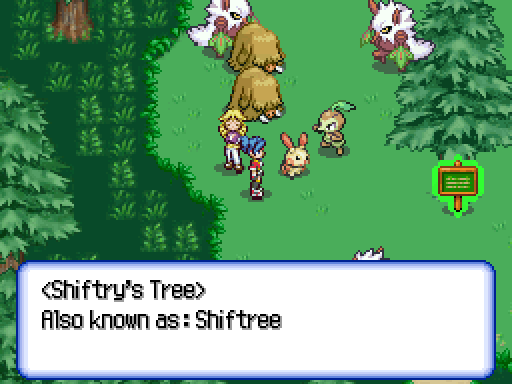
\includegraphics[width=.3\textwidth]{shiftree}} 


We will show the following equivalences:

\begin{itemize}
    \item \ref{eq:ex_otree_n} corresponds to \ref{eq:expandedDyck_n}
    \item \ref{eq:ex_otree_k1_1} corresponds to \ref{eq:expandedDyck_k1_1}
    \item \ref{eq:ex_otree_k1_0} corresponds to \ref{eq:expandedDyck_k1_0}
    \item \ref{eq:ex_otree_k} corresponds to \ref{eq:expandedDyck_k}
\end{itemize}

To accomplish this, we will first prove a few auxillary lemmas to be used to show equivalency between cases. 

Let $D=\dyck{T}$, $s$ be the number of consecutive ones to start D, and $z$ be the number of consecutive zeroes starting at $d_{s+1}$.  Note that $z=(k-s-1)$; $d_{k}=1$
% \begin{itemize}
\begin{lemma} \label{le:final_case_equivalence}

    $D$ has no 01 substring $\iff$ $\leftdown{T}=T$
\end{lemma}
\begin{proof}


    If $D$ has no $01$ substring, $D=1^n0^n$, and T is $n+1$ nodes where $t_0$ is the root and each $t_i$ for $1\le i \le n$ is a child of $t_{i-1}$  In this case, $T$ is a single path of $n+1$ nodes, and the left-down path of T is the entire tree.
\end{proof}
\begin{lemma} \label{le:no_children_equivalence}
    $D_{k+1} = 0 \iff O$ has no children
\end{lemma}
\begin{proof}

    This follows logically from the bijection between Dyck words and ordered trees.  $D_k$ corresponds to O.  If $D_{k+1}=0$, an ``upward" step is taken after O and consequently the next node after O cannot be a child of O.  Since the ones in $D$ give the nodes of T in preorder, O must have no children.

    Informally, once you go ``up" from O, the bijection between Dyck words and ordered trees gives no way to go ``back down" to give O an additional child.
\end{proof}
\begin{lemma} \label{le:tight_case_equivalence}
    $P=root \iff s=z=\frac{k-1}{2}$.
\end{lemma}
\begin{proof}

    First, note that $P=root$ simply means that O is a child of the root.  O is a child of the root $\iff \depth{O}=1$.  Additionally, note that $s+z=k-1$

    As shown in remark \ref{re:o_depth_formula}, $\depth{O}=s-z+1$. Therefore, $P=root \iff s=z=\frac{k-1}{2}$
    i.e. the first $k-1$ symbols of D are $\frac{k-1}{2}$ ones followed by $\frac{k-1}{2}$ zeroes. 

    % This equivalence can can be rewriten as follows: 

    % $s=k-s-1$

    % $2s=k-1$

    % $s=\frac{k-1}{2}$



\end{proof}
% \begin{enumerate}
\begin{lemma}
    \ref{eq:ex_otree_n} corresponds to \ref{eq:expandedDyck_n}
\end{lemma}
\begin{proof}

    Let $D=\dyck{T}$

    Per lemma \ref{le:final_case_equivalence} $D$ has no 01 substring $\iff$ $\leftdown{T}=T$.  

    Thus, $\nextTree{T}$ executes case \ref{eq:ex_otree_n} if and only if $\coolCat{D}$ executes case  \ref{eq:expandedDyck_n}

    Note that since $D$ has no $01$ substring, $D=1^n0^n$. 

    Additionally, since $\leftdown{T}=T$, T can be specified as follows.

    $T=$
    \begin{center}
	\begin{tabular}{ |c|c|c|c|c|c|c|c|c|c|c| } 
	    \hline

	    $node$ & $t_0$ & $t_1$  & $t_2$ & $\dots$ & $t_{n-1}$&$F=t_s=t_n$  \\
	    \hline
	    $depth$ & $0$ & $1$ & $2$ & $\dots$ & $n-1$ & $n$ \\
	    \hline
	    $Dyck$ &  &  \multicolumn{5}{|c|}{$1^n0^n$} \\
	    \hline
	\end{tabular}
    \end{center}

    The third row of this table illustrates the construction of $\dyck{T}$ via the process specified in remark \ref{re:construct_dyck}.

    Shifting $F$ to be the first child of the root changes $\depth{F}$ to 1 and does not affect the depth of any other nodes.  Thus, if $T'=\nextTree{T}$, 


    $T=$
    \begin{center}
	\begin{tabular}{ |c|c|c|c|c|c|c|c|c|c|c| } 
	    \hline

	    $node$ & $t_0$ & $F=t_s=t_n$ & $t_1$  & $t_2$ & $\dots$ & $t_{n-1}$  \\
	    \hline
	    $depth$ & $0$ & $1$ & $1$ & $2$ & $\dots$ & $n-1$ \\
	    \hline
	    $Dyck$ &  &  1 &  \multicolumn{4}{|c|}{$01^{n-1}0^{n-1}$} \\
	    \hline
	\end{tabular}
    \end{center}

    Recall that $\coolCat{D}=\preshift{D}{2n}$ if D has no 01 substring. $D_{2n}=0$, and therefore 

    $\coolCat{D}=101^{n-1}0^{n-1}$
     
     Note that this is exactly the Dyck word constructed from $T'$.  Therefore, if D has no 01 substring or $\leftdown{T}=T$, 

     $\otree{\coolCat{D}}=\nextTree{T}$

\end{proof}
\begin{lemma}
    \ref{eq:ex_otree_k1_0} corresponds to \ref{eq:expandedDyck_k1_0}
\end{lemma}
\begin{proof}
    Let $D=\dyck{T}$

    % \begin{itemize}
    Per lemma \ref{le:tight_case_equivalence} $P=root \iff D$ starts with exactly $\frac{k-1}{2}$ ones.  

    It was also previously shown that $D_{k+1}=0 \iff O$ has no children.  
    Thus, $\nextTree{T}$ executes case \ref{eq:otree_zeroshift} 
    if and only if $\coolCat{D}$ executes case   \ref{eq:expandedDyck_k1_0}

    \bigskip

    We now show that the execution of \ref{eq:otree_zeroshift} is equivalent to the execution of \ref{eq:expandedDyck_k1_0} given case a.
    Given $\dyck{T}=D=1^s0^{z}10d_{k+2}d_{k+3}...d_{2n}$, we aim to show that 

    $\dyck{\nextTree{T}}=\coolCat{\dyck{T}}$
    \bigskip

    Note that in this case $\nextTree{T}$ can be obtained by performing $\poppush{P}{G};\poppush{P}{root}$. 

	    Let $T'=\poppush[T]{P}{G}$; $T''=\poppush[T']{P}{root}$

    Note that $\nextTree{T}=T''$

    Since $P \ne root$, we know that G, the parent of P, exists. 
    Thus, we can assume that $G,P,L \in \leftdown{T}$.  T can therefore be specified as follows: 



    % this should be a little lemma
    % $T'$ shifts T so that L becomes the first child of G.  Note that L must have exactly 1 child: otherwise L's second child would be traversed earlier in a preorder traversal than O.  The same logic holds for each subtree of L: Each of L's non-leaf descendents must have exactly one child, as otherwise O would not be the first node in a preorder traversal of T not in $\leftdown{T}$.

    \bigskip
    \bigskip

    $T=$
    \begin{center}
	\begin{tabular}{ |c|c|c|c|c|c|c|c|c|c|c| } 
	    \hline

	    $node$ & $t_0$ & $t_1$ & $\dots$ & $G=t_{s-z-1}$ & $P=t_{s-z}$ & $L=t_{s-z+1}$ & $\dots$ & $F=t_s$ & $O=t_{s+1}$ & $\dots$ \\
	    \hline
	    $depth$ & $0$ & $1$ & $\dots$ & $(s-z-1)$ & $(s-z)$ & $(s-z+1)$ & $\dots$ & $s$  & $(s-z+1)$ & $\dots$\\
	    \hline
	    $Dyck$ &  &  \multicolumn{7}{|c|}{$1^s$} &  $0^{z}1$   & $0\dots$\\
	    \hline
	\end{tabular}
    \end{center}
    % Note that $|\leftdown{T'}|=s+1$; as it is nodes $t_0$ through $F$

    Furthermore, recall that L (and all other non-leaf nodes $\in \leftdown{T}$ must have exactly one child.  Therefore, every node below L in $\leftdown{T}$ has its depth reduced by one; no other nodes have their depth affected by this shift. Therefore, T' can be written as follows:

    \bigskip


    $T'=$
    \begin{center}
	\begin{tabular}{ |c|c|c|c|c|c|c|c|c|c|c| } 
	    \hline

	    $node$ & $t_0$ & $t_1$ & $\dots$ & $G=t_{s-z-1}$ & $L=t_{s-z+1}$ & $\dots$ & $F=t_s$ & $P=t_{s-z}$ & $O=t_{s+1}$ & $\dots$ \\
	    \hline
	    $depth$ & $0$ & $1$ & $\dots$ & $(s-z-1)$ & $(s-z)$ & $\dots$ & $s-1$ & $(s-z)$  & $(s-z+1)$ & $\dots$\\
	    \hline
	    $Dyck$ &  &  \multicolumn{6}{|c|}{$1^{s-1}$} &  $0^{z}1$   & $1$ & $0\dots$\\
	    \hline
	\end{tabular}
    \end{center}

    Since L is now G's first child, P changes from being G's first child to G's second child.  P is therefore removed from the left-down path of $T'$, thereby making P the first node in a preorder traversal of $T'$ that is not in the left-down path of $T'$.  
    Therefore, $|\leftdown{T'}|=s$; $O'=P$. % TODO: check this

    % Note in the case where $z=1$, $L=F=t_s$; i.e. L is the leaf of the left-down path of T.

    Recovering a Dyck word from $T'$, we obtain 

    D'=$1^{s-1}0^z110d_{k+2}d_{k+3},\dots,d_{2n}$


    Next, we use $\poppush[T']{P}{root}$
 to obtain $T'' = \nextTree{T}$

    $\poppush[T']{P}{root}$
 shifts O to become the first child of the root. Note that we know that O has no children. Consequently, no nodes other than O have their depth affected by this shift. Thus, 

    \bigskip
    \bigskip


    % TODO: tm+2 dots, here and other tables
    $T''=$
    \begin{center}
	\begin{tabular}{ |c|c|c|c|c|c|c|c|c|c|c|c| } 
	    \hline

	    $node$ & $t_0$ & $O=t_{s+1}$ & $t_1$ & $t_2$ & $\dots$ & $G=t_{s-z-1}$ & $L=t_{s-z+1}$ & $\dots$ & $F=t_s$ & $P=t_{s-z}$ & $\dots$ \\
	    \hline
	    $depth$ & $0$ & $1$ & $1$ & $2$ &$\dots$ & $(s-z-1)$ & $(s-z)$ & $\dots$ & $s-1$ & $(s-z)$   & $\dots$\\
	    \hline
	    $Dyck$ &  & $1$ &  \multicolumn{7}{|c|}{$01^{s-1}$} &  $0^{z}1$   & $\dots$\\
	    \hline
	\end{tabular}
    \end{center}


    % Next, recovering a Dyck word from $$
    \bigskip
    \bigskip

    % TODO: refine



    Therefore, since $T''=\nextTree{T}$, $\dyck{\nextTree{T}}=101^{s-1}0^z1\dots$

    Since $\dyck{T}=D=1^s0^{z}10\dots$
    $\ref{eq:expandedDyck_k1_1}$ gives that

    $\coolCat{\dyck{T}}=101^{s-1}0^z1\dots$

    Therefore, we have shown that $\dyck{\nextTree{T}}=\coolCat{\dyck{T}}=101^{s-1}0^z1\dots$
    % \end{itemize}

\end{proof}
\begin{lemma}
    \ref{eq:ex_otree_k1_1} corresponds to \ref{eq:expandedDyck_k1_1}
\end{lemma}
\begin{proof}

    Per \ref{le:no_children_equivalence}, as $O$ has at least 1 child $\iff D_{k+1}=1$.
    % Note that the conditions for \ref{eq:ex_otree_k1_1} and \ref{eq:expandedDyck_k1_1} are equivalent, as $O$ has at least 1 child $\iff D_{k+1}=1$.

    Thus, $\nextTree{T}$ will execute case \ref{eq:ex_otree_k1_1} if and only if $\coolCat{D}$ executes case \ref{eq:expandedDyck_k1_1}

    Therefore, we aim to show that, given O has at least one child and $D_{k+1}=1$,

    $\preshift{\dyck{T}}{k+1}=\dyck{\poppush[T]{P}{O}}$

    Since $D_{k+1}=1$, we can rewrite D as.
    $D=1^s0^z11$


    \noindent $T=$
    \begin{center}
	\begin{tabular}{ |c|c|c|c|c|c|c|c|c|c|c|c| } 
	    \hline

	    $node$ & $t_0$ & $t_1$ & $\dots$ & $G=t_{s-z-1}$ & $P=t_{s-z}$ & $L=t_{s-z+1}$ & $\dots$ & $F=t_s$ & $O=t_{s+1}$ & $t_{s+2}\dots$ \\
	    \hline
	    $depth$ & $0$ & $1$ & $\dots$ & $(s-z-1)$ & $(s-z)$ & $(s-z+1)$ & $\dots$ & $s$  & $(s-z+1)$ & $s-z+2 \dots$\\
	    \hline
	    $Dyck$ &  &  \multicolumn{7}{|c|}{$1^s$} &  $0^{z}1$   & $1\dots$\\
	    \hline
	\end{tabular}
    \end{center}

    $\poppush[T]{P}{O}$
    shifts L to be O's first child:

    Nodes $L=t_{s-z+1}$ through $F=t_s$ will now come after O in preorder traversal.  Additionally, $\leftdown{T}$ will now go through O; every node in $\path{T}{L}{F}$ will have its depth increased by one.  

    Therefore, $T'=\nextTree{T}$ can be specified as follows: 

    \noindent $T'=$
    \begin{center}
	\begin{tabular}{ |c|c|c|c|c|c|c|c|c|c|c|c| } 
	    \hline

	    $node$ & $t_0$ & $t_1$ & $\dots$ & $G=t_{s-z-1}$ & $P=t_{s-z}$ & $O=t_{s+1}$ & $L=t_{s-z+1}$ & $\dots$ & $F=t_s$  & $t_{s+2}\dots$ \\
	    \hline
	    $depth$ & $0$ & $1$ & $\dots$ & $(s-z-1)$ & $(s-z)$ & $(s-z+1)$ & $(s-z+2)$ & $\dots$ & $s+1$  & $s-z+2 \dots$\\
	    \hline
	    $Dyck$ &  &  \multicolumn{8}{|c|}{$1^{s+1}$}  & $0^{z}1\dots$\\
	    \hline
	\end{tabular}
    \end{center}

    Note that $z \ge 1$, so $z$ zeroes occur between the one corresponding to $t_{s}$ and the one corresponding to $t_{s+2}$.


    Next, recall that $D=\dyck{T}=D=1^s0^z11\dots$ and that $k=s+z+1$

    Therefore, $\coolCat{D}=\preshift{D}{k+1}=1^{s+1}0^z1\dots$, which is the same as the Dyck word resulting from translating $T'=\nextTree{T}$ to the Dyck word $1^{s+1}0^z1\dots$

\end{proof}
\begin{lemma}
    \ref{eq:ex_otree_k} corresponds to \ref{eq:expandedDyck_k}
\end{lemma}
\begin{proof}

    $T \ne \leftdown{T} \iff D$ has a 01 substring.

    $D_{k+1}=1 \iff O$ has at least one child.

    $D_{k+1}=0$ and $s=\frac{k-1}{2} \iff O$ has no children and O is a child of the root.

    O has no children and P=root. Therefore $s=z$, $k=2s+1$

    We can thus rewrite $D=\dyck{T}=1^s0^s101\dots$

    Furthermore, since $s=z$, O has depth 1. 

    Therefore, we can write T as 
    \noindent $T=$
    \begin{center}
	\begin{tabular}{ |c|c|c|c|c|c|c|c|c|c|c|c| } 
	    \hline

	    $node$ & $P=t_0$ & $L=t_1$ & $\dots$ & $F=t_s$ & $O=t_{s+1}$ & $t_{s+2}\dots$ \\
	    \hline
	    $depth$ & $0$ & $1$ & $\dots$ & $s$ & $1$ & $1$ \\
	    \hline
	    $Dyck$ &  &  \multicolumn{3}{|c|}{$1^s$} &  $0^{s}1$   & $01\dots$\\
	    \hline
	\end{tabular}
    \end{center}


    $\poppush[T]{P}{O}$
    shifts L to be O's first child:

    Therefore, nodes $L=t_{1}$ through $F=t_s$ will now come after O in preorder traversal.  Additionally, $\leftdown{T}$ will now go through O; every node in $\path{T}{L}{F}$ will have its depth increased by one.  

    Therefore, $T'=\nextTree{T}$ can be specified as follows: 

    \noindent $T'=$
    \begin{center}
	\begin{tabular}{ |c|c|c|c|c|c|c|c|c|c|c|c| } 
	    \hline

	    $node$ & $P=t_0$ & $O=t_{s+1}$& $L=t_1$ & $\dots$ & $F=t_s$  & $t_{s+2}\dots$ \\
	    \hline
	    $depth$ & $0$ & $1$ & $2$ & $\dots$ & $s+1$ & $1$  \\
	    \hline
	    $Dyck$ &  &  \multicolumn{4}{|c|}{$1^{s+1}$} &  $0^{s+1}1\dots$   \\
	    \hline
	\end{tabular}
    \end{center}

Since $D=\dyck{T}=1^s0^s101\dots$, $\coolCat{D}=1^{s+1}0^{s+1}1\dots$ as per case $\ref{eq:ex_otree_k}$.  This is identical to the Dyck word constructed from $T'=\nextTree{T}$.  Therefore, cases \ref{eq:ex_otree_k} and \ref{eq:expandedDyck_k} are equivalent.

\end{proof}

Since these 4 cases cover all cases for the two successor rules, we have shown that $\nextTree{T}=\otree{\coolCat{\dyck{T}}}$ in all cases. 
\end{proof}


This chapter provides two loopless implementations of the Gray code given in Chapter \ref{chap:otree-graycode}.  
Section \ref{sec:relationship-loopless} discusses this chapter's algorithm in the context of other related results.  Section \ref{sec:looples-approach} discusses the common approach used in both loopless implementations.  Section \ref{sec:otree-link} provides an implementation using a linked-list like structure for storing children.  Section \ref{sec:otree-arr} provides an implementation using an array to store children.  


\section{Relationship to Previous Results}\label{sec:relationship-loopless}
The algorithms in Sections \ref{sec:otree-link} and \ref{sec:otree-arr} both generate ordered trees \emph{looplessly}, meaning that each tree is generated in worst-case constant time.  This is faster than other algorithms for generating ordered trees which take constant amortized time \cite{parque2021efficient} \cite{er1985lexotrees} \cite{zaks1980lexotrees} \cite{skarbek1988pointerotrees}. 

%Parque and Miyashita present a constant amortized time algorithm for generating ordererd trees, claiming that it operates ``with utmost efficiency'' \cite{parque2021efficient}.  Our algorithm operates in worst-case constant time per tree, which is faster. To borrow Parque and Miyashita's terminology, perhaps we should say that our algorithm operates with \emph{utmoster} efficiency. 

Taken in conjunction with Ruskey and Williams's algorithms for Dyck words and binary trees, this algorithm completes a trio of loopless cool-lex algorithms for enumerating the three foremost Catalan structures.  
Additionally, like the cool-lex algorithm for binary trees, this algorithm generates ordered trees stored as pointer structures.  This contrasts from other efficient Gray codes for enumerating ordered trees, which use either bit-strings or integer sequences to represent ordered trees \cite{parque2021efficient} \cite{zaks1980lexotrees} \cite{er1985lexotrees} as representations of ordered trees.  Skarbek's 1988 paper \emph{Generating Ordered Trees} gives a constant amortized time algorithm for generating ordered trees stored as pointer structures and is therefore a notable exception to this \cite{skarbek1988pointerotrees}.  Generating ordered trees via a pointer structure facilitates the practical %TODO: word?
use of the trees generated by this algorithm, as a translation step between an alternative representation and a tree structure is not necessary to traverse the tree .

Korsh and Lafollette \cite{korsh2000multiset} gave a loopless algorithm for generating ordered trees with a fixed branching sequence.  In other words, they generated subsets of ordered trees with a fixed number of nodes for which a listing of the number of children at each node form the same multiset.  Their algorithm used a string-based representation rather than a link-based representation, and thus answered a challenging open problem posed by van Baronaigen \cite{van1991loopless}.   They also stated, in one sentence, that their results could be adapted to a link-based representation.  By `layering' the output of that proposed algorithm, it may be possible to create a loopless link-based algorithm for generating all ordered trees with $n$ nodes.  It is also important to note that the results in \cite{korsh2000multiset} are not simple: the provided C code includes over one hundred instances of the \verb$if$ and \verb$else$ keywords.

\section{Loopless Approach}\label{sec:looples-approach}
The algorithms for both the linked-list and array representations of ordered trees take the following approach.  They begin by creating an initial tree $\tree{T}_1$ with $n+1$ nodes such that $\dyck{\tree{T}_1}=101^{n-1}0^{n-1}$.  This tree can be generated by creating a path with $n+1$ nodes and executing $\pull{root}{P}$ where $P$ is the parent of the path's leaf. Both algorithms then repeatedly apply the successor rule from equation \eqref{eq:otreeRule}.  The algorithms keep track of $O$ using the observation that if $O$ has at least one child before shifting, the new first branching is between $O$ and $O$'s second child after shifting.  If $O$ has no children before shifting, the new first branching is between $P$ and $P$'s second child after shifting. Figures \ref{fig:otreeCode} and \ref{fig:aotreeCode} provide pseudocode and a C implementation for this algorithm using each tree representation.  Full source code for both of these algorithms in C is available here \cite{lapeythesisrepo}.


\section{Storing Children in a Linked List}\label{sec:otree-link}

The implementation in this section uses a linked structure to store a node's children, where an ordered tree node stores pointers to its first (leftmost) child and its right sibling.  Therefore, to access a node's 3rd child, one would use \verb+node->first->right->right+.
This has the advantages of space efficiency and $O(1)$ time for appending and prepending to a node's list of children, but the disadvantage of requiring $O(k)$ time to access a node's $k\thh$ child. 

Figure \ref{fig:otreestarter-link} provides the C struct definition for this ordered tree definition as well as an implementation of $\pull{A}{B}$ and a helper function for accessing a node's $k\thh$ child. 

\begin{figure}
    % \begin{subfigure}[t]{.5 \textwidth}
	\begin{center}

	    \begin{Verbatim}
typedef struct node {
  struct node* parent;
  struct node* first;
  struct node* right;
} node;

void pull(node *A, node *B){ 
  // A pulls B's first child
  node *pulled = B->first;
  B->first = pulled->right;
  pulled->right = A->first;
  A->first = pulled;
  pulled->parent = A;
}

node* kthchild(node* parent, int k){
  node* curr=parent->first;
  for(int i = 1; i < k; i++){
    curr=curr->right;
  }
  return curr;
}
\end{Verbatim}

    \cprotect\caption{Struct definitions and implementations for $\pull{A}{B}$ and accessing a $k\thh$ child for a link-based ordered tree structure.}
\label{fig:otreestarter-link}
	\end{center}
\end{figure}

    The algorithm in Figure \ref{fig:otreeCode} uses a while loop with two if statements per successor to evaulate the cases in \eqref{eq:otreeRule}.  The while loop evaluates if there is a first branching: if \verb+NULL+ is assigned to $O$, then there is no first branching, and the order is complete.  The first if statement evaluates whether $O$ has at least 1 child: $O$'s first child is not \verb+NULL+ if and only if O has at least 1 child. The second if statement evaluates whether $P$ is the root of the tree.  The algorithm executes $\pull{O}{P}$ if $O$ has at least child or $P$ is the root of the tree.  Otherwise, it executes $\pull{G}{P}$ and $\pull{root}{P}$.  The algorithm keeps track of $O$ via the observation that if $O$ has at least one child before shifting, the new first branching is between $O$ and $O$'s second child after shifting and if $O$ has no children before shifting, the new first branching is between $P$ and $P$'s second child after shifting. This translates to assigning \verb+o = o->first->right+ if O has at least 1 child and \verb+o = o->right+ otherwise.

    This implementation is very clearly loopless, as $\pull{A}{B}$ is a constant time operation and only two if statements and the condition of the while loop are evaluated per successor.


\begin{figure}[H]
    \centering
    \begin{subfigure}[t]{.49 \textwidth}
	\begin{center}
	    \begin{algorithm}[H] % What does the H do? it makes it work.
	    \begin{algorithmic}
    \Function{cool-ordered-trees}{$t$}
        % \vspace{0.75em}
        \LineComment{Generate initial tree} % TODO
	\State $O\gets root.first$
	\State \visit{root}
        \While{$O \ne NULL$}
	    \State $P \gets O.parent$
	    \If{$O.first \ne NULL$}
		\State $\pull{O}{P}$
		\State $O \gets O.first.right$
	    \Else
		\If{$P == root$}
		\State $\pull{O}{P}$
		\Else
		\State $\pull{O}{P}$
		\State $\pull{root}{P}$
		\EndIf
		\State $O \gets O.right$
	    \EndIf
	\State \visit{root}
        \EndWhile
    \EndFunction
	    \end{algorithmic}
    \caption*{Generate all ordered trees with $t+1$ nodes}
	\end{algorithm}
	\end{center}
	% \caption{Pseudoc}
	\label{fig:}
    \end{subfigure}
    \begin{subfigure}[t]{.5 \textwidth}
	\begin{center}
	    \vspace{.9em} % fun alignment
	    % \vspace{2.1em} % fun alignment
\begin{Verbatim}[commandchars=\\\[\]]

void coolOtree(int n) {
  node* root = get_initial_tree(n);
  node* o=root->first->right;
  visit(root);
  while (o) {
    p=o->parent;
    if (o->first) {
      pull(o,p);
      o = o->first->right;
    } else {
      if (p == root) {
        pull(o,p);
      } else {
        pull(p->parent,p);
        pull(root,p);
      }
      o = o->right;
    }
    visit(root);
  }
}

\end{Verbatim}
	\end{center}
	% \caption{ $C$ implementation of coolOtree} 
	\label{fig:}
    \end{subfigure}
    % TODO: change bit colors
    \cprotect\caption{Pseudocode and C implementation for linked-list tree representation.}
    \label{fig:otreeCode}
\end{figure}

\section{Storing Children in an Array}\label{sec:otree-arr}
The second implementation uses an array-like approach to storing children.  This has the advantage of $O(1)$ access time for all children but the disadvantage of either requiring $O(n)$ space for each node or the additional cost of resizing arrays.  Each node also stores a counter for its number of children and a number keeping track of the maximum amount of children it can store (before requiring reallocation).  This implementation stores the list of children ``backwards,'' so that the array can be operated on like a stack.  In particular, this allows for pushing and popping first children without shifting the whole array. Each \verb+node->children[0]+ is set to and kept as \verb+NULL+ for a null-termination like effect that is useful in the algorithm. Therefore, to access a node's $k\thh$ child, one would use \verb_node->children[(node->nch)-k+1]_.  The \verb+kthchild+ function simplifies accessing a node's $k\thh$ child and is used in our implementation.  Figure \ref{fig:otreestarter-arr} provides the C struct definition for this ordered tree definition as well as an implementation of $\pull{A}{B}$ and a \verb+kthchild+. 

    Like the linked-list implementation in Figure \ref{fig:otreeCode}, the array based implementation in Figure \ref{fig:aotreeCode} uses a while loop with two if statements per successor to evaulate the cases in \eqref{eq:otreeRule}.  The logical structure of the while loop and if statements is identical to that of \ref{fig:aotreeCode}: the while loop terminates when there is no first branching, the first if statement evaluates whether $O$ has at least 1 child, and the second if statement evaluates whether $P$ is the root of the tree.  The algorithms in \ref{fig:otreeCode} and \ref{fig:aotreeCode} are almost identical apart from the structure they use and the implementation differences between between \verb+pull+ and \verb+apull+.

    \begin{figure}
	\begin{center}

	    \begin{Verbatim}
typedef struct arraynode {
    int nch; 
    int maxch;
    struct arraynode* parent;
    struct arraynode** children;
} anode;

void apull(anode* A, anode* B){ 
    //A pulls B's first child
    anode* pulled = B->children[B->nch--];
    A->children[++(A->nch)]=pulled;
    pulled->parent=A;
}

anode* kthchild(anode* parent, int k){
  return parent->children[parent->nch-k+1];
}
	    \end{Verbatim}
	\end{center}
    % \end{subfigure}

    % TODO: change bit colors
    \cprotect\caption{Struct definitions and implementations for $\pull{A}{B}$ and accessing a $k\thh$ child for an array-based ordered tree structure.}
    \label{fig:otreestarter-arr}
\end{figure}

\begin{figure}
    \centering
    \begin{subfigure}[t]{.49 \textwidth}
	\begin{center}
	    \begin{algorithm}[H] % What does the H do? it makes it work.
	    \begin{algorithmic}
    \Function{cool-ordered-trees}{$n$}
        % \vspace{0.75em}
        \LineComment{Generate initial tree} % TODO
		\State $O\gets \kthchild{root}{2}$
	\State \visit{root}
        \While{$O \ne NULL$}
	    \State $P \gets O.parent$
	    \If{$O.nch > 0$}
		\State $\pull{O}{P}$
		\State $O \gets \kthchild{O}{2}$
	    \Else
		\If{$P == root$}
		\State $\pull{O}{P}$
		\Else
		\State $\pull{P.parent,P}$
		\State $\pull{root,P}$
		\EndIf
		\State $O \gets \kthchild{O.parent}{2}$
	    \EndIf
	\State \visit{root}
        \EndWhile
    \EndFunction
	    \end{algorithmic}
    \caption*{Generate all ordered trees with $n+1$ nodes}
	\end{algorithm}
	\end{center}
	% \caption{Pseudoc}
	\label{fig:}
    \end{subfigure}
    \begin{subfigure}[t]{.5 \textwidth}
	\begin{center}
	    \vspace{.9em} % fun alignment
	    % \vspace{2.1em} % fun alignment
\begin{Verbatim}[]

void coolAOtree(int t, void (*visit)(anode*)){
  anode* root = get_initial_atree(t);
  anode *p, *o=kthchild(root,2);
  visit(root);
  while(o){
    p = o->parent;
    if(o->nch){
      apull(o,p);
      o=kthchild(o,2);
    }else{
      if(p == root){
	apull(o,p);
      }else{
	apull(p->parent,p);
	apull(root,p);
      }
      o=kthchild(o->parent,2);
    }
    visit(root);
  }
}

\end{Verbatim}
	\end{center}
	% \caption{ $C$ implementation of coolOtree} 
	\label{fig:}
    \end{subfigure}
    % TODO: change bit colors
    \cprotect\caption{Pseudocode and C implementation for array-based tree representation.}
    \label{fig:aotreeCode}
\end{figure}



\chapter{Lattice Paths: Lukasiewicz, Motzkin, Schroder}
TODO: this needs to be organized

Motzkin, Schröder, and Łukasiewicz paths provide generalizations of Dyck words.  

Recall the interpretation of Dyck words as paths in the Cartesian plane from Section \ref{sec:Dycks}.

Motzkin paths allow for (1,0) horizontal steps in addition to (1,1) and (1,-1) steps. Schröder paths are identical to Motzkin paths except they allow for $(2,0)$ horizontal steps instead of $(1,0)$.  Łukasiewicz paths allow (1,-1) steps, (1,0) steps and any (1,k) step where k is a positive integer.  All three languages retain the requirement that the path start at the origin, end on the x axis, and never step below the x axis. 

These paths can be encoded in a number of different ways.  In a \emph{-1-based encoding}, each $(1,i)$ step is encoded as i, and every prefix must have a nonnegative sum.  In a \emph{0-based encoding}, each $(1,i)$ step is encoded as $i+1$, and the sum of every prefix must be as large as its length. We primarily use the 0-based encoding. See Fig. \ref{fig:paths}  for examples of these paths using the 0-based encoding.

We refer to Motzkin, Schröder, and Lukasiewicz paths ending at $(n,0)$ as paths of \emph{order n}.  This contrasts slightly with the classification of Dyck words of order n, which terminate at $(2n,0)$

In the context of fixed-content generation, Motzkin and Schröder paths are identical:  Both will have northeast steps encoded as twos, horizontal steps encoded as ones, and southeast steps encoded as zeroes.  However, their Cartesian plane representations will differ in the length of horizontal steps. Notably, Łukasiewicz are a generalization of Motzkin paths, as any Motzkin path is also a Lukasiewicz path.

\begin{figure}[]
	\centering
	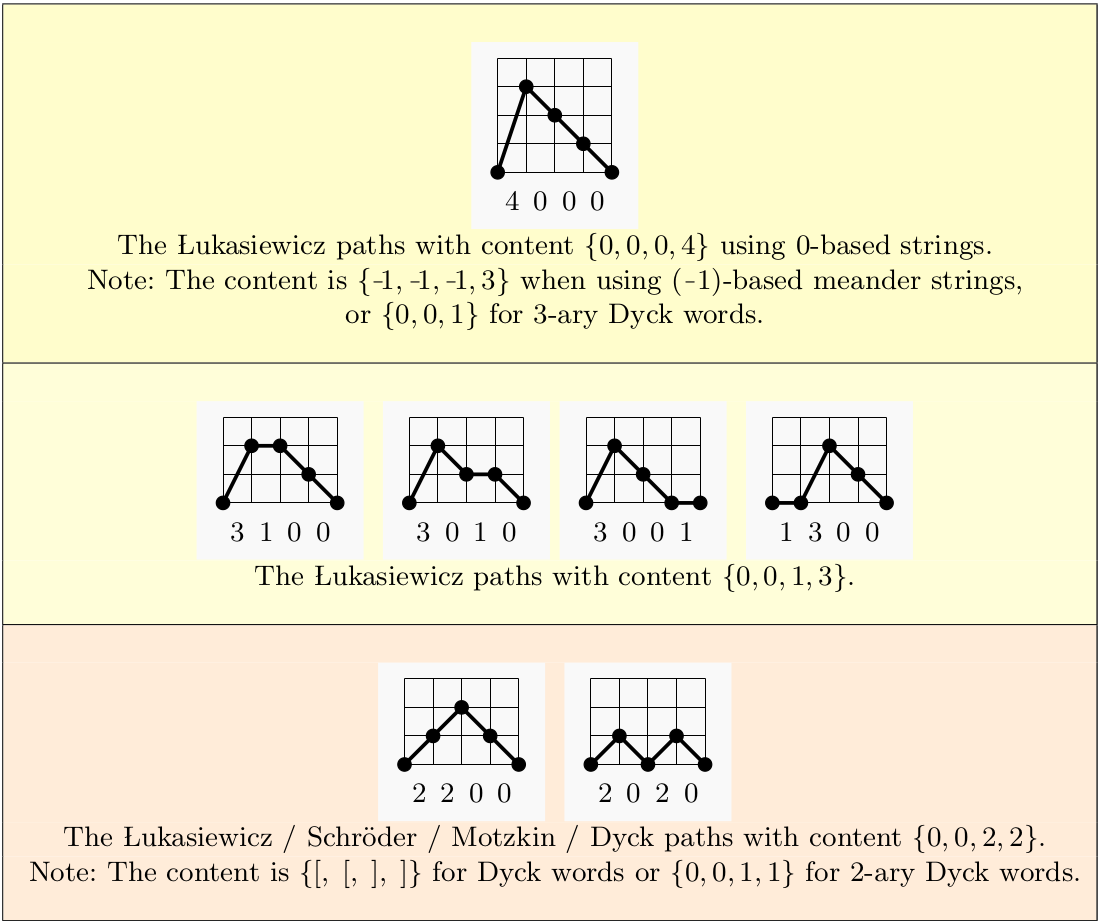
\includegraphics[width = .95 \textwidth]{paths.png}
	\caption{}
	\label{fig:paths}
\end{figure}


The number of Dyck words with n zeroes and n ones are counted by the $n\thh$ Catalan number.  Similarly, the number of Motzkin and Schröder paths of order $n$ are counted by the $n\thh$ Motzkin and big Schröder number respectively. The number of Lukasiewicz paths of order $n$ are counted by the n
Motzkin, Schröder, and Lukasiewicz paths bear a number of interesting bijective correspondences with other combinatorial objects. Richard Stanely's \emph{Catalan Objects} outlines hundreds of interesting examples.  

Lukasiewicz paths  of order $n$ bear a particularly nice correspondence to rooted ordered trees with $n+1$ nodes. See Fig. \ref{trees} for an illustration of this.

\begin{figure}[]
	\centering
	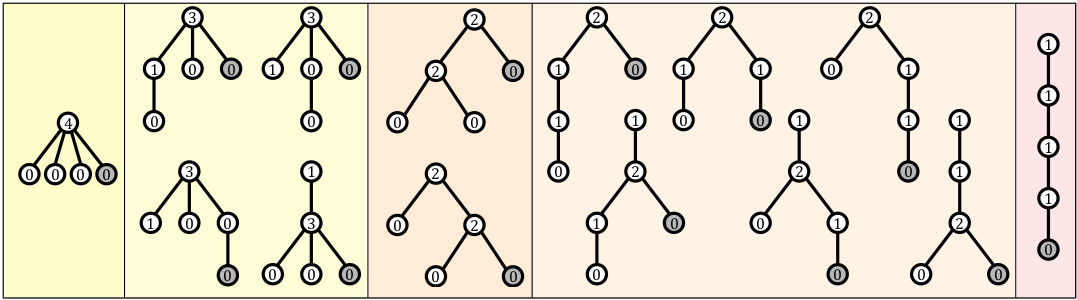
\includegraphics[width = .95 \textwidth]{trees.png}
	\caption{The $\mathcal{C}_4$=14 Lukasiewicz paths of order $n=4$ are in bijective correspondence with the 14 rooted ordered trees with $n+1=5$ nodes.  Given a tree, the corresponding word is obtained by recording the number of children of each node in preorder traversal; the zero from the rightmost leaf is omitted.  For example, the two trees in the middle section correspond to 2200 (top) and 2020 (bottom) respectively.}
	\label{trees}
\end{figure}

% TODO: bijections, mirror chapter 2



In this chapter, we give a Gray code for generating Łukasiewicz words with fixed content using left-shifts. Section \ref{sec:lukasuc} will give the successor rule for the Gray code; Section \ref{sec:lukaproof} will prove its correctness.
\section{Successor Rule}\label{sec:lukasuc}

In this section, we provide a successor rule that applies a left-shift to a Łukasiewicz word.  The rule is given below in \eqref{eq:luka}.
Let $S$ be a multiset whose sum is equal to its length.  Let $\mathcal{L}(S)$ denote the set of valid Łukasiewicz words with content equal to S. Let $\alpha \in \mathcal{L}(S)$.  


Recall the definition of a left-shift from equation \eqref{eq:leftdef}: $\lshiftindex[\alpha]{i}{j}$ shifts the $j\thh$ symbol in $\alpha$ into the $i\thh$ position. 
% As in the cool-lex successor rule for multiset permutations in \ref{sec:coolPerms}, we let $x$ be the smallest value for which $\alpha_x<\alpha_{x-1}$.  
We also let $\rho=\alpha_1\cdot\alpha_2\cdots\alpha_{m}$ be the non-increasing prefix of $\alpha$, i.e. the longest prefix of $\alpha$ such that $\alpha_{i}\ge\alpha_{i-1}$ for all $i \le m$.  
%In addition to the left-shift function, we define the length of the \emph{non-increasing prefix} of a string $\alpha$ to be 
%the maximum value $m$ such that $\alpha_{i-1} \ge \alpha_{i}$ for all $2 \le i \le m$. We will let $\rho$ $\rho = a_1 \cdot a_2 \cdots a_m$.  The sum of the symbols in $\rho$ is $\sum \rho = a_1 + a_2 + \cdots + a_m$


\begin{subnumcases}{\luka{\alpha} = \label{eq:luka}} 
    \lshiftindex{n}{2} & if  $m=n$ \label{eq:prefix_n_2}\\
	\lshiftindex{m+1}{1} & if  $m=n-1$  or  $\alpha_{m} < \alpha_{m+2}$   or $(\alpha_{m+2} = 0 $ and $ \sum \rho = m) $ \label{eq:prefix_m1_1}\\
	\lshiftindex{m+2}{1} &  if $ \alpha_{m+2} \neq 0 $\label{eq:prefix_m2_1}\\
	\lshiftindex{m+2}{2} & otherwise  \label{eq:prefix_m2_2}
\end{subnumcases}

% \begin{subnumcases}{\luka{\alpha} = \label{eq:luka}} 
%     \lshiftindex{n}{2} & if  $\alpha$ is in descending order \label{eq:prefix_n_2}\\
% 	\lshiftindex{x}{1} & if  $x=n$  or  $\alpha_{x-1} < \alpha_{x+w}$   or \label{eq:prefix_m1_1}\\
% 	    & $(\alpha_{x+1} = 0 $ and $ \sum \rho = x-1) $\nonumber\\
% 	\lshiftindex{m+2}{1} &  if $ \alpha_{m+2} \neq 0 $\label{eq:prefix_m2_1}\\
% 	\lshiftindex{m+2}{2} & otherwise  \label{eq:prefix_m2_2}
% \end{subnumcases}

Figure \ref{fig:LukaTable} illustrates the successor rule on every string in $\Lukas{S}$ for $S = \{0,0,0,1,2,3\}$.
For example, consider the top row with $\alpha = a_1 \cdot a_2 \cdot a_3 \cdot a_4 \cdot a_5 \cdot a_6 = 302100$.
Here the non-increasing prefix is $a_1 \cdot a_2 = 30$, so $x = 1$, and the length of the string is $n = 6$.
Thus, $x \neq n$, so \eqref{eq:prefix_n_2} is not applied.
Now consider the conditions in \eqref{eq:prefix_m1_1}.
The second condition is $a_{m} < a_{m+2}$, which is $a_2 = 0 < 1 = a_4$ for $\alpha$.  
Since this is true, $\luka{\alpha} = \lshiftindex{m+1}{1}$ by \eqref{eq:prefix_m1_1}, which is $\lshiftindex{3}{1}$ for $\alpha$.
In other words, the rule left-shifts $a_3$ into position $1$.
Thus, the next string in the list is $a_3 \cdot a_1 \cdot a_2 \cdot a_4 \cdot a_5 \cdot a_6 = 230100$, as seen in the second row of Figure~\ref{fig:LukaTable}.


\begin{figure}
    \centering
    % This figure is temporarily omitted because it is slow
    \begin{tabularx}{0.9\textwidth}{>{\hsize=0.275\hsize}C >{\hsize=0.225\hsize}C >{\hsize=0.05\hsize}C >{\hsize=0.1\hsize}C >{\hsize=0.2\hsize}C  >{\hsize=0.2\hsize}r }
\thead{Łukasiewicz path} & \thead{Łukasiewicz word} & \thead{$m$} & \thead{\eqref{eq:luka}} & \thead{shift} & \thead{scut} \\ \hline 
\LukaTable[2]{3,0,2,1,0,0} & 302100 & 2 & \eqref{eq:prefix_m1_1} & $\lshiftindex{3}{1}$ & $100$ \\
\LukaTable[3]{2,3,0,1,0,0} & 230100 & 1 & \eqref{eq:prefix_m2_2} & $\lshiftindex{3}{2}$ & $100$ \\
\LukaTable[2]{2,0,3,1,0,0} & 203100 & 2 & \eqref{eq:prefix_m1_1} & $\lshiftindex{3}{1}$ & $100$ \\
\LukaTable[3]{3,2,0,1,0,0} & 320100 & 3 & \eqref{eq:prefix_m2_2} & $\lshiftindex{5}{2}$ & $100$ \\
\LukaTable[2]{3,0,2,0,1,0} & 302010 & 2 & \eqref{eq:prefix_m2_2} & $\lshiftindex{4}{2}$ & $10$ \\
\LukaTable[2]{3,0,0,2,1,0} & 300210 & 3 & \eqref{eq:prefix_m1_1} & $\lshiftindex{4}{1}$ & $10$ \\
\LukaTable[3]{2,3,0,0,1,0} & 230010 & 1 & \eqref{eq:prefix_m2_2} & $\lshiftindex{3}{2}$ & $10$ \\
\LukaTable[2]{2,0,3,0,1,0} & 203010 & 2 & \eqref{eq:prefix_m1_1} & $\lshiftindex{3}{1}$ & $10$ \\
\LukaTable[3]{3,2,0,0,1,0} & 320010 & 4 & \eqref{eq:prefix_m2_2} & $\lshiftindex{6}{2}$ & $10$ \\
\LukaTable[2]{3,0,2,0,0,1} & 302001 & 2 & \eqref{eq:prefix_m2_2} & $\lshiftindex{4}{2}$ & $1$ \\
\LukaTable[2]{3,0,0,2,0,1} & 300201 & 3 & \eqref{eq:prefix_m1_1} & $\lshiftindex{4}{1}$ & $1$ \\
\LukaTable[3]{2,3,0,0,0,1} & 230001 & 1 & \eqref{eq:prefix_m2_2} & $\lshiftindex{3}{2}$ & $1$ \\
\LukaTable[2]{2,0,3,0,0,1} & 203001 & 2 & \eqref{eq:prefix_m1_1} & $\lshiftindex{3}{1}$ & $1$ \\
\LukaTable[3]{3,2,0,0,0,1} & 320001 & 5 & \eqref{eq:prefix_m1_1} & $\lshiftindex{6}{1}$ & $1$ \\
\LukaTable[3]{1,3,2,0,0,0} & 132000 & 1 & \eqref{eq:prefix_m1_1} & $\lshiftindex{2}{1}$ & $2000$ \\
\LukaTable[3]{3,1,2,0,0,0} & 312000 & 2 & \eqref{eq:prefix_m2_2} & $\lshiftindex{4}{2}$ & $2000$ \\
\LukaTable[2]{3,0,1,2,0,0} & 301200 & 2 & \eqref{eq:prefix_m1_1} & $\lshiftindex{3}{1}$ & $200$ \\
\LukaTable[2]{1,3,0,2,0,0} & 130200 & 1 & \eqref{eq:prefix_m1_1} & $\lshiftindex{2}{1}$ & $200$ \\
\LukaTable[2]{3,1,0,2,0,0} & 310200 & 3 & \eqref{eq:prefix_m2_2} & $\lshiftindex{5}{2}$ & $200$ \\
\LukaTable[2]{3,0,1,0,2,0} & 301020 & 2 & \eqref{eq:prefix_m2_2} & $\lshiftindex{4}{2}$ & $20$ \\
\LukaTable[2]{3,0,0,1,2,0} & 300120 & 3 & \eqref{eq:prefix_m1_1} & $\lshiftindex{4}{1}$ & $20$ \\
\LukaTable[2]{1,3,0,0,2,0} & 130020 & 1 & \eqref{eq:prefix_m1_1} & $\lshiftindex{2}{1}$ & $20$ \\
\LukaTable[2]{3,1,0,0,2,0} & 310020 & 4 & \eqref{eq:prefix_m1_1} & $\lshiftindex{5}{1}$ & $20$ \\
\LukaTable[3]{2,3,1,0,0,0} & 231000 & 1 & \eqref{eq:prefix_m2_1} & $\lshiftindex{3}{1}$ & $31000$ \\
\LukaTable[3]{1,2,3,0,0,0} & 123000 & 1 & \eqref{eq:prefix_m1_1} & $\lshiftindex{2}{1}$ & $3000$ \\
\LukaTable[3]{2,1,3,0,0,0} & 213000 & 2 & \eqref{eq:prefix_m2_2} & $\lshiftindex{4}{2}$ & $3000$ \\
\LukaTable[2]{2,0,1,3,0,0} & 201300 & 2 & \eqref{eq:prefix_m1_1} & $\lshiftindex{3}{1}$ & $300$ \\
\LukaTable[2]{1,2,0,3,0,0} & 120300 & 1 & \eqref{eq:prefix_m1_1} & $\lshiftindex{2}{1}$ & $300$ \\
\LukaTable[2]{2,1,0,3,0,0} & 210300 & 3 & \eqref{eq:prefix_m1_1} & $\lshiftindex{4}{1}$ & $300$ \\
\LukaTable[3]{3,2,1,0,0,0} & 321000 & 6 & \eqref{eq:prefix_n_2} & $\lshiftindex{6}{2}$ & $\epsilon$ 
    \end{tabularx}
    \caption{The left-shift Gray code $\cool{S}$ for Łukasiewicz words with content $S = \{0,0,0,1,2,3\}$.
    Each row gives the non-increasing prefix length $m$, the rule \eqref{eq:luka}, and the shift that creates the next word.
    The right column gives the scut of each string, which illustrates the suffix-based recursive definition of cool-lex order.}
    \label{fig:LukaTable}
\end{figure}

\subsection{Observations}
\label{sec:prefix_observations}

%We now make a couple of observations to give the reader a better sense of the rule. %how the rule works.
Note that \eqref{eq:luka} left-shifts a symbol that is at most two symbols past the non-increasing prefix. %, or the last symbol if there is no such symbol.
%This has two immediate consequences.
Thus, the shifts given by \eqref{eq:luka} are usually short, and the symbols at the right side of the string are rarely changed.
% TODO: should be a period here
%Second, the symbols at the right side of the string are rarely changed.
This implies that the order will have some similarity to co-lexicographic order, which orders strings right-to-left by increasing symbols. 
In fact, the order turns out to be a cool-lex order, as discussed in Section~\ref{sec:lukaproof}.

\section{Proof of Correctness}\label{sec:lukaproof}


This section proves that the successor rule in \eqref{eq:luka} generates all Łukasiewicz words with a given set of content.
% Now we prove that the successor rule is correct. %from Section \ref{sec:prefix} is correct.
%Given a Łukasiewicz word $\alpha \in \Lukas{S}$, the rule creates the next string a shift Gray code for the fixed-content set $\Lukas{S}$.
Our strategy is to define a recursive order of $\Lukas{S}$, and show that \eqref{eq:luka} creates the next string in this order.
%By doing so, we'll also see that our Gray code is a generalization of a previously published Gray code for Dyck words by Ruskey and Williams \cite{ruskey2008generating}.

\subsection{Terminology and Remarks}
\label{sec:proof_cool}

% \emph{Cool-lex order} is a variation of co-lexicographic order.
% The order was first given for \emph{$(s,t)$-combinations}, which are binary strings with $s$ copies of $0$ and $t$ copies of $1$, by Ruskey and Williams \cite{ruskey2005generating,ruskey2009coolest}.
% In this context, the order gives a \emph{prefix-shift Gray code}, meaning that a single symbol is left-shifted into the first position.
% The prefix-shift Gray code was then generalized to Dyck words \cite{ruskey2008generating} and multiset permutations \cite{CoolSODA}.
The cool-lex order for multiset permutations \cite{CoolSODA}, discussed in Section \ref{sec:coolPerms}, provides the recursive structure of our left-shift Gray code of fixed-content Łukasiewicz words. This section discusses the terminology used in describing the cool-lex order for multiset permutations.

\subsubsection{Tails and Scuts}
\label{sec:proof_scuts}

Given a multiset $S$ of cardinality $n$, we define the \emph{tail of length $\ell$} to be smallest $\ell$ symbols arranged in a string in non-increasing order.
Formally,
\begin{equation}
    \tail(\ell) = t_{\ell} \cdot t_{\ell-1} \cdots t_2 \cdot t_1,
\end{equation}
where $\tail(n) = t_n \cdot t_{n-1} \cdots t_1$ is the unique non-increasing string with content~$S$.

In English, a \emph{scut} is a short tail.
We use the term for a tail that is truncated by the addition of a large first symbol.
More specifically, a scut of length $\ell$ and a tail of length $\ell$ are identical, except for their first symbol, and the first symbol is larger in the scut. % (and also a member of $S$).
Formally, the \emph{scut of length $\ell+1$}, with respect to $S$ is
\begin{equation}
    \scut(s, \ell) = s \cdot \tail(\ell),
\end{equation}
where $s \in S$ is greater than the first symbol $\tail(\ell+1)$.
We refer to a scut of the form $\scut(s, \ell)$ as an \emph{$s$-scut}.

\subsubsection{Recursive Order}
\label{sec:proof_recursive}

Now we define $\cool{S}$ to be an order of $\Lukas{S}$.
More broadly, we define $\cool{S}$ on any multiset $S$ with non-negative symbols whose sum is at least as large as its cardinality, and we henceforth refer to these $S$ as \emph{valid}.
We define $\cool{S}$ recursively by grouping the strings with the same scut together.
Specifically, the scuts are ordered as follows:
\begin{itemize}
    \item The scuts are first ordered by their first symbol in increasing order.
    In other words, $s$-scuts are before $(s+1)$-scuts.
    % In other words, scuts starting with value $1$ appear before scuts starting with value $2$, and so on, up to the maximum value in $S$.
    %(There are no scuts starting with value $0$ since $0$ is never smaller than another symbol in $S$.)
    \item For a given first symbol, the scuts are ordered by decreasing length.
    In other words, longer $s$-scuts come before shorter $s$-scuts.
    \item The string $\tail(n)$ is the only string without a scut, and it is ordered last.
\end{itemize}
For example, the rightmost column of Figure \ref{fig:LukaTable} illustrates this order.
More specifically, the scuts appear in the following order:
\begin{equation} \label{eq:scuts}
100, 10, 1, 2000, 200, 20, 31000, 3000, 300,    
\end{equation}
% TODO: should these be parens instead of curly braces for tail{n} 
with the single string $\tail(n) = 321000$ appearing last.
Note that $2$, $30$ and $3$ are absent from \eqref{eq:scuts} because there are no Łukasiewicz words with these suffixes.

In each scut group the strings are ordered recursively.
In other words, the common scut is removed from the strings in a particular group, and then they are ordered according to $\cool{S'}$, where $S'$ is the valid multiset obtained by removing the symbols of the common scut from $S$.
For example, in Figure \ref{fig:LukaTable}, the strings with scut $1$ are ordered according to $\cool{S'}$ where $S' = \{3,2,1,0,0,0\} - \{1\} = \{3,2,0,0,0\}$.
The base case of the recursion is when $S = \emptyset$.

In the following subsection it will be helpful to know the first string that has an $s$-scut.
By our recursive order, we know that it will have a longest $s$-scut.
Moreover, the exact string can be obtained from the tail by a single shift.
To illustrate this, consider the list in Figure \ref{fig:LukaTable}, and let $\alpha = \tail(n) = 321000$.
\begin{itemize}
    \item The first string with a $1$-scut is $\lshiftindex[\alpha]{4}{2} = 302100$.
    \item The first string with a $2$-scut is $\lshiftindex[\alpha]{3}{1} = 132000$.
    \item The first string with a $3$-scut is $\lshiftindex[\alpha]{2}{1} = 231000$.
\end{itemize}
In other words, the first string with a $1$-scut is obtained by shifting a $0$ into the second position, while the first strings with $2$-scuts and $3$-scuts are obtained by shifting $1$ and $2$ into the first position, respectively.
This point is stated more generally in the following remark.

\begin{remark}
\label{rem:first}
Let $S$ be a valid multiset, and $\tail(n) = t_n \cdot t_{n-1} \cdots t_1$ with $t_i > t_{i-1}$.
The first string in $\cool{S}$ with a $t_i$-scut is $\lshiftindex[\tail(n)]{n-i+2}{1}$ if $t_{i-1} = 0$ or $\lshiftindex[\tail(n)]{n-i+2}{2}$ if $t_{i-1} > 0$.
\end{remark}

Less technically, Remark \ref{rem:first} says that the first string with a $t_i$-scut is obtained by shifting the next smallest symbol from its position in $\tail(n)$ into the first position, or second position if it is $0$.

% Now we formally define the order recursively. 
% In the definition, we use 
% \begin{subnumcases}{cool(S) =}
%     \phantom{LaTeX Sucks Center this Crap} \emptystring & if $S = \emptyset$ \\
%     \begin{array}{rcl}
%         cool(S - \scut(d_2,F_1-1)) & \cdot & \scut(d_2,F_1-1), \\
%         cool(S - \scut(d_2,F_1-2)) & \cdot & \scut(d_2,F_1-2), \\
%         & \vdots & \\
%         cool(S - \scut(d_2,0)) & \cdot & \scut(d_2,0), \\[0.5em]
%         cool(S - \scut(d_3,F_2-1)) & \cdot & \scut(d_3,F_2-1), \\
%         cool(S - \scut(d_3,F_2-2)) & \cdot & \scut(d_3,F_2-2), \\
%         & \vdots & \\
%         cool(S - \scut(d_3,0)) & \cdot & \scut(d_3,0), \\
%         & {\Large \vdots} & \\
%         cool(S - \scut(d_k,F_{k-1}-1)) & \cdot & \scut(d_k,F_{k-1}-1), \\
%         cool(S - \scut(d_k,F_{k-1}-2)) & \cdot & \scut(d_k,F_{k-1}-2), \\
%         & \vdots & \\
%         cool(S - \scut(d_k,0)) & \cdot & \scut(d_k,0), \\
%         & & \tail(n) \\
%     \end{array} & 
%     \begin{tabular}{c}
%         otherwise, 
%     \end{tabular}
% \end{subnumcases}
% where $sort(S) = d_1, d_2, \ldots, d_k$ and $f_i$ for frequencies and $F_i$ for cumulative frequencies

% The following remark is due to the fact that the above ordering of the scuts (and $tail{n}$) include every possible suffix of a string in $\Lukas{S}$

% \begin{remark}
% \label{rem:ordering}
% $\cool{S}$ is an ordering of $\Lukas{S}$.
% \end{remark}

\subsection{Equivalence}
\label{sec:proof_equal}

Now we prove that the successor rule \eqref{eq:luka} correctly provides the next string in $\cool{S}$.
This simultaneously proves that \eqref{eq:luka} is a successor rule for a left-shift Gray code of $\Lukas{S}$, and that $\cool{S}$ is a recursive description of the same.

\begin{theorem}
\label{thm:equal}
Let $S$ be a multiset of non-negative values with cardinality $n$ and sum $\Sigma S = n$.
Also, let $\alpha \in \Lukas{S}$ be a Łukasiewicz word with content $S$, and $\beta \in \Lukas{S}$ be the next string in $\cool{S}$ taken circularly (i.e., if $\alpha$ is the last string in $\cool{S}$, then $\beta$ is the first string in $\cool{S}$).
Then $\beta = \lshiftindex[\alpha]{j}{i}$.
In other words, the successor rule in \eqref{eq:luka} transforms $\alpha$ into $\beta$ with a left-shift.
\end{theorem}
\begin{proof}
Let $\alpha = a_1 \cdot a_2 \cdots a_n$ and $\rho = a_1 \cdot a_2 \cdots a_m$ be $\alpha$'s non-increasing prefix.

\begin{itemize}[nosep]
\item If $m=n$, then $\alpha = \tail(n)$ and it is the last string in $\cool{S}$.
We also know that $\nextPrefix{\alpha} = \lshiftindex{n}{2}$ by \eqref{eq:prefix_n_2}.
This gives the first string in $\cool{S}$ with a $1$-scut by Remark \ref{rem:first}, which is the first string in $\cool{S}$ as expected.
This is the only case where \eqref{eq:prefix_n_2} is used.
\item If $m=n-1$, then $\alpha$'s non-increasing prefix extends until its second-last symbol.
Furthermore, we know that $a_n = 1$, since this is the only non-zero value that can appear in the rightmost position.
We also know that $\nextPrefix{\alpha} = \lshiftindex{m+1}{1} = \lshiftindex{n}{1}$ by \eqref{eq:prefix_m1_1}.
Thus, Remark \ref{rem:first} implies that $\beta$ is the first string with an $x$-scut, where $x$ is the smallest symbol larger than $1$ in $S$.
This is expected since $\alpha$ is the last string in the order with a $1$-scut.
\end{itemize}
\noindent
The remaining cases are handled cumulatively (i.e., each assumes that the previous do not hold).
Note that $\alpha = \rho \cdot a_{m+1} \cdot a_{m+2} \cdots a_n$ is the last string with $\scut(a_{m+1}, \ell) = a_{m+1} \cdot a_{m+2} \cdots a_{w}$ in a sublist $\cool{S- \{a_{w+1}, a_{w+2}, \ldots, a_n\}}$.
We also view $\lshiftindex[\alpha]{j}{i}$ in two steps:
$a_j$ is left-shifted until it joins the non-increasing prefix, then further to index $i$.
This allows us to use Remark \ref{rem:first}. 
\begin{itemize}[nosep]
    \item If $a_m < a_{m+2}$, then the scut at this level of recursion, namely $\scut(a_{m+1}, \ell)$, cannot be shortened since $\ell=0$.
    So the next scut will be the longest scut with the next largest symbol, which is true by Remark \ref{rem:first} and $\nextPrefix{\alpha} = \lshiftindex{m+1}{1}$ by \eqref{eq:prefix_m1_1}.
    \item If $a_{m+2} = 0$ and $\Sigma \rho = m$, then the scut cannot be shortened since the sum of the symbols before the shorter scut will be less than their cardinality.
    Thus, the next scut will be the longest scut with the next largest symbol, which is true by Remark \ref{rem:first} and $\nextPrefix{\alpha} = \lshiftindex{m+1}{1}$ from  \eqref{eq:prefix_m1_1}.
    \item If $a_{m+2} \neq 0$, then the scut at this level of recursion can be shortened to $\scut(a_{m+1}, \ell-1)$.
    Given this shorter scut, the order recursively adds new scuts beginning with the first $x$-scut, where $x$ is the second-smallest remaining symbol.
    This is true by Remark \ref{rem:first} and $\nextPrefix{\alpha} = \lshiftindex{m+2}{1}$ by \eqref{eq:prefix_m2_1}.
    \item Otherwise, $a_{m+2} = 0$.
    This is identical to the previous case, except that $a_{m+2} = 0$.
    Thus, Remark \ref{rem:first} gives $\nextPrefix{\alpha} = \lshiftindex{m+2}{2}$ by \eqref{eq:prefix_m2_2}
\end{itemize}
Therefore, \eqref{eq:luka} gives the next string in the order, which completes the proof.
\end{proof}


This chapter gives a loopless implementation of the successor rule in \eqref{eq:luka} as well as a simplified implementation of the algorithm for the special case of Motzkin words. Section \ref{sec:luka_ll} gives a loopless implementation of \eqref{eq:luka} using an integer linked list representation of a Łukasiewicz word. Section \ref{sec:coolMotz} gives a loopless implemmentation of \eqref{eq:luka} for the special case of Motzkin words.  The algorithm for Motzkin words uses an integer array represeentation of Motzkin words and evaluates at most 3 conditionals per generated string. 


\section{Generating Łukasiewicz Words in Linked Lists}\label{sec:luka_ll}
Implementing left-shifts in an array-based representation of Łukasiewicz words with unrestricted content would require some form of non-constant time operation.  In particular, consider the case of $\lshiftindex[\alpha]{1}{k}$ where $\alpha=1\cdot2\cdot3\cdot4\cdot5\cdots k$.  This would require shifting each of the first $k$ symbols down one index and therefore require $O(k)$ time.  This is not a constant time operation if $k$ is not a constant.  In particular, a case like this would necessitate worst-case linear time to perform a single iteration of \eqref{eq:luka}.
However, using a linked list of integers to represent Łukasiewicz words, the left-shifts in \eqref{eq:luka} can be implemented looplessly.  If pointers to the nodes at positions $i$ and $j$ are present, then $\lshiftindex{i}{j}$ simply removes the node at position $i$ and re-inserts it before the node at position $j$.  Thus, a linked list representation of Łukasiewicz words may allow for a loopless implementation of the successor rule in $\eqref{eq:luka}$.  We use a doubly linked list in our implementation to facilitate the linking and unlinking of nodes.

\subsection{Implementation Observations}
The algorithm in \ref{fig:lukaCode} takes advantage of the following observations about equation \eqref{eq:luka}:

\begin{enumerate}
    \item In all cases, $\luka{\alpha}$ left-shifts a single symbol located at most 2 symbols past the first increase in $\alpha$ to either the first or second position in $\alpha$.  
    \item Given $m$, a pointer to $\alpha_m$ and a pre-calculated value of $\sum{\rho}$, the correct shift to perform can be determined and executed looplessly.
    \item Case \eqref{eq:prefix_n_2} occurs only when $\alpha$ is $\tail(n)$, i.e. $\alpha$ is in non-increasing order. This is guaranteed to create an increase at position 2.

    \item Shifting a symbol from position $m+2$ preserves the increase at position $m+1$.  The increase at position $m+1$ remains the first increase in $\alpha$ unless the shift creates an increase at the front of the string.

    \item Shifting a symbol from position $m+1$ creates an increase at position $m+2$ if $\alpha_m < \alpha_{m+2}$.  This becomes the new first increase in the string unless the shift creates an increase at the front of the string.

    \item In the case where a symbol is shifted from position $m+1$, $\alpha_m \ge \alpha_{m+2}$, and the shift does not create an increase at the front of the string, the new first increase is whatever the previous second increase in the string was previously. \

Shifts from position $m+1$ occurr either when 
        \begin{enumerate}
            \item $\alpha_m < \alpha_{m+2}$: the new first increase is at position $m+2$.
            \item $m=n-1$: the new first increase is either at the front of the string or does not exist.
	    \item $\alpha_m \ge \alpha_{m+2}$ and $\alpha_{m+2} = 0$: the new first increase is either at the front of the string or at the previous second increase.  Since $\alpha_{m+2}=0$, if no increase is created at the front of the string, all symbols between $\alpha_{m+2}$ and the new first increase must be zero. \label{reasonforstack}
        \end{enumerate}
    \item If shifting creates an increase at the front of the string, the new $\sum{\rho}$ is equal to $\alpha_1$.
    \item If shifting does not create an increase at the front of the string, the new $\sum{\rho}$ is equal to its prior value plus the value of the symbol that was shifted.
         
\end{enumerate}

The observation in \ref{reasonforstack} necessitates keeping track of all increases in $\alpha$ in order to guarantee the ability to determine the new first increase in constant time (i.e., without scanning the string).  This is possible in constant time since left-shifting a symbol from position $m,m+1,$ or $m+2$ will never affect any increases past index $m+3$.  Thus, a stack-like data structure containing pointers to ``increase'' nodes and the indices at which they occur is maintained throughout the algorithm's execution.  This requires $O(n)$ additional space.

% -----------------------------work in progress---------------------------------
    
\begin{figure}[H]
    \begin{subfigure}[]{.5\textwidth}
    \begin{center}
        \begin{Verbatim}








typedef struct ll_node {
    int data;
    struct ll_node* prev;
    struct ll_node* next;
} ll_node;

typedef struct inc {
    struct ll_node* node;
    int index;
} inc;
        \end{Verbatim}
            
    \end{center}

    \caption{struct definitions for linked list Łukasiewicz word representation and the increase stack.}
    \label{fig:lukaStruct}
    \end{subfigure}
    \begin{subfigure}[]{.5\textwidth}
    \begin{center}
        \begin{Verbatim}
void lshift(ll_node* insert, ll_node* shift){
    //remove shift
    ll_node* sprev=shift->prev;
    ll_node* snext=shift->next;
    sprev->next=snext;
    if(snext)
	snext->prev=sprev;

    //insert shift before insert
    ll_node* iprev=insert->prev;
    shift->prev=iprev;
    if(iprev)
	iprev->next=shift;

    shift->next=insert;
    insert->prev=shift;
}
        \end{Verbatim}
    \end{center}

\cprotect\caption{Function for left-shifting a linked list node \verb$shift$ to before \verb$insert$}
    \label{fig:lukaHelpers}
    \end{subfigure}

    \caption{Functions and structs used for the algorithm in \ref{fig:lukaCode}}

\end{figure}

Figure \ref{fig:lukaCode} gives a loopless C implementation of the successor rule in \eqref{eq:luka}.  The while loop iterates until the Łukasiewicz word contains no increases and therefore is in descending order, which occurs at the end of a non-cyclic ordering.  The \verb$inc* incs$ is used as a stack which stores pairs of linked list nodes and indices.  The \verb$ll_node* $ is the linked list node corresponding to the first increase in $\alpha$.  

\begin{figure}
\begin{Verbatim}
void luka_ll(ll_node* hd, ll_node* tl, int n, void (*visit)(ll_node* hd, int n)){
    inc* incs = (inc*) calloc(n, sizeof(inc)); //stack of (node, index) pairs
    int nincs=1; //number of increases

    ll_node *shift_node, *insert_node, *x, *xn;
    int prefix_sum,m,insert_index;

    incs[0] = (inc) {.node=tl,.index=n-1}; //cool struct initializer syntax

    while(nincs){
	m = incs[nincs-1].index;
	x=incs[nincs-1].node; //node at index m+1
	xn=x->next; //node at index m+2

	if(m >= n-1 || xn->data > x->prev->data || (prefix_sum == m && xn->data == 0)){
	    if(m >= n-1 || xn->data > x->data || xn->data == 0){ //increase removed
		nincs--;
	    }else{ //increase kept
		incs[nincs-1].node=x->next;
		incs[nincs-1].index++;
	    }
	    shift_node=x;
	}
	else{ 
	    shift_node=xn; //shift x+1...
	    incs[nincs-1].index++;
	    if(xn->next && xn->next->data > xn->data && xn->next->data <= x->data){
		incs[nincs-2] = incs[nincs-1];
		nincs--;
	    }
	}

	insert_index=!(shift_node->data); //bang
	if(insert_index){
	    insert_node=hd->next;
	}else{
	    insert_node=hd;
	    hd=shift_node;
	}

	lshift(insert_node,shift_node);
	if(insert_index != m && (shift_node->data < insert_node->data)){
	    prefix_sum=hd->data;
	    incs[nincs++]= (inc) {.node = insert_node, .index=insert_index+1};
	}else{
	    prefix_sum+=shift_node->data;
	}

	visit(hd,n);
    }
}
\end{Verbatim}

\caption{Function for looplessly generating all Łukasiewicz words with a fixed set of content.}
\label{fig:lukaCode}
\end{figure}

First, the algorithm pops an increase off of the \verb$incs$ stack, storing the increase's index in \verb$m$ and the increase's node in \verb$x$.  Next, the algorithm determines which node is to be shifted, denoted via \verb$shift_node$.  This is accomplished in the main if-else block.  The first if statement evaluates the condition in \eqref{eq:prefix_m1_1} and if it is true sets \verb$shift_node$ to \verb$x$,the node at index $m+1$. Otherwise, it sets \verb$shift_node$ to \verb$xn$, the node at index $m+2$.  In both cases, the algorithm checks the values of the nodes adjacent to the \verb$shift_node$ to determine if an increase has been modified or removed by shifting \verb$shift_node$.

The next block of code uses the fact that the index to shift to is $1$ if a $1$ is being shifted and $0$ otherwise.  The head of the list, \verb$hd$, is updated if a node is shifted to index 0.  Finally, the algorithm executes the left-shift with \verb$insert_node$ and \verb$shift_node$, checks if an increase was created at the front of the list, and updates the \verb$prefix_sum$.  This algorithm is clearly loopless, as \verb$lshift$ is a constant time operation and the function \verb$luka_ll$ has no inner loops.

\section{Generating Motzkin Words in Arrays}\label{sec:coolMotz}
Since Łukasiewicz words are a generalization of Motzkin words, the same algorithm can be used to generate Motzkin words by restricting the set of allowable symbols in $S$ to be zeroes, ones, and twos. Maintining the requirement for Lukasiewicz words that each multiset has a sum equal to its length implies that $S$ has the same number of ones and twos.  This restriction allows for a simpler implementation of the rule in \eqref{eq:luka}.  In particular, the content restriction obviates the need for an increase stack and reduces the number of cases.   Pseudocode for loopless generation of Motzkin words is given below in Fig. \ref{fig:motzkinAlg}.
The algorithm takes parameters $s$ and $t$, where $s$ is the number of zeroes and twos and $t$ is the number of ones.  Therefore, the length of a string generate by coolMotzkin $(s,t)$ is $2\cdot s + t$.
The algorithm for Motzkin words is an extension of the cool-lex algorithm for generating Dyck words in \ref{fig:coolDyck} and uses a similar approach to generating strings.
Where the $coolDyck$ uses $y$ to track the first $0$ in the string and $x$ to track the first $1$ following a $0$, $coolMotzkin$ uses $z$ to track the index of the first $1$ in the non-increasing prefix, $y$ to track the index of the first $0$ in the non-increasing prefix, and $x$ to track the index of the first increase.  This takes advantage of the fact that the non-increasing prefix of a Motzkin word must be $2^a1^b0^c$ for some $a,b,c \ge 0$.


% \iffalse
\begin{figure}[H]
    \centering
        \begin{algorithm}[H]
        \begin{algorithmic}
        \Function{coolMotzkin}{$s,t$}
        \EndFunction{}
         
        \State $n \gets 2 \cdot s+t$
        \State $b \gets 2^1 0^1 2^{s-1} 1^t 0^{s-1}$
        \State $x \gets 3$
        \State $y \gets 2$
        \State $z \gets 2$
        
        \State \visit{$b$}
        
        \While{$x <= n$}
            \State $q \gets b_{x-1}$
            \State $r \gets b_x$
            \vspace{.4em} 
            \State $b_x\gets b_{x-1}$
            \State $b_y\gets b_{y-1}$
            \State $b_z\gets b_{z-1}$
            \State $b_1\gets r$
            \vspace{.4em} 
            \State $x \gets x+1$
            \State $y \gets y+1$
            \State $z \gets y+1$
            
            \vspace{.4em} 
            \If{$b_x = 0$}
                \If{$z-2 <= x-y$}
                    \State $x \gets x+1$
                \Else 
                    \State $b_1=2$
                    \State $b_2=0$
                    \State $b_x=r$
                    \State $x \gets 3$
                    \State $y \gets 2$
                    \State $z \gets 2$
                
                \EndIf
                \ElsIf{$q \ge b[x]$}
                    \State $b_x \gets 2$     
                    \State $b_{x-1} \gets 1$     
                    \State $b_1 \gets 1$     
                    \State $z \gets 1$     

                
            \EndIf
            \If{$b_2 > b_1$}
                \State $z \gets 1$
                \State $y \gets 2$
                \State $x \gets 2$
            \EndIf
            \visit{$b$}
        \EndWhile
        \end{algorithmic}
        \caption{Motzkin}
        \end{algorithm}
    \caption{Pseudocode algorithm for loopless enumeration of Motzkin words. $z$ tracks the index of the first $1$ in the non-increasing prefix, $y$ tracks the index of the first $0$ in the non-increasing prefix, and $x$ tracks the index of the first increase.}
    \label{fig:motzkinAlg}
\end{figure}
% \fi


\chapter{Final Remarks}
\section{Summary}
\section{Open Problems}

\bibliographystyle{alpha}
\bibliography{sample}

\end{document}
